\documentclass[uplatex,dvipdfmx]{jsarticle}
\title{{\Large 総合研究大学院大学複合科学研究科統計科学専攻
博士課程(5年一貫制)}\\
{\huge 問題と解答}\\
{\Large 10年間13回分}}
\author{あの\footnote{e-mail address : anomath57@gmail.com\\URL : \url{https://anomath.com/}}}
\date{\today}
\pagestyle{headings} \setcounter{secnumdepth}{4}
\input{/Users/Hirofumi Shiba/NatureOfStatistics/preamble_no_fonts.tex}
%\input{/Users/hirofumi.shiba48/NatureOfStatistics/preamble_no_fonts.tex}
%\input{/Users/hirof/NatureOfStatistics/preamble_no_fonts.tex}
\usepackage[math]{anttor}
\begin{document}
\maketitle
\tableofcontents
\vspace{1cm}
\begin{tcolorbox}[title=記法についての注意]
    次の記法は以後断りなく用いる.
    \begin{enumerate}
        \item $n=1,2,\cdots$について,
        \[n:=\Brace{0,1,2,\cdots,n-1},[n]:=\{1,2,\cdots,n\}.\N=\{0,1,2,\cdots\},\N^+:=\N_{>0}=\{1,2,3,\cdots\}.\]
        \item 同様にして,$\R_+:=\Brace{x\in\R\mid x\ge0}$,$\R^+:=\Brace{x\in\R\mid x>0}$,$\o{\R_+}:=[0,\infty]$.
        \item $M_{mn}(\R)$で$(m,n)$-実正方行列の全体,$\GL_n(\R)\subset M_n(\R):=M_{nn}(\R)$で可逆な$n$次正方行列の全体を表す.
        \item $I_d\in M_d(\R)$を$d$次元単位行列,$O_d\in M_d(\R)$を$d$次元零行列とする.
        \item $1_d\in\R^d$を成分が全て$1$の$d$次元ベクトル,$0_d\in\R^d$を$d$次元の零ベクトルとする.
        \item $\Sp(A)\subset\C$で,行列$A\in M_n(\R)$の固有値全体の集合を表す.
        \item $f(x)=O(x^n)\;(x\to0)$で$\limsup_{x\to0}\Abs{\frac{f(x)}{x^n}}<\infty$を表す.
        \item $\R$上のLebesgue測度を$l$,距離空間$S$上のBorel $\sigma$-代数を$\B(S)$で表す.
        \item $1_A$で集合$A$の定義関数$1_A(x)=\begin{cases}
            1&x\in A,\\
            0&x\notin A.
        \end{cases}$を表す.
        \item 確率変数$X,Y$に対して,期待値を$E[X]$,分散を$\Var[X]$,共分散を$\Cov[X,Y]$で表す.
        \item $\rU(S)$で集合$S$上の一様分布,$\rN(\mu,\sigma^2)$で平均$\mu$分散$\sigma^2$の正規分布を表す.
        \item $\Exp(\gamma)\;(\gamma>0)$で指数$\gamma$の指数分布を表す\ref{exp-Gamma-distribution}.確率密度関数は$f(x)=\gamma e^{-\gamma x}1_{\Brace{x>0}}$である.
        \item $\GAMMA(\al,\nu)$で密度関数
        \[g(x;\al,\nu)=\frac{1}{\Gamma(\nu)}\al^\nu x^{\nu-1}e^{-\al x}1_{\Brace{x>0}}\]
        で与えられるGamma分布\ref{def-Gamma-distribution}を表す.
        \item $\Beta(\al,\beta)$で密度関数
        \[f(x;\al,\beta):=\frac{1}{B(\al,\beta)}x^{\al-1}(1-x)^{\beta-1}1_{(0,1)}(x),\qquad B(\al,\beta)=\int^1_0x^{\al-1}(1-x)^{\beta-1}dx\]
        で与えられるBeta分布を表す.
    \end{enumerate}
    問題文の表現は筆者の都合で一部変えています.
    過去に実施された入学試験問題は\href{https://www.ism.ac.jp/senkou/admission/kakomon.html}{統計数理研究所HP}から見れます.
\end{tcolorbox}

\section{解題}

\begin{description}
    \item[試験概要] \href{https://www.soken.ac.jp/admission/general_admission/gias_guideline/index.html}{学生募集要項}によれば,
    出題範囲は「線型代数,解析(微積分,確率など)」からなる,全4問構成,制限時間2時間の試験である.
    なお,今後(2024年度実施・2025年度入学以降)は出題範囲が「線形代数,解析(微積分など),確率・統計」に変更される見通しである(\href{https://www.soken.ac.jp/cms_upload/henko_ism20220908.pdf}{参照}).
    \item[特徴] 難易度の幅が広く,「簡単な問題」あるいは「誘導付きの問題」は確実に点数に変えられることが合格の決め手になるだろう.
    \item[注意] 2015年度実施の2回,また2014年度以前実施分については,まったく出題者が違うと考えられ,問題傾向が大きく違う.
    そこで,以下の大問別出題傾向は主に2016年度から2013年度実施分について述べることとする.
    \item[大問別出題傾向] 4つの大問は大まかに次のような出題傾向がある.
    \begin{enumerate}[{第}1{問}]
        \item 行列計算と微分.積分・極限の小問集合.
        
        特筆すべき頻出主題にはMaclaurin展開がある.
        \item 2,3の小問からなる積分論の問題:1つのトピックが通底しており,小問は互いに関連する.特に,前半の小問が解けなくても,後半もその内容を踏まえて解き得る問題が多い.
        \item 2,3の小問からなる行列論に関連する確率統計学の問題:多変量正規分布,Makov連鎖,ブロック行列に関連する問題が出題されたことがある.
        \item 直近では特定の分布を題材にして,密度を計算させる問題が頻出である(20年,19年は全て).
    \end{enumerate}
    特に第4問において,順序統計量の分布,$\max$によって構成される確率変数の分布に関する問題が,最高難易度の問題として出題されやすい.
    \item[主題別出題傾向]\mbox{}
    \begin{description}
        \item[指数分布] \mbox{}
        \begin{itemize}
            \item 23年1月・第4問\ref{prob-23-1-4}は指数分布と正規分布の特性関数にまつわる問題.
            \item 21年1月・第4問\ref{prob-21-1-4-Exp}は生存関数と順序統計量の分布の問題.
            \item 20年1月・第4問\ref{prob-20-1-4-Exp}は指数分布の順序統計量の密度の問題.
            \item 19年8月・第4問\ref{prob-19-8-4-Exp-density}は指数分布の商確率変数の密度計算問題.
            \item 17年8月・第4問\ref{prob-17-8-4}は指数分布の独立和の累積分布関数の問題.
        \end{itemize}
        \item[正規分布] \mbox{}
        \begin{itemize}
            \item 23年1月・第4問\ref{prob-23-1-4}は指数分布と正規分布の特性関数にまつわる問題.
            \item 21年8月・第3問\ref{prob-21-8-3-sample-mean-and-variance}は正規標本の標本平均と不偏分散との独立性を誘導付きで証明する問題.
            \item 19年1月・第4問\ref{prob-19-1-4}は2次元正規分布の線型変換と商の密度を導出させる問題.
            \item 15年1月・第4問\ref{prob-15-1-4}は正規分布確率変数の独立和に関する問題.
        \end{itemize}
        \item[正規分布の派生分布] 
        18年8月・第3問\ref{prob-18-8-3}は$\chi^2$-分布とその商確率変数がBeta分布に従うことを密度を用いて議論させる問題.
        \item[確率密度の変換] \mbox{}
        \begin{itemize}
            \item 20年1月・第4問\ref{prob-20-1-4-Exp}は指数関数の順序統計量の密度.
            \item 2019年8月・第4問\ref{prob-19-8-4-Exp-density}は指数分布の商確率変数の密度.
            \item 19年1月・第4問\ref{prob-19-1-4}は正規分布を題材に,その線型変換と商の密度を導出させる問題.
            \item 18年8月・第3問\ref{prob-18-8-3}は$\chi^2$-分布の商確率変数がBeta分布に従うことを密度を用いて計算させる.
        \end{itemize}

        \item[行列の対角化] 21年8月・第3問\ref{prob-21-8-3-sample-mean-and-variance}.
        \item[射影行列] 19年8月・第2問\ref{prob-19-8-2}は射影行列の特徴付け\ref{prop-characterization-of-projector}についての問題.
        \item[Toeplitz行列] \mbox{}
        \begin{itemize}
            \item 19年1月・第2問\ref{prob-19-1-2}は中心化行列を題材とした固有値問題.
            \item 17年8月・第2問\ref{prob-17-8-2}はToeplitz行列を題材にした行列計算問題.
        \end{itemize}

        \item[常微分方程式] \mbox{}
        \begin{itemize}
            \item 21年1月・第4問\ref{prob-21-1-4-Exp}は指数分布の生存関数が満たす1階線型微分方程式が小問で出題.
            \item 19年8月・第3問\ref{prob-2019-8-3}は1階線型非斉次方程式の解法と数値近似.
            \item 17年8月・第3問\ref{prob-17-8-3}は定数係数2元連立線型1階系ODEの標準的な問題.
        \end{itemize}
        
        \item[確率行列の極限・Markov連鎖] \mbox{}
        \begin{itemize}
            \item 21年8月・第4問\ref{prob-21-8-4-Gershgorin}.
            \item 21年1月・第3問\ref{prob-21-1-3-ProMtrx}:Markov連鎖の収束.
            \item 2018年1月・第4問\ref{prob-18-1-4-RandomWalk}:酔歩の解析.
        \end{itemize}
        \item[Block行列] \mbox{}
        \begin{itemize}
            \item 23年1月・第3問\ref{prob-23-1-3}.
            \item 21年8月・第4問(1)\ref{prob-21-8-4-Gershgorin}.
            \item 20年1月・第3問\ref{prob-20-1-3}.
        \end{itemize}
        \item[一般化逆行列] 21年1月・第1問(3)\ref{prob-21-1-1-Generalized-Inverse}.
        
        \item[関数の最適化] \mbox{}
        \begin{itemize}
            \item 18年8月・第4問\ref{prob-18-8-4}.
            \item 18年1月・第3問\ref{prob-18-1-3}.
        \end{itemize}
        特別な対策は必要なく,とにかく問題文の言う通りの計算結果を出すことに集中するのが良いと思われる.
        \item[最小二乗法:$a-b^\top x$という形の関数の評価] \mbox{}
        \begin{itemize}
            \item 21年1月・第1問\ref{prob-21-1-1-Generalized-Inverse}.
            \item 18年8月・第4問\ref{prob-18-8-4}.
            \item 15年8月・第3問\ref{prob-15-8-3}.
            \item 15年1月・第3問\ref{prob-15-1-3}は線型回帰模型の問題.
        \end{itemize}
    \end{description}
\end{description}

\section{2023年1月実施}

\begin{tcolorbox}[colframe=ForestGreen, colback=ForestGreen!10!white,breakable,colbacktitle=ForestGreen!40!white,coltitle=black,fonttitle=\bfseries\sffamily,
    title=概観]
    出題傾向は変わり,第1問は小問集合ではなく,
    他の大問と同様に1つの主題をいくつかの誘導をつけて扱う問題となった.
    4つの問題いずれも前半の小問の誘導としての意味が強くなり,うまく前半の問題で示した結果を使うことが極めて肝要になる.
    \begin{enumerate}[{第}1{問}]
        \item 一般の行列のその転置との性質に関する証明問題.
        \item 定積分に関する問題が続く.最後の問題が難関.
        \item ブロック行列の対角化と可換性にまつわる問題.
        \item 指数分布と正規分布の特性関数にまつわる問題.
    \end{enumerate}
\end{tcolorbox}

\subsection{第一問}

\begin{tcolorbox}[colframe=ForestGreen, colback=ForestGreen!10!white,breakable,colbacktitle=ForestGreen!40!white,coltitle=black,fonttitle=\bfseries\sffamily,
    title=第1問]
    \begin{problem}
        $A,B\in M_n(\R)$とする.
        $\tr(AB)=\tr(BA),(AB)^\top=B^\top A^\top$は所与とする.
        \begin{enumerate}[{問}1]
            \item $\tr(AA^\top)=0$ならば$A=O$であることを示せ.
            \item $AA^\top=A^2$ならば$AA^\top=(A^\top)^2$であることを示せ.
            \item $AA^\top-A^2=O$と$A^\top =A$とは同値であることを示せ.
        \end{enumerate}
    \end{problem}
\end{tcolorbox}
\begin{proof}[\textbf{\underline{[解答例]}}]\mbox{}
    \begin{enumerate}
        \item 
        \begin{enumerate}[{Step}1]
            \item $AA^\top$の固有値がすべて零であることを示せばよい.すると$AA^\top=O$がわかるが,このとき$A=O$が必要である.
            実際,$A$のある成分が零でないとする.これを含む行を第$i$行とし,第$i$行を$a_i\in\R^n$とベクトルで表すと,$A^\top A$の第$(i,i)$-成分は$a_i\cdot a_i\ne 0$によって得られるから,
            $A^\top A=O$に矛盾する.
            \item まず,$(AA^\top)^\top=AA^\top$より対称行列であるから,ある直交行列$U\in\rO_n(\R)$が存在して,$D:=U^\top AA^\top U$は対角行列となる.
            するとこのとき,$\Tr(D)=\Tr(U^\top AA^\top U)=\Tr((AA^\top U)U^\top)=\Tr(AA^\top)=0$であるから,$AA^\top$の固有値の総和は零である.
            \item さらに,任意の$x\in\R^n$について$(AA^\top x|x)=(A^\top x|A^\top x)=\norm{A^\top x}^2\ge0$であるから,特に任意の固有値は非負である.
        \end{enumerate}
        以上の2点から,$AA^\top$の固有値はすべて零である.
        \item $AA^\top=AA$の両辺の転置をとると,$AA^\top=A^\top A^\top=(A^\top)^2$.
        \item 問2の逆方向の議論もまったく同様に成り立つから,結局$AA^\top -A^2=O$と$AA^\top-(A^\top)^2=O$とは同値.
        このとき,
        \[(A-A^\top)(A-A^\top)^\top=(AA^\top-(A^\top)^2)-(AA^\top-A^2)=O\]
        であるから,問1より,$A-A^\top=O$が従う.逆の主張は,$A^\top=A$の両辺に左から$A$を乗じることで従う.
    \end{enumerate}
\end{proof}

\subsection{第二問}

\begin{tcolorbox}[colframe=ForestGreen, colback=ForestGreen!10!white,breakable,colbacktitle=ForestGreen!40!white,coltitle=black,fonttitle=\bfseries\sffamily,
    title=第2問]
    \begin{problem}\mbox{}
        \begin{enumerate}[{問}1]
            \item 次の条件を満たす実数$\al,\beta\in\R$を求めよ:
            \[\frac{1}{1-x^2}=\frac{\al}{1+x}+\frac{\beta}{1-x},\qquad x\in\R.\]
            \item 次の定積分を求めよ:
            \[\int^{\pi/6}_0\frac{d\theta}{\cos^2\theta-\sin^2\theta}.\]
            \item 次の定積分を求めよ:
            \[\iint_De^{-\frac{3x^2-y^2}{2}}dxdy,\qquad D:=\Brace{(x,y)\in\R^2\mid0\le y\le x}.\]
        \end{enumerate}
    \end{problem}
\end{tcolorbox}
\begin{proof}[\textbf{\underline{[解答例]}}]\mbox{}
    \begin{enumerate}
        \item \[\frac{\al}{1+x}+\frac{\beta}{1-x}=\frac{(\al+\beta)+x(\beta-\al)}{1-x^2}=\frac{1}{1-x^2}\]
        には,
        \[\begin{cases}
            \al+\beta=1,\\
            \beta-\al=0.
        \end{cases}\quad\Leftrightarrow\al=\beta=\frac{1}{2}\]
        が必要十分である.
        \item $x:=\tan\theta$と置換することで,次のように計算できる:
        \begin{align*}
            \int^{\pi/6}_0\frac{d\theta}{\cos^2\theta-\sin^2\theta}&=\int^{\pi/6}_0\frac{1}{\cos^2\theta}\frac{d\theta}{1-\tan^2\theta}\\
            &=\int^{1/2}_0\frac{dx}{1-x^2}\\
            &=\frac{1}{2}\SQuare{\log\frac{1+x}{1-x}}^{1/2}_0=\frac{1}{2}\log3.
        \end{align*}
        \item 
    \end{enumerate}
\end{proof}

\subsection{第三問}

\begin{tcolorbox}[colframe=ForestGreen, colback=ForestGreen!10!white,breakable,colbacktitle=ForestGreen!40!white,coltitle=black,fonttitle=\bfseries\sffamily,
    title=第3問]
    \begin{problem}\mbox{}\label{prob-23-1-3}
        \begin{enumerate}[{問}1]
            \item $A,B\in M_n(\R)$が同時対角化可能であるならば,$AB=BA$であることを示せ.
            \item 次の行列$C,D\in M_{n+m}(\R)$について,$CD=DC$であることと$C_{12}=O_{m,n},C_{21}=O_{n,m}$であることとが同値であることを示せ:
            \[C:=\mtrx{C_{11}}{C_{12}}{C_{21}}{C_{22}},\quad D:=\mtrx{\lambda I_m}{O_{m,n}}{O_{n,m}}{\mu I_n},\qquad\mu\ne\lambda,C_{11}\in M_m(\R),C_{22}\in M_n(\R),C_{12},C_{21}^\top\in M_{mn}(\R).\]
            \item 次の$C\in M_{n+m}(\R)$について,$C$が対角化可能であることの必要十分条件は,$C_{11},C_{22}$がそれぞれ対角化可能であることであることを示せ:
            \[C:=\mtrx{C_{11}}{O_{m,n}}{O_{n,m}}{C_{22}},\qquad C_{11}\in M_m(\R),C_{22}\in M_n(\R).\]
            \item $A,B\in M_{n+m}(\R)$はいずれも対角化可能で,次の2条件を満たすとする:
            \begin{enumerate}
                \item $AB=BA$.
                \item $A$はある正則行列$P\in\GL_{n+m}(\R)$によって,
                \[P^{-1}AP=\mtrx{\lambda I_m}{O_{m,n}}{O_{n,m}}{\mu I_n},\qquad \lambda\ne\mu.\]
                と対角化される.
            \end{enumerate}
            このとき,$A,B$は同時対角化可能であることを示せ.
        \end{enumerate}
    \end{problem}
\end{tcolorbox}
\begin{proof}[\textbf{\underline{[解答例]}}]\mbox{}
    \begin{enumerate}
        \item $A,B$は同時対角化可能であるから,ある$P\in\GL_n(\R)$が存在して,
        \[P^{-1}AP,\quad P^{-1}BP\]
        はいずれも対角行列になる.対角行列は互いに可換であるから,
        \[(P^{-1}AP)(P^{-1}BP)=P^{-1}ABP=P^{-1}BAP=(P^{-1}BP)(P^{-1}AP).\]
        中央の等式について,両辺に左から$P$,右から$P^{-1}$を乗じると$AB=BA$を得る.
        \item いま,
        \[\mtrx{C_{11}}{C_{12}}{C_{21}}{C_{22}}\mtrx{\lambda I_m}{O_{m,n}}{O_{n,m}}{\mu I_n}=\mtrx{\lambda C_{11}}{\mu C_{12}}{\lambda C_{21}}{\mu C_{22}}.\]
        \[\mtrx{\lambda I_m}{O_{m,n}}{O_{n,m}}{\mu I_n}\mtrx{C_{11}}{C_{12}}{C_{21}}{C_{22}}=\mtrx{\lambda C_{11}}{\lambda C_{12}}{\mu C_{21}}{\mu C_{22}}.\]
        であるから,$CD=DC$であることは,
        \[\begin{cases}
            \mu C_{12}=\lambda C_{12},\\
            \mu C_{21}=\lambda C_{21}.
        \end{cases}\quad\Leftrightarrow\quad\begin{cases}
            (\mu-\lambda)C_{12}=O,\\
            (\mu-\lambda)C_{21}=O.
        \end{cases}\]
        に同値.いま$\mu\ne\lambda$より,両辺を$\mu-\lambda$で割ることで,これは$C_{12}=C_{21}=O$に同値.
        \item \begin{description}
            \item[十分性] $C_{11},C_{22}$がいずれも対角化可能であるとき,ある$P\in\GL_n(\R),Q\in\GL_m(\R)$が存在して,
            \[Q^{-1}C_{11}Q,\quad P^{-1}C_{22}P\]
            はいずれも対角行列である.
            このとき,$R:=\diag(Q,P)\in\GL_{n+m}(\R)$も可逆であることが$R^{-1}=\diag(Q^{-1},P^{-1})$であることからわかり,
            \[R^{-1}CR=\diag{Q^{-1}C_{11}Q,P^{-1}C_{22}P}\]
            と対角化される.
            \item[必要性] $C$は対角化可能であるとする.
            \[C^n=\mtrx{C_{11}^n}{}{}{C_{22}^n}\]
            であることより,$C$の最小多項式は$C_{11},C_{22}$の最小多項式の最小公倍式となっている.したがって,
            $C$の最小多項式が相異なる一次式の積に分解されるとき,$C_{11},C_{22}$もそうである.
            よって,$C_{11},C_{22}$も対角化可能である.
        \end{description}
        \item 
    \end{enumerate}
\end{proof}
\begin{remark*}
    (1)の条件$AB=BA$は実は同時対角化可能性の十分条件とはなりえず,あと$A,B$が正規行列であることが必要である.
\end{remark*}

\subsection{第四問}

\begin{tcolorbox}[colframe=ForestGreen, colback=ForestGreen!10!white,breakable,colbacktitle=ForestGreen!40!white,coltitle=black,fonttitle=\bfseries\sffamily,
    title=第4問]
    \begin{problem}\label{prob-23-1-4}
        $X\sim\Exp(1),Y\sim\rN(0,1)$とする.必要ならば,$Y$の分布関数
        \[\Phi(z)=\frac{1}{\sqrt{2\pi}}\int^z_{-\infty}e^{-\frac{z^2}{2}}dz\]
        を解答に用いてよい.
        \begin{enumerate}[{問}1]
            \item 任意の$y\in\R$に対して,$E[\cos(Xy)],E[\sin(Xy)]$を求めよ.
            \item 任意の$x\in\R$に対して,$E[\cos(xY)],E[\sin(xY)]$を求めよ.
            \item 次の値を求めよ:
            \[M:=E\Square{\frac{Y^2}{1+Y^2}}.\]
        \end{enumerate}
    \end{problem}
\end{tcolorbox}
\begin{proof}[\textbf{\underline{[解答例]}}]
    $\Exp(1)$の密度関数を
    \[g(t):=e^{-t}1_{(0,\infty)}(t),\qquad t\in\R.\]
    $\rN(0,1)$の密度関数を
    \[\phi(z):=\Phi'(z)=\frac{1}{\sqrt{2\pi}}e^{-\frac{z^2}{2}},\qquad z\in\R.\]
    で表す.
    \begin{enumerate}
        \item $\Exp(1)$の特性関数は,
        \begin{align*}
            E[e^{iXy}]&=\int^\infty_0e^{ity}g(t)dt
            =\int^\infty_0e^{t(iy-1)}dt\\
            &=\SQuare{-\frac{e^{t(iy-1)}}{1-iy}}^\infty_0=\frac{1}{1-iy}=\frac{1}{1+y^2}+i\frac{y}{1+y^2}.
        \end{align*}
        いま,$E[\cos(Xy)],E[\sin(Xy)]$はそれぞれ$E[e^{iXy}]$の実部と虚部であるから,それぞれを比較して,
        \[\begin{cases}
            E[\cos(Xy)]=\frac{1}{1+y^2},\\
            E[\sin(Xy)]=\frac{y}{1+y^2}.
        \end{cases}\]
        \item $\rN(0,1)$の特性関数は,
        \begin{align*}
            E[e^{ixY}]&=\int_\R e^{ixz}\phi(z)dz=\int_\R e^{ixz-\frac{z^2}{2}}dz\\
            &=\int_\R e^{-\frac{(z-ix)^2}{2}-\frac{x^2}{2}}dz=e^{-\frac{x^2}{2}}\int_\R e^{-\frac{(z-ix)^2}{z}}dz=e^{-\frac{x^2}{2}}.
        \end{align*}
        最後の積分は,$e^{-\frac{z^2}{2}}$の$\C^2$上の直線$\Im z=-x$上での積分に等しいが,これが実軸上での積分に等しい理由は,$x>0$のときは長方形領域$[-L,L]\times[-x,0]$を考え,
        その左右の端$\partial[-L,L]\times[-x,0]$上での積分は$L\to\infty$の極限で$0$に収束することによる.
        以上より,問1と同様に左辺と右辺を比較して,
        \[\begin{cases}
            E[\cos(xY)]=e^{-\frac{x^2}{2}},\\
            E[\sin(xY)]=0.
        \end{cases}\]
        \item 問1,問2の結果とFubiniの定理より,次のように計算できる:
        \begin{align*}
            M&=E\Square{\frac{Y^2}{1+Y^2}}
            =1-E\Square{\frac{1}{1+Y^2}}\\
            &=1-\int_\R\frac{1}{1+z^2}\phi(z)dz\\
            &=1-\int_\R\int^\infty_0\cos(zt)g(t)\phi(z)dtdz\\
            &=1-\int_0^\infty e^{-\frac{t^2}{2}}g(t)dt\\
            &=1-\int_0^\infty e^{-\frac{1}{2}(t+1)^2}e^{\frac{1}{2}}dt\\
            &=1-e^{\frac{1}{2}}\int^\infty_{1}e^{-\frac{s^2}{2}}ds=1-e^{\frac{1}{2}}\Phi(-1).
        \end{align*}
    \end{enumerate}
\end{proof}

\section{2021年8月実施}

\begin{tcolorbox}[colframe=ForestGreen, colback=ForestGreen!10!white,breakable,colbacktitle=ForestGreen!40!white,coltitle=black,fonttitle=\bfseries\sffamily,
title=]
    \begin{enumerate}[{第}1{問}]
        \item 第1問(3)は骨のある積分問題であったが,行列計算・積分・Maclaurin展開というメニューは変わらない.
        \item Laplace変換を題材にした簡単な積分計算問題.
        \item 標本平均と標本分散が独立であること(さらに言えばCochranの定理の証明)を題材とした,高度な線型代数への練度を必要とする問題であった.正面から解くには対称行列の対角化の理論が必要.
        \item Markov連鎖を与え,その確率行列の収束を議論させる問題であるが,誘導に乗れれば問題ない.
    \end{enumerate}
\end{tcolorbox}

\subsection{第一問}

\begin{tcolorbox}[colframe=ForestGreen, colback=ForestGreen!10!white,breakable,colbacktitle=ForestGreen!40!white,coltitle=black,fonttitle=\bfseries\sffamily,
    title=第1問]
    \begin{problem}\mbox{}
        \begin{enumerate}
            \item $\lim_{x\to 0}\frac{1-\cos x}{x^2}$.
            \item 次の行列$A,B\in M_3(\R)$が$S\in\GL_3(\R)$に対して$B=S^{-1}AS$を満たすとき,$S=(s_{ij})_{i,j\in[3]}$の必要条件を求めよ:
            \[A=\begin{pmatrix}
                0&0&2\\0&1&0\\0&0&2
            \end{pmatrix},\quad B=\begin{pmatrix}0&0&0\\0&1&0\\0&0&2\end{pmatrix}.\]
            \item $a,b,c\sim U([0,1])$を独立確率変数とする.$ax^2+bx+c=0$が実数解を持つ確率を求めよ.
        \end{enumerate}
    \end{problem}
\end{tcolorbox}
\begin{proof}[\textbf{\underline{[解答例]}}]\mbox{}
    \begin{enumerate}
        \item Taylorの定理より,$\cos x=1-\frac{x^2}{2}+O(x^4)\;(x\to0)$.よって,
        \[\lim_{x\to0}\frac{1-\cos x}{x^2}=\lim_{x\to\infty}\paren{\frac{1}{2}+O(x^2)}=\frac{1}{2}.\]
        \item 同値な等式$SB=AS$は成分毎に表すと
        \[\begin{bmatrix}
            0&s_{12}&2s_{13}\\0&s_{22}&2s_{23}\\0&s_{32}&2s_{33}
        \end{bmatrix}=\begin{bmatrix}
            2s_{31}&2s_{32}&2s_{33}\\s_{21}&s_{22}&s_{23}\\2s_{31}&2s_{32}&2s_{33}
        \end{bmatrix}.\]
        これを解いて,
        \[s_{12}=s_{21}=s_{23}=s_{31}=s_{32}=0,\;s_{13}=s_{33}.\]
        換言すれば,
        \[S=\begin{bmatrix}
            s_{11}&s_{12}&s_{13}\\s_{21}&s_{22}&s_{23}\\s_{31}&s_{32}&s_{33}
        \end{bmatrix}=\begin{bmatrix}
            a&0&c\\0&b&0\\0&0&c
        \end{bmatrix}\quad(a,b,c\in\R)\]
        と表せることが必要.
        \item $ax^2+bx+c=0$が実解を持つことは,$a=0\land(b\ne0\lor c=0)$または$a\ne0\land(b^2-4ac\ge0)$に同値.
        $U([0,1]^3)$は$[0,1]^3$上のLebesgue測度に等しいから,集合
        \[\Brace{(a,b,c)\in[0,1]^3\mid a=0\land(b\ne0\lor c=0)}\cup\Brace{(a,b,c)\in[0,1]^3\mid a\ne0\land(b^2-4ac\ge0)}=:A\cup B\]
        の体積を求めれば良い.
        前者の集合$A=\Brace{(a,b,c)^3\in[0,1]^3\mid a=0\land(b\ne0\lor c=0)}$は体積$0$である.
        一方で,任意に固定した$a\in[0,1]$に対して,
        \[l\paren{\Brace{(b,c)\in[0,1]^2\mid 4ac\le b^2}}=\begin{cases}
            \frac{1}{4a}\int^{2\sqrt{a}}_0b^2db+(1-2\sqrt{a})&\frac{1}{4a}\ge1,\\
            \frac{1}{4a}\int^1_0b^2db&\frac{1}{4a}\le1.
        \end{cases}\]
        であるから,
        \begin{align*}
            l(B)&=\int^{1/4}_0\paren{1-\frac{4}{3}\sqrt{a}}da+\int_{1/4}^1\frac{1}{12a}da\\
            &=\SQuare{a-\frac{8}{9}a}^{1/4}_0+\frac{1}{12}\SQuare{\log a}^1_{1/4}=\frac{1}{36}(5+6\log2)\approx 25\%
        \end{align*}
    \end{enumerate}
\end{proof}

\subsection{第二問}

\begin{tcolorbox}[colframe=ForestGreen, colback=ForestGreen!10!white,breakable,colbacktitle=ForestGreen!40!white,coltitle=black,fonttitle=\bfseries\sffamily,
title=第2問]
    \begin{problem}
        $f\in L^1(\R_+)$に対して,
    \[F(s):=\int^\infty_0f(t)e^{-st}dt\quad(s>0)\]
    をLaplace変換といい,$\L[f]:=F$とも表す.
    \begin{enumerate}
        \item $a\ge0$について,$\L[e^{-at}]$を求めよ.
        \item $\forall_{a\ge0}\;\forall_{s>0}\;\L[e^{-at}f(t)](s)=F(s+a)$を示せ.
        \item $\forall_{n\in\N}\;\forall_{s>0}\;\L[t^n](s)=\frac{n!}{s^{n+1}}$を示せ.
    \end{enumerate}
    \end{problem}
\end{tcolorbox}
\begin{proof}[\textbf{\underline{[解答例]}}]\mbox{}
    \begin{enumerate}
        \item 計算過程は次のようになる:
        \begin{align*}
            \L[e^{-at}](s)&=\int^\infty_0e^{-at}e^{-st}dt=\int^\infty_0e^{-(a+s)t}dt\\
            &=\Square{-\frac{e^{-(a+s)t}}{a+s}}^\infty_0=\frac{1}{a+s}.
        \end{align*}
        \item 任意の$a>0,s>0$について,
        \begin{align*}
            \L[e^{-at}f(t)](s)&=\int^\infty_0e^{-at}f(t)e^{-st}dt\\
            &=\int^\infty_0f(t)e^{-(a+s)t}dt=F(s+a)=\L[f](s+a).
        \end{align*}
        \item $n=0$のとき,
        \[\L[1](s)=\int^\infty_0e^{-st}dt=\Square{-\frac{e^{-st}}{s}}^\infty_0=\frac{1}{s}.\]
        $n>0$のとき,
        \begin{align*}
            \L[t^n](s)&=\int^\infty_0t^ne^{-st}dt=\Square{-\frac{e^{-st}}{s}t^n}^\infty_0+\frac{n}{s}\int^\infty_0t^{n-1}e^{-st}dt=\frac{n}{s}\L[t^{n-1}](s).
        \end{align*}
        であるが,帰納法の仮定より右辺は$\frac{n}{s}\frac{(n-1)!}{s^{n}}=\frac{n!}{s^{n+1}}$に等しい.
    \end{enumerate}
\end{proof}

\subsection{第三問}

\begin{tcolorbox}[colframe=ForestGreen, colback=ForestGreen!10!white,breakable,colbacktitle=ForestGreen!40!white,coltitle=black,fonttitle=\bfseries\sffamily,
    title=第3問]
    \begin{problem}\label{prob-21-8-3-sample-mean-and-variance}
        $X_1,\cdots,X_n\sim\rN(\mu,\sigma^2)$を独立同分布列,
    $x:=(X_1,\cdots,X_n)^\top$とする.
    \begin{enumerate}
        \item $B\in M_{mn}(\R),A\in M_n(\R)$を対称行列とする.$BA=O$のとき,2つの確率変数$Bx$と$x^\top Ax$とは独立になることを示せ.
        \item 標本平均$\o{X}=\frac{1}{n}\sum_{i=1}^nX_i$と標本分散$S^2=\frac{1}{n-1}\sum_{i=1}^n(X_i-X)^2$が独立であることを示せ.
    \end{enumerate}
    \end{problem}
\end{tcolorbox}
\begin{proof}[\textbf{\underline{[解答例]}}]\mbox{}
    \begin{enumerate}
        \item $A$は対称行列だから,ある直交行列$U\in \r{O}_n(\R),U^\top U=I_n$を用いて,$U^\top DU=A$と対角化出来る.
        よって,$y:=Ux\in\R^n$と定めると,これは再び独立な正規確率変数のベクトル$y\sim\rN(\mu U1_n,\sigma^2I_n)$で,
        \[x^\top Ax=(Ux)^\top D(Ux)=a_1y_1^2+\cdots+a_ry_r^2,\qquad r:=\rank A,D=:\diag(a_1,\cdots,a_r)\]
        と表せる.次に,$BA=0$より,$\Im A\subset\Ker B$すなわち$\Im B\subset\Ker A$であるから,
        $Bx$は$y_{r+1},\cdots,y_{n}$のみによって表せる確率変数のベクトルである(使わないものもあるかもしれないが).
        よって,$Bx$と$x^\top Ax$は独立.
        \item $m=1,B:=\frac{1}{n}1_n^\top$と
        \[A:=\frac{1}{n-1}\begin{pmatrix}1-\frac{1}{n}&-\frac{1}{n}&\cdots&-\frac{1}{n}\\-\frac{1}{n}&1-\frac{1}{n}&\cdots&-\frac{1}{n}\\\vdots&\ddots&\ddots&\vdots\\-\frac{1}{n}&-\frac{1}{n}&\cdots&1-\frac{1}{n}\end{pmatrix}^2=:\frac{1}{n-1}\Lambda^2\]
        と定めると,$B\Lambda=O$より,$BA=O$であり,同時に$\o{X}=Bx$かつ$S^2=x^\top Ax$である.
    \end{enumerate}
\end{proof}
\begin{remarks*}
    (1)の事実は
    $B:=\frac{bb^\top}{\norm{b}^2}$を射影行列とし,
    \[X^\top AX\indep b^\top X\Leftrightarrow X^\top AX\indep X^\top BX\]
    に注意すれば,射影子の特徴付け\ref{prop-characterization-of-projector}と
    Fisher-Cochranの定理\ref{cor-Fisher-Cochran}からすぐに従う.
    また,Basuの定理からも従う\ref{cor-Basu}.
    (2)の独立な標本の標本平均と標本分散が独立であるという事実は,標本が正規分布に従っているという事実を特徴付ける\cite{Kawata-Sakamoto49}.
\end{remarks*}

\subsection{第四問}

\begin{tcolorbox}[colframe=ForestGreen, colback=ForestGreen!10!white,breakable,colbacktitle=ForestGreen!40!white,coltitle=black,fonttitle=\bfseries\sffamily,
    title=第4問]
    \begin{problem}\mbox{}\label{prob-21-8-4-Gershgorin}
        \begin{enumerate}
            \item $I_d-R\in\GL_d(\R)$を満たす$R,L\in M_d(\R)$を用いて,
            \[M=\begin{pmatrix}
                I_d&O_d\\L&R
            \end{pmatrix}\quad L,R\in M_d(\R)\]
            と表せるとする.
            このとき,次を示せ:
            \[\forall_{n\in\N^+}\quad M^n=\begin{pmatrix}I_d&O_d\\(I_d-R^n)(I_d-R)^{-1}L&R^n\end{pmatrix}.\]
            \item 次図の三角柱の頂点を移動する一匹の蟻を考える.頂点DEFのいずれかから等確率でスタートし,三角柱の頂点を移動し,頂点A,B,Cのいずれかに達したら,そこから他の頂点には動かないものとする.
            蟻が頂点Dにいるときに,次の時刻に頂点A,B,C,D,E,Fに移動する確率はそれぞれ$\paren{\frac{2}{5},0,0,\frac{2}{5},0,\frac{1}{5}}$,
            蟻が頂点Eにいるときに,次の時刻に頂点A,B,C,D,E,Fに移動する確率はそれぞれ$\paren{0,\frac{2}{5},0,0,\frac{2}{5},\frac{1}{5}}$,
            蟻が頂点Fにいるときに,次の時刻に頂点A,B,C,D,E,Fに移動する確率はそれぞれ$\paren{0,0,\frac{3}{5},\frac{1}{5},\frac{1}{5},0}$であるとする.
            
            \begin{center}
                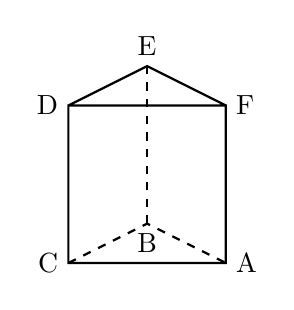
\begin{tikzpicture}
                    \draw[dashed,thick] (-1,0) node[left]{C} -- (0,0.5) node[below]{B} edge (0,2.5) -- (1,0) node[right]{A};
                    \draw[thick] (-1,0) rectangle (1,2) node[right]{F} -- (0,2.5) node[above]{E} -- (-1,2) node[left]{D};
                \end{tikzpicture}
            \end{center}
    
            移動開始からの経過時刻を$n$として,$n\to\infty$の極限において,頂点Aにいる蟻が頂点Dからスタートした確率を求めよ.必要ならば,次を使って良い:
            \begin{quote}
                \textbf{実対称行列に対するゲルシュゴリンの定理}
    
                $n$次実対称行列$M=(M_{ij})_{i,j\in[n]}$の$i$行目の対角要素$M_{ii}$以外の絶対値の和を$M_i$とする.
                \[M_i:=\sum_{k=1,k\ne i}^n\abs{M_{ik}},\quad D_i:=\Brace{z\in\R\mid\abs{z-M_{ii}}\le M_i}\]
                に対して,$M$の任意の固有値は$D_i\;(i=1,\cdots,n)$のいずれかの内に存在する.
            \end{quote}
        \end{enumerate}
    \end{problem}
\end{tcolorbox}
\begin{proof}[\textbf{\underline{[解答例]}}]\mbox{}
    \begin{enumerate}
        \item $n=1$のとき,成立は明らか.$n>1$のとき,
        \[M^{n-1}=\begin{pmatrix}I_d&O_d\\(I_d-R^{n-1})(I_d-R)^{-1}L&R^{n-1}\end{pmatrix}\]
        を認めると,
        \begin{align*}
            M^n&=M^{n-1}M=\begin{pmatrix}I_d&O_d\\(I_d-R^{n-1})(I_d-R)^{-1}L&R^{n-1}\end{pmatrix}\begin{pmatrix}I_d&O_d\\L&R\end{pmatrix}\\
            &=\begin{pmatrix}I_d&O_d\\(I_d-R^n)(I_d-R)^{-1}L&R^n\end{pmatrix}.
        \end{align*}
        ただし左下成分については,
        \[(I_d-R^{n-1})(I_d-R^{-1})^{-1}L+R^{n-1}L=\Paren{(I_d-R^{n-1})(I_d-R^{-1})^{-1}+(R^{n-1}-R^n)(I_d-R^{-1})^{-1}}L=(I_d-R^n)(I_d-R)^{-1}L\]
        と計算出来る.
        \item 与えられたMarkov過程は,初期分布を$\paren{0,0,0,\frac{1}{3},\frac{1}{3},\frac{1}{3}}$とし,遷移行列を
        \[A:=\mtrx{I_3}{O_3}{L}{R},\quad L:=\frac{1}{5}\diag(2,2,3),\quad R:=\frac{1}{5}\begin{pmatrix}2&0&1\\0&2&1\\1&1&0\end{pmatrix}.\]
        とするものである.$R$は対称行列であるから,Gershgorinの定理から,$M$の任意の固有値は$\paren{-\frac{2}{5},\frac{4}{5}}$に含まれる.
        特に,$\lim_{n\to\infty}R^n=O_3$である.
        (1)と併せると,
        \[\lim_{n\to\infty}A^n=\mtrx{I_3}{O_3}{(I_3-R)^{-1}L}{O_3},\quad (I_3-R)^{-1}L=\begin{pmatrix}\frac{4}{3}&\frac{2}{3}&3\\\frac{2}{3}&\frac{4}{3}&3\\2&2&9\end{pmatrix}.\]
        以上より,
        \[\frac{\frac{4}{3}}{\frac{4}{3}+\frac{2}{3}+2}=\frac{1}{3}.\]
    \end{enumerate}
\end{proof}

\section{2021年1月実施}

\begin{tcolorbox}[colframe=ForestGreen, colback=ForestGreen!10!white,breakable,colbacktitle=ForestGreen!40!white,coltitle=black,fonttitle=\bfseries\sffamily,
    title=概観]
    \begin{enumerate}[{第}1{問}]
        \item 行列計算,微分は良いが,(3)は一般可逆行列を題材にした骨のある線型代数の問題.
        \item 重積分の変数変換を用いた求積を題材とした簡単な計算問題.
        \item 単純なMarkov連鎖についてその不変分布を求めさせる問題.
        \item 指数分布を題材にして,その無記憶性と,関連する確率変数の分布同等性を証明させる小問集合である.
    \end{enumerate}
\end{tcolorbox}

\subsection{第一問}

\begin{tcolorbox}[colframe=ForestGreen, colback=ForestGreen!10!white,breakable,colbacktitle=ForestGreen!40!white,coltitle=black,fonttitle=\bfseries\sffamily,
    title=第1問]
    \begin{problem}\mbox{}\label{prob-21-1-1-Generalized-Inverse}
        \begin{enumerate}
            \item 行列$A$とベクトル$b$を次のように定めたとき,$\rank(b,Ab,A^2b)$を求めよ:
            \[A:=\begin{pmatrix}0&1&0\\0&-1&1\\0&0&-1\end{pmatrix},\quad b:=\begin{pmatrix}0\\1\\0\end{pmatrix}.\]
            \item 次の関数を$x$について微分せよ:
            \[f(x):=\frac{x^2}{\sqrt{1+x^2}+x}.\]
            \item $x\in\R^n$に関する等式制約\[Cx=d\in\R^m\quad(C\in M_{mn}(\R),m\le n,\rank C=m)\]の下で,$\norm{x}^2$を最小にする$x\in\R^n$を求めよ.なお,ノルムはEuclidノルム$\norm{x}^2=\sum_{i\in[n]}x_i^2$とする.
        \end{enumerate}
    \end{problem}
\end{tcolorbox}
\begin{proof}[\textbf{\underline{[解答例]}}]\mbox{}
    \begin{enumerate}
        \item $Ab,A^2b$を計算すると,
        \[Ab=\begin{pmatrix}
            1\\-1\\0
        \end{pmatrix},\quad A^2b=\begin{pmatrix}-1\\1\\0\end{pmatrix}.\]
        $A^2b=-Ab$と,$Ab,b$が線型独立であることに注意すると,$\rank(b,Ab,A^2b)=2$.
        \item 商の微分則より,
        \begin{align*}
            f'(x)&=\frac{2x(\sqrt{1+x^2}+x)-x^2\paren{\frac{x}{\sqrt{1+x^2}}+1}}{(\sqrt{1+x^2}+x)^2}\\
            &=\frac{x}{\sqrt{1+x^2}}\frac{2+2x^2+2x\sqrt{1+x^2}-x^2-x\sqrt{1+x^2}}{(\sqrt{1+x^2}+x)^2}\\
            &=\frac{x}{\sqrt{1+x^2}}\frac{x^2+x\sqrt{1+x^2}+2}{(\sqrt{1+x^2}+x)^2}=\frac{x}{\sqrt{1+x^2}}\frac{2\sqrt{1+x^2}-x}{\sqrt{1+x^2}+x}.
        \end{align*}
        \item 解空間は$\R^n$の$m$次元affine部分空間であり,任意の$Cx=d$の解$x_0\in\R^n$を用いて$\Brace{x\in\R^n\mid Cx=d}=x_0+\Ker C$と表せ,特に$x_0\perp\Ker C$を満たすときの$x_0$が求める$x\in\R^n$である.
        実際,任意の解$x\in\R^n$は$x_0+x_1\in x_0+\Ker C$と表せるから,Pythagorasの定理から$\norm{x}^2=\norm{x_0}^2+\norm{x_1}^2\ge\norm{x_0}^2$が成り立つ.
        $x_0\in(\Ker C)^\perp=\Im C^*$より,$\exists_{y_0\in\R^m}\;x_0=C^*y_0$.元の式に代入して$d=CC^*y_0$であるから,$CC^*\in\GL_m(\R)$に注意すると$y_0=(CC^*)^{-1}d$.よって,$x_0=C^*y_0=C^*(CC^*)^{-1}d$.
    \end{enumerate}
\end{proof}
\begin{remarks*}[一般化逆行列]
    (3)の答えに現れる$C^*(CC^*)^{-1}\in M_{nm}(\R)$とは,$C\in M_{mn}(\R)$の一般化逆行列(の一つ,特にMoore-Penrose型と言われるもの\ref{def-Moore-Penrose})である.
\end{remarks*}

\subsection{第二問}

\begin{tcolorbox}[colframe=ForestGreen, colback=ForestGreen!10!white,breakable,colbacktitle=ForestGreen!40!white,coltitle=black,fonttitle=\bfseries\sffamily,
    title=第2問]
    \begin{problem}
        次の重積分を考える:
    \[I:=\iint_De^{x+y}\sin^2(x-2y)dxdy,\quad D:=\Brace{(x,y)\in\R^2\mid\pi\le x-2y\le 3\pi,0\le x+y\le\pi}.\]
    \begin{enumerate}
        \item 次の変数変換のJacobianを求めよ:
        \[\begin{pmatrix}u\\v\end{pmatrix}=\begin{pmatrix}1&-2\\1&1\end{pmatrix}\begin{pmatrix}x\\y\end{pmatrix}.\]
        \item 上の変数変換によって対応する積分領域$D$を,$xy$平面上と$uv$平面上でそれぞれ図示せよ.
        \item 積分$I$を求めよ.
    \end{enumerate}
    \end{problem}
\end{tcolorbox}
\begin{proof}[\textbf{\underline{[解答例]}}]\mbox{}
    \begin{enumerate}
        \item 変数変換は
        \[\begin{cases}
            u=x-2y\\
            v=x+y
        \end{cases}\]
        と表せるから,Jacobi行列は
        \[\begin{pmatrix}\pp{u}{x}&\pp{u}{y}\\\pp{v}{x}&\pp{u}{y}\end{pmatrix}=\begin{pmatrix}1&-2\\1&1\end{pmatrix}.\]
        この行列の行列式は3である.
        \item 省略する.
        \item 次のように計算できる:
        \begin{align*}
            I&=\iint_De^{x+y}\sin^2(x-2y)dxdy\\
            &=3\int^\pi_0 e^vdv\int^{3\pi}_\pi\sin^2udu\\
            &=\frac{3}{2}(e^\pi-1)\Square{u-\frac{\sin2 u}{2}}^{3\pi}_\pi=3\pi(e^\pi-1).
        \end{align*}
    \end{enumerate}
\end{proof}

\subsection{第三問}

\begin{tcolorbox}[colframe=ForestGreen, colback=ForestGreen!10!white,breakable,colbacktitle=ForestGreen!40!white,coltitle=black,fonttitle=\bfseries\sffamily,
    title=第3問]
    \begin{problem}\label{prob-21-1-3-ProMtrx}
        次を満たす時間について一様なMarkov連鎖$X=(X_n):\Om\times\N\to[2]$
        \[P[X_{n+1}=i|X_{n}=i]=p,\quad p\in(0,1)\setminus\Brace{1/2},n\in\N,i\in[2],\]
        を考える.$X_n$の$[2]$上の確率分布を$\b{x}_n:=(x_n,1-x_n)^\top$で表す.
        \begin{enumerate}
            \item このMarkov連鎖の遷移行列$P\in M_2([0,1])$を求めよ.
            \item $\b{x}_\infty:=\lim_{n\to\infty}\b{x}_n\in[0,1]^2$を求めよ.
            \item $\forall_{n\in\N}\;\norm{\b{x}_n-\b{x}_\infty}^2\le\frac{1}{2}\abs{2p-1}^{2n}$を示せ.
        \end{enumerate}
    \end{problem}
\end{tcolorbox}
\begin{proof}[\textbf{\underline{[解答例]}}]\mbox{}
    \begin{enumerate}
        \item \[\begin{cases}
            x_{n+1}=px_n+(1-p)(1-x_n)\\
            1-x_{n+1}=(1-p)x_{n}+p(1-x_n)
        \end{cases}\]
        より,
        \[\x_{n+1}=\vctr{x_{n+1}}{1-x_{n+1}}=\mtrx{p}{1-p}{1-p}{p}\x.\]
        \item まず$P$の対角化$Q$を求める.すると,直交行列$U\in O_2([0,1])$を用いた表示$P=U^{-1}QU$を用いて,$P^n=U^{-1}Q^nU$と表せるため,
        $\b{x}_n=U^{-1}Q^nU\b{x}_0$によって$\b{x}_n$が計算できることが期待できる.
        その後,$n\to\infty$の極限を取ることで答えに至るであろう.
        \begin{enumerate}
            \item 固有方程式$\det(P-I\lambda)=0$を解いて固有値を求めると次のようになる.固有方程式は
            \[\begin{vmatrix}p-\lambda&1-p\\1-p&p-\lambda\end{vmatrix}=(p-\lambda)^2-(1-p)^2=(2p-1-\lambda)(1-\lambda)=0\]
            と表せるから,$\lambda=1,2p-1$が解である.
            \item 対応する固有ベクトルを求めると,
            \begin{enumerate}
                \item $P\begin{pmatrix}x\\y\end{pmatrix}=\begin{pmatrix}x\\y\end{pmatrix}$の解空間は$\R \begin{pmatrix}1\\1\end{pmatrix}$と表せる.
                \item $P\begin{pmatrix}x\\y\end{pmatrix}=(2p-1)\begin{pmatrix}x\\y\end{pmatrix}$の解空間は$\R \begin{pmatrix}-1\\1\end{pmatrix}$と表せる.
            \end{enumerate}
            \item 以上により,基底変換行列を$U:=\frac{1}{\sqrt{2}}\begin{pmatrix}1&-1\\1&1\end{pmatrix}$とおくことが考えられる.
            実際,$Q:=\diag(1,2p-1)=U^{-1}PU$が成り立っている:
            \begin{align*}
                U^{-1}PU&=\frac{1}{2}\begin{pmatrix}1&1\\-1&1\end{pmatrix}\begin{pmatrix}p&1-p\\1-p&p\end{pmatrix}\begin{pmatrix}1&-1\\1&1\end{pmatrix}\\
                &=\frac{1}{2}\begin{pmatrix}1&1\\1-2p&2p-1\end{pmatrix}\begin{pmatrix}1&-1\\1&1\end{pmatrix}\\
                &=\begin{pmatrix}1&0\\0&2p-1\end{pmatrix}.
            \end{align*}
            \item 故に,
            \[P^n=UQ^nU^{-1}=\frac{1}{2}\begin{pmatrix}1&-1\\1&1\end{pmatrix} \begin{pmatrix}1&0\\0&(2p-1)^n\end{pmatrix}\begin{pmatrix}1&1\\-1&1\end{pmatrix}=\frac{1}{2}\begin{pmatrix}1+(2p-1)^n&1-(2p-1)^n\\1-(2p-1)^n&1+(2p-1)^n\end{pmatrix},\]
            であるから,
            $-1<2p-1<1$より,
            \[\lim_{n\to\infty}P^n=\frac{1}{2}\begin{pmatrix}1&1\\1&1\end{pmatrix}=:P^\infty.\]
            行列積の連続性より,
            \[\b{x}_\infty=\lim_{n\to\infty}P^n\b{x}_0=P^\infty\b{x}_0=\frac{1}{2}\begin{pmatrix}1&1\\1&1\end{pmatrix}\begin{pmatrix}x_0\\1-x_0\end{pmatrix}=\begin{pmatrix}\frac{1}{2}\\\frac{1}{2}\end{pmatrix}.\]
        \end{enumerate}
        \item $x_n-x_\infty=(P^n-P^\infty)x_0$であるが,
        \[P^n-P^\infty=\mtrx{1}{1}{1}{-1}\paren{\mtrx{1}{0}{0}{(2p-1)^n}-\mtrx{1}{0}{0}{0}}\mtrx{-1}{-1}{-1}{1}\paren{-\frac{1}{2}}=\frac{1}{2}\mtrx{(2p-1)^n}{-(2p-1)^n}{-(2p-1)^n}{(2p-1)^n}.\]
        であるから,
        \[x_n-x_\infty=\frac{1}{2}\mtrx{(2p-1)^n}{-(2p-1)^n}{-(2p-1)^n}{(2p-1)^n}\vctr{x_0}{1-x_0}=\frac{(2p-1)^n}{2}\vctr{2x_0-1}{-2x_0+1}.\]
        よって,
        \begin{align*}
            \norm{x_n-x_\infty}^2&=\frac{\abs{2p-1}^{2n}}{4}2(2x_0-1)^2\\
            &=\frac{\abs{2p-1}^{2n}}{2}(2x_0-1)^2\le\frac{\abs{2p-1}^{2n}}{2}.
        \end{align*}
        最後の不等式評価は$x_0\in(0,1)$による.
    \end{enumerate}
\end{proof}
\begin{remark*}[(2)の注意点]
    $P$は対称で正な確率行列であるから,極限は必ず$\frac{1}{2}\mtrx{1}{1}{1}{1}$になる\ref{remark-limit-of-probability-matrix}.
    よって,初期分布$x_0$に依らずに,$x_\infty$が定まるのである.
\end{remark*}
\begin{remark*}[(3)での作用素ノルム利用の可能性について]
    (3)の不等式は,任意の確率ベクトル$\b{x}_n\ge0$についてのみ成り立つ不等式である.実際,一般のベクトル$\b{x}_n=(x_n,1-x_n)^\top\in[0,1]^2$について,行列の作用素ノルムを用いて
    \begin{align*}
        \norm{\b{x}_n-\b{x}_\infty}^2&\le\norm{P^n-P^\infty}^2\norm{\b{x}_0}^2\\
        &\le\Norm{\frac{1}{2}\begin{pmatrix}(2p-1)^n&-(2p-1)^n\\-(2p-1)^n&(2p-1)^n\end{pmatrix}}^2\\
        &=\frac{(2p-1)^{2n}}{4}\Norm{\begin{pmatrix}1&-1\\-1&1\end{pmatrix}}^2,&A:=\begin{pmatrix}1&-1\\-1&1\end{pmatrix}\text{とする}
    \end{align*}
    と評価出来るが,肝心の$A$の作用素ノルムは$\norm{A}^2=4$となってしまう.
    行列$A$の固有値は$0,2$で,$2$に属する固有空間は$\R \begin{pmatrix}1\\-1\end{pmatrix}$と表され,この元は確率ベクトルではない.
    すなわち,$A$の作用素ノルムを達成するベクトルは確率ベクトルではない.
    \[\sup\Brace{\norm{Ax}\in\R_+\mid x\in[0,1]^2\text{は確率ベクトル}}=\sqrt{2}\]
    を用いて,なんとか作用素ノルムで議論を完走する方法はありえる.
\end{remark*}

\subsection{第四問}

\begin{tcolorbox}[colframe=ForestGreen, colback=ForestGreen!10!white,breakable,colbacktitle=ForestGreen!40!white,coltitle=black,fonttitle=\bfseries\sffamily,
    title=第4問]
    \begin{problem}\mbox{}\label{prob-21-1-4-Exp}
        \begin{enumerate}
            \item 次の$g:\R\to\R$に関する微分方程式の一般解を求めよ:
            \[\dd{g(t)}{t}=a(1-g(t)),\quad a>0.\]
            \item $\R_+$上に台を持つ連続分布に従う確率変数$X$について,次を満たすならば,$X$は指数分布$\Exp(a)\;(a>0)$に従うことを示せ:
            \[\forall_{x,y\in\R}\quad P[X>x+y|X>x]=P[X>y].\]
            \item $X_1,X_2,X_3\sim\Exp(a)\;(a>0)$を独立同分布とする.このとき,次の$U,V$は分布同等であることを示せ:
            \[U:=X_1+\frac{1}{2}X_2+\frac{1}{3}X_3,\quad V:=\max\Brace{X_1,X_2,X_3}.\]
        \end{enumerate}
    \end{problem}
\end{tcolorbox}
\begin{proof}[\textbf{\underline{[解答例]}}]\mbox{}
    \begin{enumerate}
        \item \[\dd{(1-g(t))}{t}=-\dd{g}{t}(t)=-a(1-g(t)).\]
        であるから,$1-g(t)=Ce^{-a}\;(C\in\R)$.
        すなわち,$g(t)=1-Ce^{-a}\;(C\in\R)$.
        \item 分布関数を$F(x):=\int^x_0f(t)dt$と定めると,与えられた条件は
        \[\frac{1-F(x+y)}{1-F(x)}=1-F(y)\quad\Leftrightarrow\quad 1-F(x+y)=1-F(x)-F(y)+F(x)F(y)\]
        に同値.両辺の$y=0$での微分係数を考えると,
        \[F'(x)=f(x)=f(0)(1-F(x))\]
        が必要だから,(1)から
        \[\int^x_0f(t)dt=F(x)=1-Ae^{-f(0)x}.\]
        $F$は分布関数だから,$F(0)=0$より$A=1$が必要で,$F(x)=1-e^{-f(0)x}$であるが,$a:=f(0)$を母数とする指数分布の分布関数である.
        \item $U,V$の特性関数$\varphi,\psi$が等しいことを証明する.
        \begin{enumerate}
            \item $U$の特性関数は,Fubiniの定理から
            \begin{align*}
                \varphi(u)&=\int_{\R_+^3}e^{iu\paren{x_1+\frac{1}{2}x_2+\frac{1}{3}x_3}}f(x_1)f(x_2)f(x_3)dx_1dx_2dx_3\\
                &=a^3\int_{\R_+}e^{(iu-a)x_1}dx_1\int_{\R_+}e^{\paren{\frac{iu}{2}-a}x_2}dx_2\int_{\R_+}e^{\paren{\frac{iu}{3}-a}x_3}dx_3\\
                &=-a^3\frac{1}{iu-a}\frac{2}{iu-2a}\frac{3}{iu-3a}.
            \end{align*}
            と計算できる.
            \item $V$の特性関数は,
            $V$の分布関数$F_V$が
            \[F_V(x)=P[V\le x]=P[X_1\le x,X_2\le x,X_3\le x]=F(x)^3=(1-e^{-ax})^3\]
            であることより,
            $V$の確率密度関数$f_V$が,\[f_V(x)=\dd{F_V(x)}{x}=3f(x)F(x)^2=3f(x)\paren{\int_0^xf(t)dt}^2=3a(1-e^{-ax})^2e^{-ax}=3ae^{-ax}(1-2e^{-ax}+e^{-2ax})\]
            であることに注意すれば,
            \begin{align*}
                \psi(u)&=\int_{\R_+}e^{iux}f_V(x)dx\\
                &=3a\int_{\R_+}\paren{e^{(iu-a)x}-2e^{(iu-2a)x}+e^{(iu-3a)x}}dx\\
                &=3a\paren{-\frac{1}{iu-a}+\frac{2}{iu-2a}-\frac{1}{iu-3a}}\\
                &=3a\frac{-(-u^3-5aui+6a^2)+2(-u^2-4aui+3a^2)-(-u^2-3aui+2a^2)}{(iu-a)(iu-2a)(iu-3)}\\
                &=3a\frac{-2a^2}{(iu-a)(iu-2a)(iu-3)}.
            \end{align*}
        \end{enumerate}
    \end{enumerate}
\end{proof}
\begin{remarks*}[無記憶性による指数分布の特徴付け]
    (2)の条件を無記憶性といい,これを持つ連続分布は指数分布に限る.
    分布関数$F$に対して$S:=1-F$を生存関数という.
\end{remarks*}

\section{2020年1月実施}

\begin{tcolorbox}[colframe=ForestGreen, colback=ForestGreen!10!white,breakable,colbacktitle=ForestGreen!40!white,coltitle=black,fonttitle=\bfseries\sffamily,
    title=概観]
    \begin{enumerate}[{第}1{問}]
        \item 小問集合は珍しく,解析系の問題が全て確率論の問題となった.
        \item 簡単な定積分の計算問題.
        \item Schur補行列の逆行列を題材にした,ブロック行列の計算規則についての問題.
        \item 指数分布を題材として,分布関数を通じた変換と順序統計量とを題材にした密度関数の変換を問う難しい確率論の問題.
    \end{enumerate}
\end{tcolorbox}

\subsection{第一問}

\begin{tcolorbox}[colframe=ForestGreen, colback=ForestGreen!10!white,breakable,colbacktitle=ForestGreen!40!white,coltitle=black,fonttitle=\bfseries\sffamily,
    title=第1問]
    \begin{problem}\mbox{}
        \begin{enumerate}
            \item 次の行列の逆行列を求めよ:
            \[\begin{pmatrix}2&1&1\\-1&0&2\\1&1&2\end{pmatrix}.\]
            \item 確率変数列$\{X_n\}\subset L^2(\Om)$が$\lim_{n\to\infty}E[X_n^2]=0$を満たすならば$\forall_{\ep>0}\;P[\abs{X_n}>\ep]=0$が成り立つことを示せ.
            \item 確率変数列$\{X_n\}\subset L^2(\Om)$であって,$\forall_{\ep>0}\;P[\abs{X_n}>\ep]=0$であるが$\lim_{n\to\infty}E[X_n^2]\ne0$であるものの例を挙げよ.
        \end{enumerate}
    \end{problem}
\end{tcolorbox}
\begin{proof}[\textbf{\underline{[解答例]}}]\mbox{}
    \begin{enumerate}
        \item 略.
        \item 任意の$\ep>0$を取る.$\ep<\abs{X_n}$ならば$\ep^2<\abs{X_n}^2$であるから,事象集合について
        \[\Brace{\om\in\Om\mid\ep<\abs{X_n(\om)}}\subset\Brace{\om\in\Om\mid\ep^2<\abs{X_n^2(\om)}}\]
        が成り立つ.よって,
        \begin{align*}
            (0\le)P[\ep<\abs{X_n}]&\le P[\ep^2<\abs{X_n}^2]\le\frac{E[\abs{X_n}^2]}{\ep^2}\xrightarrow{n\to\infty}0.
        \end{align*}
        \item 確率空間$([0,1],\B([0,1]),m)$上の実確率変数$Y_n:[0,1]\to\R$を
        \[Y_n:=\sqrt{n}1_{[0,1/n]}\quad(n\in\N^+)\]
        と定める.すると,$\lim_{n\to\infty}\frac{1}{n}=0$より,$\forall_{\ep>0}\;\exists_{N>0}\;\forall_{n\ge N}\;\frac{1}{n}<\ep$.
        よって,$\forall_{n\ge N}\;P[\abs{Y_n}>\ep]=0$より当然$\lim_{n\to\infty}P[\abs{Y_n}>\ep]=0$.
        一方で,$\forall_{n\in\N^+}\;E[Y_n^2]=1$である.
    \end{enumerate}
\end{proof}

\subsection{第二問}

\begin{tcolorbox}[colframe=ForestGreen, colback=ForestGreen!10!white,breakable,colbacktitle=ForestGreen!40!white,coltitle=black,fonttitle=\bfseries\sffamily,
    title=第2問]
    \begin{problem}
        次の定積分を求めよ:
        \begin{enumerate}
            \item \[\int^1_0\frac{dx}{x^2-x+1}.\]
            \item \[\int^1_0\frac{dx}{x^3+1}.\]
        \end{enumerate}
    \end{problem}
\end{tcolorbox}
\begin{proof}[\textbf{\underline{[解答例]}}]\mbox{}
    \begin{enumerate}
        \item $x-\frac{1}{2}=\frac{\sqrt{3}}{2}\tan\theta$によって変数変換を行うと,次のように計算できる:
        \begin{align*}
            \int^1_0\frac{dx}{x^2-x+1}&=\int^1_0\frac{1}{\paren{x-\frac{1}{2}}^2+\frac{3}{4}}dx\\
            &=\int^{\pi/6}_{-\pi/6}\frac{4}{3}\frac{1}{\tan^2\theta+1}\frac{\sqrt{3}}{2}\frac{d\theta}{\cos^2\theta}\\
            &=\int^{\pi/6}_{-\pi/6}\frac{4}{3}\frac{\sqrt{3}}{2}d\theta
            =\int^{\pi/6}_{-\pi/6}\frac{2}{\sqrt{3}}=\frac{2\pi}{3\sqrt{3}}.
        \end{align*}
        \item 被積分関数の部分分数分解
        \[\frac{1}{x^3+1}=\frac{1}{3}\paren{\frac{1}{x+1}-\frac{x-2}{x^2-x+1}}\]
        を考えることにより,次のように計算できる.
        \begin{align*}
            \int^1_0\frac{dx}{x^3+1}&=\frac{1}{3}\int^1_0\paren{\frac{1}{x+1}-\frac{x-2}{x^2-x+1}}dx\\
            &=\frac{1}{3}\int^1_0\frac{dx}{x+1}-\frac{1}{6}\int^1_0\frac{(x^2-x+1)'}{x^2-x+1}dx+\frac{2}{3}\int^1_0\frac{dx}{x^2-x+1}\\
            &=\frac{\log 2}{3}+\frac{4}{9\sqrt{3}}\pi.
        \end{align*}
    \end{enumerate}
\end{proof}

\subsection{第三問}

\begin{tcolorbox}[colframe=ForestGreen, colback=ForestGreen!10!white,breakable,colbacktitle=ForestGreen!40!white,coltitle=black,fonttitle=\bfseries\sffamily,
    title=第3問]
    \begin{problem}\label{prob-20-1-3}
        この問題で登場する行列は全て$n\times n$の可逆行列であるとする.ブロック行列
        \[A=\begin{pmatrix}
            A_{11}&A_{12}\\A_{21}&A_{22}
        \end{pmatrix},\quad B=\begin{pmatrix}B_{11}&O\\B_{21}&B_{22}\end{pmatrix},\quad A_{11},A_{12},A_{21},A_{22},B_{11},B_{21},B_{22}\in\GL_n(\R).\]
        を考える.
        \begin{enumerate}
            \item 次を満たす行列$Q_1\in M_n(\R)$を$A_{11},A_{12},A_{21},A_{22}$とその逆行列を用いて表せ:
            \[\begin{pmatrix}
                A_{11}&A_{12}\\A_{21}&A_{22}
            \end{pmatrix}=\begin{pmatrix}A_{11}&O\\A_{21}&Q_1\end{pmatrix}\begin{pmatrix}I_n&Q_2\\O&I_n\end{pmatrix}.\]
            \item 次を満たす行列$Q_3\in M_n(\R)$を$B_{11},B_{21},B_{22}$とその逆行列を用いて表せ:
            \[\begin{pmatrix}
                B_{11}&O\\B_{21}&B_{22}
            \end{pmatrix}^{-1}=\begin{pmatrix}
                B_{11}^{-1}&O\\Q_3&B_{22}^{-1}
            \end{pmatrix}\]
            \item 次の行列の成分$A^{11},A^{12},A^{21},A^{22}$を$A_{11},A_{12},A_{21},A_{22}$とその逆行列を用いて表せ:
            \[A^{-1}=\begin{pmatrix}
                A^{11}&A^{12}\\A^{21}&A^{22}
            \end{pmatrix}\]
            \item 次の等式を示せ:
            \[(A_{22}-A_{21}A_{11}^{-1}A_{12})^{-1}=A_{22}^{-1}+A_{22}^{-1}A_{21}(A_{11}-A_{12}A_{22}^{-1}A_{21})^{-1}A_{12}A_{22}^{-1}.\]
        \end{enumerate}
    \end{problem}
\end{tcolorbox}
\begin{proof}[\textbf{\underline{[解答例]}}]\mbox{}
    \begin{enumerate}
        \item 右辺を計算すると
        \[\begin{pmatrix}
            A_{11}&A_{12}\\A_{21}&A_{22}
        \end{pmatrix}=\begin{pmatrix}A_{11}&O\\A_{21}&Q_1\end{pmatrix}\begin{pmatrix}I_n&Q_2\\O&I_n\end{pmatrix}=\begin{pmatrix}A_{11}&A_{11}Q_2\\A_{21}&A_{21}Q_2+Q_1\end{pmatrix}\]
        となるから,
        \[\begin{cases}
            A_{12}=A_{11}Q_2\\
            A_{22}=A_{21}Q_2+Q_1
        \end{cases}\quad\Leftrightarrow\quad 
        \begin{cases}
            Q_2=A_{11}^{-1}A_{12}\\
            Q_1=A_{22}-A_{21}A_{11}^{-1}A_{12}
        \end{cases}
        \]
        が必要.
        \item 
        \[\begin{pmatrix}I_n&O\\B_{21}B_{11}^{-1}+B_{22}Q_3&I_n\end{pmatrix}=\begin{pmatrix}
            B_{11}&O\\B_{21}&B_{22}
        \end{pmatrix}\begin{pmatrix}B_{11}^{-1}&O\\Q_3&B_{22}^{-1}\end{pmatrix}=I_{2n}\]
        が必要.
        よって,$Q_3=-B_{22}^{-1}B_{21}B_{11}^{-1}$.
        \item まず,$\begin{pmatrix}I_n&Q_2\\O&I_n\end{pmatrix}$の逆行列は$\begin{pmatrix}I_n&-Q_2\\O&I_n\end{pmatrix}$である.
        実際,
        \[\begin{pmatrix}I_n&Q_2\\O&I_n\end{pmatrix}\begin{pmatrix}I_n&-Q_2\\O&I_n\end{pmatrix}=I_{2n},\quad \begin{pmatrix}I_n&-Q_2\\O&I_n\end{pmatrix}\begin{pmatrix}I_n&Q_2\\O&I_n\end{pmatrix}=I_{2n}\]
        が成り立つ.よって,
        \begin{align*}
            \begin{pmatrix}
                A_{11}&A_{12}\\A_{21}&A_{22}
            \end{pmatrix}^{-1}&=\begin{pmatrix}I_n&Q_2\\O&I_n\end{pmatrix}^{-1}\begin{pmatrix}A_{11}&O\\A_{21}&Q_1\end{pmatrix}^{-1}\\
            &=\begin{pmatrix}I_n&-Q_2\\O&I_n\end{pmatrix}\begin{pmatrix}A_{11}^{-1}&O\\-Q_1^{-1}A_{21}A_{11}^{-1}&Q_1^{-1}\end{pmatrix}\\
            &=\begin{pmatrix}I_n&-A_{11}^{-1}A_{12}\\O&I_n\end{pmatrix}\begin{pmatrix}A_{11}^{-1}&O\\-(A_{22}-A_{21}A_{11}^{-1}A_{12})^{-1}A_{21}A_{11}^{-1}&(A_{22}-A_{21}A_{11}^{-1}A_{12})^{-1}\end{pmatrix}\\
            &=\begin{pmatrix}A_{11}^{-1}+A_{11}^{-1}A_{12}(A_{22}-A_{21}A_{11}^{-1}A_{12})^{-1}A_{21}A_{11}^{-1}&-A_{11}^{-1}A_{12}(A_{22}-A_{21}A_{11}^{-1}A_{12})^{-1}\\-(A_{22}-A_{21}A_{11}^{-1}A_{12})^{-1}A_{21}A_{11}^{-1}&(A_{22}-A_{21}A_{11}^{-1}A_{12})^{-1}\end{pmatrix}
        \end{align*}
        \item $A^{-1}$をもう一通りで表す.元の行列のUL分解を考えると,
        \[\mtrx{A_{11}}{A_{12}}{A_{21}}{A_{22}}=\mtrx{I}{R_2}{O}{I}\mtrx{R_1}{O}{A_{21}}{A_{22}}=\mtrx{R_1+R_2A_{21}}{R_2A_{22}}{A_{21}}{A_{22}}\]
        より,
        \[R_2=A_{12}A_{22}^{-1},\quad R_1=A_{11}-A_{12}A_{22}^{-1}A_{21}.\]
        続いて,このL部分の逆行列は
        \[\mtrx{R_1^{-1}}{O}{-A_{22}^{-1}A_{21}R_1^{-1}}{A_{22}^{-1}}\]
        と表せるから,
        \begin{align*}
            \mtrx{A_{11}}{A_{12}}{A_{21}}{A_{22}}^{-1}&=\paren{\mtrx{I}{R_2}{O}{I}\mtrx{R_1}{O}{A_{21}}{A_{22}}}^{-1}\\
            &=\mtrx{R_1^{-1}}{O}{-A_{22}^{-1}A_{21}R_1^{-1}}{A_{22}^{-1}}\mtrx{I}{-R_2}{O}{I}\\
            &=\mtrx{R_1^{-1}}{-R_1^{-1}R_2}{-A_{22}^{-1}A_{21}R_1^{-1}}{A_{22}^{-1}A_{21}R_1^{-1}R_2+A_{22}^{-1}}\\
            &=\mtrx{(A_{11}-A_{12}A_{22}^{-1}A_{21})^{-1}}{-(A_{11}-A_{12}A_{22}^{-1}A_{21})^{-1}A_{12}A_{22}^{-1}}{-A_{22}^{-1}A_{12}(A_{11}-A_{12}A_{22}^{-1}A_{21})^{-1}}{A_{22}^{-1}A_{21}(A_{11}-A_{12}A_{22}^{-1}A_{21})^{-1}A_{12}A_{22}^{-1}+A_{22}^{-1}}.
        \end{align*}
        以上より,$A^{-1}$の成分$A^{22}$を比べることで,
        \[(A_{22}-A_{21}A_{11}^{-1}A_{12})^{-1}=A_{22}^{-1}A_{21}(A_{11}-A_{12}A_{22}^{-1}A_{21})^{-1}A_{12}A_{22}^{-1}+A_{22}^{-1}\]
    \end{enumerate}
\end{proof}

\subsection{第四問}

\begin{tcolorbox}[colframe=ForestGreen, colback=ForestGreen!10!white,breakable,colbacktitle=ForestGreen!40!white,coltitle=black,fonttitle=\bfseries\sffamily,
    title=第4問]
    \begin{problem}\label{prob-20-1-4-Exp}
        $X_1,X_2,X_3$を独立同分布確率変数とし,その分布関数を$F$で表す.
        $F$は狭義単調増加かつ連続で,従って逆関数$F^{-1}$を持つとする.
        $E_1,E_2,E_3$を標準指数分布$\Exp(1)$に従う独立同分布確率変数とする.
        それぞれ3つの中で,昇順の並び替えを$X_{(1)}\le X_{(2)}\le X_{(3)},E_{(1)}\le E_{(2)}\le E_{(3)}$とする.
        \begin{enumerate}
            \item $(F^{-1}(e^{-E_{(1)}}),F^{-1}(e^{-E_{(2)}}),F^{-1}(e^{-E_{(3)}}))$と$(X_{(3)},X_{(2)},X_{(1)})$は同分布であることを示せ.
            \item $(E_{(1)},E_{(2)},E_{(3)})$の同時確率密度関数を求めよ.
            \item $3E_{(1)},2(E_{(2)}-E_{(1)}),E_{(3)}-E_{(2)}$は独立に標準指数分布に従うことを示せ.
            \item 次の確率変数の密度関数を求めよ:
            \[\log\log\paren{\frac{1}{F(X_{(2)})}}-\log\log\paren{\frac{1}{F(X_{(3)})}}\]
        \end{enumerate}
    \end{problem}
\end{tcolorbox}
\begin{proof}[\textbf{\underline{[解答例]}}]
    $\Exp(1)$の密度関数を$g(t)=e^{-t}1_{\R^+}$で表す.
    \begin{enumerate}
        \item 一般に,$E\sim\Exp(1)$のとき,$Y:=e^{-E}\sim\rU([0,1])$である.
        実際,この変換は$E\in\R^+$と$Y\in(0,1)$の間の可微分同相で,逆は$T(y)=-\log y$と表せ,
        $Y$の密度関数$p(y)$は,
        \begin{align*}
            p(y)&=g(T(y))\Abs{\dd{T}{y}}\\
            &=e^{-\log y}\frac{1}{y}=1.
        \end{align*}
        と計算できる.
        次に,$F^{-1}(Y)$の分布は,$e^{-E}\sim\rU((0,1))$より,
        \[P[F^{-1}(e^{-E})\le a]=P[e^{-E}\le F(a)]=F(a)\]
        であるから,$F^{-1}(e^{-E_1})$は$X_1$に分布が等しい.
        後は順序を考えると,$e^{-E_{(1)}}\ge e^{-E_{(2)}}\ge e^{-E_{(3)}}$で,$F^{-1}$も順序を保存するから,
        分布は$X_1,X_2,X_3$を降順に並び替えた確率ベクトル,すなわち$(X_{(3)},X_{(2)},X_{(1)})$に等しい.
        \item 次のように計算できる:
        \begin{align*}
            f(x,y,z)&=P[E_{(1)}=x,E_{(2)}=y,E_{(3)}=z]\\
            &=\begin{cases}
                6P[E_1=x,E_2=y,E_3=z]&x\le y\le z\text{のとき}\\
                0&\otherwise
            \end{cases}\\
            &=6e^{-(x+y+z)}1_{\Brace{x\le y\le z}}.
        \end{align*}
        \item 求める密度関数を$f$とすると,
        \begin{align*}
            f(y_1,y_2,y_3)&=P[3E_{(1)}=y_1,2(X_{(2)}-X_{(1)})=y_2,X_{(3)}-X_{(2)}=y_3]\\
            &=3!P[3E_1=y_1,2(X_2-X_1)=y_2,X_3-X_2=y_3]\\
            &=6\cdot\frac{1}{6}e^{-\frac{y_1}{3}}e^{-\frac{y_2}{2}-\frac{y_1}{3}}e^{-\frac{y_1}{3}-\frac{y_2}{2}-y_3}=e^{-y_1-y_2-y_3}.
        \end{align*}
        途中の計算は,変換
        \[\begin{cases}
            Y_1=3E_1\\
            Y_2=2(E_2-E_1)\\
            Y_3=E_3-E_2
        \end{cases}\Leftrightarrow\begin{cases}
            E_1=\frac{1}{3}Y_1\\
            E_2=\frac{Y_1}{3}+\frac{Y_2}{2}\\
            E_3=\frac{Y_1}{3}+\frac{Y_2}{2}+Y_3
        \end{cases}\]
        を考えると,$(E_1,E_2,E_3)\in(\R_+)^3$から$(Y_1,Y_2,Y_3)\in\R_+\times\R^2$上の可微分同相を定めており,
        Jacobianは$-\frac{1}{6}$で一定であるため.
        \item 問1から,$\paren{-\log F(X_{(3)}),-\log F(X_{(2)}),-\log F(X_{(1)})}$は$(E_{(1)},E_{(2)},E_{(3)})$に分布同等である.
        よって,
        \[Z_1:=\log\log\paren{\frac{1}{F(X_{(2)})}}-\log\log\paren{\frac{1}{F(X_{(3)})}}\]
        とおくと,
        \[e^{Z_1}=\frac{\log\frac{1}{F(X_{(2)})}}{\log\frac{1}{F(X_{(3)})}}=\frac{\log F(X_{(2)})}{\log F(X_{(3)})}\overset{d}{=}\frac{E_{(2)}}{E_{(1)}}.\]
        ここで,$(E_{(1)},E_{(2)})$の周辺密度関数は,結合密度関数$f(x,y,z)=6e^{-(x+y+z)}1_{\Brace{x\le y\le z}}$を$z$について積分することより,
        \begin{align*}
            f_{1,2}(x,y)&=\int^{z=\infty}_{z=y}6e^{-(x+y+z)}1_{\Brace{x\le y}}dz
            =\SQuare{-6e^{-(x+y+z)}1_{\Brace{x\le y}}}^{z=\infty}_{z=y}=6e^{-(x+2y)}1_{\Brace{x\le y}}.
        \end{align*}
        続いて,$Z_2:=E_{(1)}$と定めて,変換
        \[\begin{cases}
            Z_1=\log E_{(2)}-\log E_{(1)}\\
            Z_2=E_{(1)}
        \end{cases}\Leftrightarrow\begin{cases}
            E_{(1)}=Z_2\\
            E_{(2)}=Z_2e^{Z_1}
        \end{cases}\]
        を考えると,これは$(E_{(1)},E_{(2)})\in\Brace{(x,y)\in\R^2\mid0\le x\le y}$と$(\R_+)^2$との間の可微分同相を定めており,勾配行列とJacobianは
        \[\pp{(Z_1,Z_2)}{(E_{(1)},E_{(2)})}=\mtrx{0}{1}{Z_2e^{Z_1}}{e^{Z_1}},\qquad J(Z_1,Z_2)=-Z_2e^{Z_1}.\]
        以上より,$(Z_1,Z_2)$の結合密度関数$p$は,
        \begin{align*}
            p(z_1,z_2)&=6e^{-(z_2+2z_2e^{z_1})}\abs{z_2e^{z_1}}.
        \end{align*}
        よって,$Z_1$の周辺密度関数は,
        \begin{align*}
            p(z_1)&=\int^\infty_0p(z_1,z_2)dz_2\\
            &=\int^\infty_06e^{-(z_2+2z_2e^{z_1})}z_2e^{z_1}dz_2\\
            &=\SQuare{-\frac{6}{1+2e^{z_1}}e^{-(z_2+2z_2e^{z_1})}z_2e^{z_1}}^\infty_0+\int^\infty_0\frac{6}{1+2e^{z_1}}e^{-(z_2+2z_2e^{z_1})}e^{z_1}dz_2\\
            &=0+\SQuare{-\frac{6}{(1+2e^{z_1})^2}e^{-(z_2+2z_2e^{z_1})}e^{z_1}}^\infty_0=\frac{6}{(1+2e^{z_1})^2}e^{z_1}.
        \end{align*}
    \end{enumerate}
\end{proof}

\section{2019年8月実施}

\begin{tcolorbox}[colframe=ForestGreen, colback=ForestGreen!10!white,breakable,colbacktitle=ForestGreen!40!white,coltitle=black,fonttitle=\bfseries\sffamily,
    title=概観]
    \begin{enumerate}[{第}1{問}]
        \item Poisson分布の2,3次の積率を求める問題として,Taylor展開関連の計算問題だけ骨があった.
        \item 射影行列の階数や固有値に関連する性質を導出させる証明問題.
        \item 1階線型方程式の解放と数値近似を題材にした計算問題.
        \item 指数分布確率変数の商の密度と期待値を計算させる積分の計算問題.
    \end{enumerate}
\end{tcolorbox}

\subsection{第一問}

\begin{tcolorbox}[colframe=ForestGreen, colback=ForestGreen!10!white,breakable,colbacktitle=ForestGreen!40!white,coltitle=black,fonttitle=\bfseries\sffamily,
    title=第1問]
    \begin{problem}\mbox{}
        \begin{enumerate}
            \item 次の行列$M$の逆行列を求めよ:
            \[M=\begin{pmatrix}2&1&0\\1&0&1\\0&1&2\end{pmatrix}\]
            \item 次の定積分を求めよ:
            \[\int^1_{-1}\frac{x-1}{x^2+2x+5}dx.\]
            \item $\lambda\in\R$について,次の等式を示せ:
            \[\sum_{k\in\N}(k-\lambda)^2\frac{\lambda^ke^{-\lambda}}{k!}=\lambda,\quad\sum_{k\in\N}(k-\lambda)^3\frac{\lambda^ke^{-\lambda}}{k!}=\lambda.\]
            \item $d$-次元確率変数$X$について,$E[X]=\b{0}_d,\Var[X]=I_d$とする.このとき,正方行列$A\in M_d(\R)$が定める二次形式$X^\top AX$の期待値$E[X^\top AX]$を求めよ.
        \end{enumerate}
    \end{problem}
\end{tcolorbox}
\begin{proof}[\textbf{\underline{[解答例]}}]\mbox{}
    \begin{enumerate}
        \item $\frac{1}{4}\begin{pmatrix}1&2&-1\\2&-4&2\\-1&2&1\end{pmatrix}$.
        \item \begin{align*}
            \int^1_{-1}\frac{x-1}{x^2+2x+5}dx&=\int^1_{-1}\frac{x+1}{x^2+2x+5}dx-2\int^1_{-1}\frac{1}{x^2+2x+5}dx
        \end{align*}
        と分解して,第一項は$\frac{1}{2}\frac{(x^2+2x+5)'}{x^2+2x+5}$とみて,第二項は$x+1=2\tan\theta$の置換により,$\frac{\log 2}{2}-\frac{\pi}{4}$.
        \item それぞれの式をPoisson分布の2次と3次の中心積率を表していると見て,$\mu_2,\mu_3$とおく.
        Poisson分布の積率母関数は$M(t)=e^{\lambda(e^t-1)}$と表せるから,
        \[M'(t)=\lambda e^{t}M(t),\quad M''(t)=(\lambda^2 e^{2t}+\lambda e^t)e^{\lambda(e^t-1)}.\]
        \[M'''(t)=(\lambda^3e^{3t}+3\lambda^2e^{2t}+\lambda e^t)e^{\lambda(e^t-1)}.\]
        の$t=0$での値を考えることで,積率は$\al_1=\lambda,\al_2=\lambda^2+\lambda,\al_3=\lambda^3+3\lambda^2+\lambda$.
        よって,
        \[\mu_2=\al_2-2\lambda\al_1+\lambda^2=(\lambda^2+\lambda)-2\lambda\lambda+\lambda^2=\lambda.\]
        \[\mu_3=\al_3-3\lambda\al_2+3\lambda^2\al_1-\lambda^3=\lambda.\]
        \item $E[x^\top Ax]=\Tr(A)$.実際,
        \begin{align*}
            E[x^\top Ax]&=E\Square{x_1\sum_{j=1}^na_{1j}x_j+x_2\sum_{j=1}^na_{2j}x_j+\cdots+x_n\sum_{j=1}^na_{nj}x_j}\\
            &=a_{11}+a_{22}+\cdots+a_{nn}=\Tr(A).
        \end{align*}
    \end{enumerate}
\end{proof}

\subsection{第二問}

\begin{tcolorbox}[colframe=ForestGreen, colback=ForestGreen!10!white,breakable,colbacktitle=ForestGreen!40!white,coltitle=black,fonttitle=\bfseries\sffamily,
    title=第2問]
    \begin{problem}\label{prob-19-8-2}
        $d\ge3$とする.
    \begin{enumerate}
        \item 互いに直交する単位列ベクトル$a_1,a_2\in\R^d$に対して,行列$A\in M_d(\R)$を$A:=I_d-a_1a_1^\top-a_2a_2^\top$で定める.
        \begin{enumerate}
            \item $A^2=A$を示せ.
            \item $A$の固有値を求めよ.
        \end{enumerate}
        \item $B\in M_d(\R)$について,$\rank(B)+\rank(I_d-B)=d$ならば$B^2=B$であることを示せ.
    \end{enumerate}
    \end{problem}
\end{tcolorbox}
\begin{proof}[\textbf{\underline{[解答例]}}]\mbox{}
    \begin{enumerate}
        \item $a_1,a_2$は互いに直交する単位ベクトルであるから,
        \[(a_1a_1^\top)^2=a_1(a_1^\top a_1)a_1^\top =a_1a_1^\top,\quad (a_1a_1^\top)(a_2a_2^\top)=0\]
        で,$a_1,a_2$を逆にしても同様であることから,
        \begin{align*}
            A^2&=(I_d-a_1a_1^\top-a_2a_2^\top)(I_d-a_1a_1^\top-a_2a_2^\top)\\
            &=I_d+(a_1a_1^\top)^2+(a_2a_2^\top)^2-2a_1a_1^\top-2a_2a_2^\top+(a_1a_1^\top)(a_2a_2^\top)+(a_2a_2^\top)(a_1a_1^\top)\\
            &=I_d-a_1a_1^\top-a_2a_2^\top=A.
        \end{align*}
        $A$の固有値を$\lambda_1,\lambda_2,\cdots,\lambda_d\in\C$とし,$D:=\diag(\lambda_1,\cdots,\lambda_d)$とすると,$A=U^{-1}DU$を満たす正則行列$U\in\GL_d(\C)$が存在するから,$A^2=U^{-1}D^2U=U^{-1}DU=A$が必要.すなわち,$\lambda_i^2=\lambda_i\;(i=1,\cdots,d)$が必要.
        よって,$\lambda_1,\cdots,\lambda_d\in\{0,1\}$が必要.もし全て$0$であったら,
        $\rank A=0,\rank(a_1a_1^\top)=\rank(a_2a_2^\top)=1$より,
        $d\ge3$に矛盾.
        もし全て$1$であったら,
        \[Aa_1=(I_d-a_1a_1^\top-a_2a_2^\top)a_1=a_1-a_11-a_20=0\]
        より$\rank A<d$に矛盾.よって,$\Sp(A)=\{0,1\}$.
        \item $B(I_d-B)=O$を示せば良い.
        任意の$x\in\Im(B(I_d-B))$を取ると,$B(I_d-B)=(I_d-B)B$より
        $x\in\Im(B)\cap\Im(I_d-B)$であるが,次の議論より$\Im(B)\cap\Im(I_d-B)=0$である.

        一般に,\[\Ker(I_d-B)\subset\Im B,\quad\Ker(B)\subset\Im(I_d-B)\]である.$\rank B+\rank(I_d-B)=d$のとき,$\Ker B,\Ker(I_d-B)$の次元の和も$d$であるから,
        上式の包含関係$\subset$は実は$=$である.ここで,明らかに$\Ker(I_d-B)\cap\Ker(B)=0$であるから,$\Im(B)\cap\Im(I_d-B)=0$である.
    \end{enumerate}
\end{proof}

\subsection{第三問}

\begin{tcolorbox}[colframe=ForestGreen, colback=ForestGreen!10!white,breakable,colbacktitle=ForestGreen!40!white,coltitle=black,fonttitle=\bfseries\sffamily,
    title=第3問]
    \begin{problem}\mbox{}\label{prob-2019-8-3}
        \begin{enumerate}
            \item 微分方程式$\dd{x}{t}=f(t,x)$の解$x$について,
            \[\wh{x}(t_0+\Delta t):=x(t_0)+w_1\De tf(t_0,x_0)+w_2\De tf(t_0+\De t,x_0+\De x),\quad\De x=\De tf(t_0,x_0)\]
            が$x(t_0+\De t)$に対する2次近似になるように$w_1,w_2\in\R$を定めよ.
            \item 次の微分方程式の解で$x=\al t+\beta$の形を持つものを求めよ:
            \[\dd{x}{t}=-2(t+1)x-2t^2+1.\]
            \item (2)の微分方程式の一般解を求めよ.
            \item $t=0$のとき$x(0)=0$を満たす特殊解の$t=0.1$のときの$x$の値を(1)の近似を用いて小数第2位まで求めよ.
        \end{enumerate}
    \end{problem}
\end{tcolorbox}
\begin{proof}[\textbf{\underline{[解答例]}}]\mbox{}
    \begin{enumerate}
        \item $x$の$t_0$での3次についてのTaylor定理を考えると,
        \begin{align*}
            x(t_0+\De t)&=x(t_0)+\dd{x}{t}(t_0)\De t+\frac{1}{2}\dd{^2x}{t^2}(t_0)(\De t)^2+o(\abs{\De t}^3)\\
            &=x(t_0)+f(t_0,x_0)\De t+\frac{1}{2}\paren{\pp{f}{t}(t_0,x_0)+\pp{f}{x}(t_0,x_0)f(t_0,x_0)}(\De t)^2+o(\abs{\De t}^3)
        \end{align*}
        より,$w_1=1,w_2=1/2$.
        \item 解の形を$x=\al t+\beta\;(\al,\beta\in\R)$と予想すると,与えられた微分方程式の左辺と右辺は
        \begin{align*}
            \LHS&=\al\\
            \RHS&=-2(t+1)(\al t+\beta)-2t^2+1\\
            &=-2(1+\al)t^2-2(\al+\beta)t-2\beta+1.
        \end{align*}
        これらが任意の$t\in\R$について一致するためには,$\al=-1,\beta=1$が必要.
        よって,$x=-t+1$が与えられた形の解である.
        \item 与えられた微分方程式は1階非斉次の線形方程式であるから,一般解は斉次化
        \[\dd{x}{t}=-2(t+1)x\]
        の一般解と$x(t)=-t+1$との重ね合わせとなる.
        斉次化は変数分離型であり,一般解として$x(t)=Ce^{-t^2-2t}\;(C\in\R)$が見つかるから,元の式の一般解は
        \[Ce^{-t^2-2t}-t+1,\qquad(C\in\R).\]
        \item 問3の一般解に$x(0)=0$の条件を課すと,$C=-1$が必要.
        この特殊解$x(t):=-e^{-t^2-2t}-t+1$について,問1を適用することより,近似値$\wt{x}$は
        \begin{align*}
            \wh{x}(0+0.1)&=x(0)+(0.1)\times f(0,0)+\frac{1}{2}(0.1)\times f(0.1,(0.1\times f(0.0)))\\
            &=(0.1)\times 1+\frac{1}{2}\times 0.1\times\Paren{-2(1.1)\times0.1-0.02+1}\\
            &=0.1+0.1\times(-0.11-0.01+1)=0.189\approx0.19.
        \end{align*}
    \end{enumerate}
\end{proof}

\subsection{第四問}

\begin{tcolorbox}[colframe=ForestGreen, colback=ForestGreen!10!white,breakable,colbacktitle=ForestGreen!40!white,coltitle=black,fonttitle=\bfseries\sffamily,
    title=第4問]
    \begin{problem}\label{prob-19-8-4-Exp-density}
        $X,Y\sim\Exp(1)$を独立同分布とする.
    \begin{enumerate}
        \item $Z:=\sqrt{\frac{Y}{X}}$の確率密度関数を求めよ.
        \item $E[Z]$を求めよ.
    \end{enumerate}
    \end{problem}
\end{tcolorbox}
\begin{proof}[\textbf{\underline{[解答例]}}]\mbox{}
    \begin{enumerate}
        \item 次によって定まる可微分同相:$T^{-1}:(\R^+)^2\to(\R^+)^2$を考える:
        \[\begin{cases}
            Z_1:=\sqrt{Y/X}\\
            Z_2:=X
        \end{cases}\Leftrightarrow\begin{cases}
            X=Z_2\\
            Y=Z_1^2Z_2
        \end{cases}\]
        すると,勾配行列とJacobianは
        \[DT(z_1,z_2)=\mtrx{0}{1}{2z_1z_2}{z_1^2},\qquad J_T(z_1,z_2)=-2z_1z_2.\]
        より,たしかに$(\R^+)^2$上でJacobianは消えない.よって,$(Z_1,Z_2)$の結合密度関数は,
        \begin{align*}
            p(z_1,z_2)&=e^{-z_2}e^{-z_1^2z_2}z_1z_2=2z_1z_2e^{-z_2(1+z_1^2)}
        \end{align*}
        と表せる.求める$Z_1$の周辺密度関数は,
        \begin{align*}
            p(z_1)&=\int_0^\infty p(z_1,z_2)dz_2=2z_1\int^\infty_0e^{-z_2(1+z_1^2)}z_2dz_2\\
            &=2z_1\SQuare{-\frac{e^{-z_2(1+z_1^2)}}{1+z_1^2}z_2}^\infty_0+2z_1\int^\infty_0\frac{e^{-z_2(1+z_1^2)}}{1+z_1^2}dz_2\\
            &=2z_1\SQuare{-\frac{e^{-z_2(1+z_1^2)}}{(1+z_1^2)^2}}^\infty_0=\frac{2z_1}{(1+z_1^2)^2}.
        \end{align*}
        \item $z_1=:\tan\theta$の変数変換により,次のように計算出来る:
        \begin{align*}
            E[Z_1]&=2\int^\infty_0\frac{z_1^2}{(1+z_1^2)^2}dz_1\\
            &=2\int^{\pi/2}_0\cos^2\theta d\theta=
            \int^{\pi/2}_0(1+\cos 2\theta)d\theta\\
            &=\SQuare{\theta+\frac{\sin2\theta}{2}}^{\pi/2}_0=\frac{\pi}{2}.
        \end{align*}
    \end{enumerate}
\end{proof}

\section{2019年1月実施}

\begin{tcolorbox}[colframe=ForestGreen, colback=ForestGreen!10!white,breakable,colbacktitle=ForestGreen!40!white,coltitle=black,fonttitle=\bfseries\sffamily,
    title=概観]
    \begin{enumerate}[{第}1{問}]
        \item 2018年8月実施分同様,明示的にMaclaurin展開の問題が出た.
        \item 中心化行列を題材とした固有値問題.
        \item 2つの小問からなり,積分計算問題と,Maclaurin展開を通じて極限を求める問題.
        \item 正規分布を題材に,その線型変換と商の密度を導出させる問題.
    \end{enumerate}
\end{tcolorbox}

\subsection{第一問}

\begin{tcolorbox}[colframe=ForestGreen, colback=ForestGreen!10!white,breakable,colbacktitle=ForestGreen!40!white,coltitle=black,fonttitle=\bfseries\sffamily,
    title=第1問]
    \begin{problem}\mbox{}
        \begin{enumerate}
            \item 次の行列$A\in M_2(\R)$に対して,$A^5$を求めよ:
            \[A=\mtrx{1}{-2}{-2}{4}.\]
            \item 次の関数を2次までMaclaurin展開せよ:$f(x)=\log(3+4x)$.
            \item 次の定積分の値を求めよ:
            \[\int^1_0\frac{1-x}{\sqrt{3+2x-x^2}}dx,\quad\int^1_0\frac{1}{\sqrt{3+2x-x^2}}dx.\]
            \item $V$を線型空間,$v_1,v_2,v_3\in V$を基底とする.
            新たな基底を
            \[u_1=v_1+v_2,\quad u_2=v_1-v_2+v_3,\quad u_3=-v_1+v_2+v_3\]
            と定めたとき,次のベクトル$a\in V$の$u_1,u_2,u_3$による成分表示を求めよ:
            \[a:=2v_1+4v_2+3v_3\in V\]
        \end{enumerate}
    \end{problem}
\end{tcolorbox}
\begin{proof}[\textbf{\underline{[解答例]}}]\mbox{}
    \begin{enumerate}
        \item 明らかに固有ベクトルからなる基底$(1,-2)^\top,(2,1)^\top$を持つから,
        \[\frac{1}{5}\mtrx{1}{-2}{2}{1}A\mtrx{1}{2}{-2}{1}=\mtrx{5}{0}{0}{0}\]
        と対角化できる.よって,
        \[A^5=\frac{1}{5}\mtrx{1}{2}{-2}{1}\mtrx{3125}{0}{0}{0}\mtrx{1}{-2}{2}{1}=625\mtrx{1}{-2}{-2}{4}=625A.\]
        \item $f$の2階までの導関数の$x=0$での値を求めることにより,
        \[\log(3+4x)=\log 3+\frac{4}{3}x-\frac{8}{9}x^2+O(x^3)\quad(\abs{x}\to0).\]
        \item \[\int^1_0\frac{1-x}{\sqrt{3+2x-x^2}}dx=\Square{\sqrt{3+2x-x^2}}^1_0=2-\sqrt{3}.\]
        $x=1+2\sin\theta$と置換することにより,
        \begin{align*}
            \int^1_0\frac{1}{\sqrt{3+2x-x^2}}dx&=\int^0_{-\frac{\pi}{6}}\frac{1}{2\cos\theta}2\cos\theta d\theta=\frac{\pi}{6}.
        \end{align*}
        \item 基底変換行列を
        \[(u_1\;u_2\;u_3)=(v_1\;v_2\;v_3)\underbrace{\begin{pmatrix}
            1&1&-1\\1&-1&1\\0&1&1
        \end{pmatrix}}_{=:P}\]
        と定めると,
        \[a=(v_1\;v_2\;v_3)\begin{pmatrix}
            2\\4\\3
        \end{pmatrix}=(u_1\;u_2\;u_3)P^{-1}\begin{pmatrix}
            2\\4\\3
        \end{pmatrix}=(u_1\;u_2\;u_3)\begin{pmatrix}
            2&2&0\\1&-1&2\\-1&1&2
        \end{pmatrix}\begin{pmatrix}
            2\\4\\3
        \end{pmatrix}=(u_1\;u_2\;u_3)\begin{pmatrix}
            12\\4\\8
        \end{pmatrix}.\]
    \end{enumerate}
\end{proof}

\subsection{第二問}

\begin{tcolorbox}[colframe=ForestGreen, colback=ForestGreen!10!white,breakable,colbacktitle=ForestGreen!40!white,coltitle=black,fonttitle=\bfseries\sffamily,
    title=第2問]
    \begin{problem}\label{prob-19-1-2}
        $N\in\N,a\in\R$について,
        \[A_N:=\begin{pmatrix}
            1-a&-a&\cdots&-a\\
            -a&1-a&\ddots&\vdots\\
            \vdots&\ddots&\ddots&-a\\
            -a&\cdots&-a&1-a
        \end{pmatrix}\in M_N(\R)\]
        と定める.
        また,
        \[T_5=\begin{pmatrix}
            1&0&0&0&0\\
            -1&1&0&0&0\\
            -1&0&1&0&0\\
            -1&0&0&1&0\\
            -1&0&0&0&1
        \end{pmatrix}\]
        と定める.
        \begin{enumerate}
            \item $T_5A_5$を求めよ.
            \item $\det(A_5)$を求めよ.また,一般の$\det(A_N)$を求めよ.
            \item $0\in\Sp(A)$とする.このときの$a\in\R$と,固有値$0$に属する単位固有ベクトル$z$を求めよ.
            \item $0\in\Sp(A)$とする.$x:=A_N(I_N+A_N^2)^{-1}z$を求めよ.
        \end{enumerate}
    \end{problem}
\end{tcolorbox}
\begin{proof}[\textbf{\underline{[解答例]}}]\mbox{}
    \begin{enumerate}
        \item \[T_5A_5=\begin{pmatrix}
            1-a&-a&-a&-a&-a\\
            -1&1&0&0&0\\
            -1&0&1&0&0\\
            -1&0&0&1&0\\
            -1&0&0&0&1
        \end{pmatrix}.\]
        \item 行列式は,列ベクトルに関する多重交代線型形式であることに注意すると,第一列の分解$e_1+(-a,\cdots,-a)^\top$について,$\det(A_N)=\det(A_{N-1})+\det(B_N)$となる,ただし,$B_N$は行列$A_{N}$の第一列を$(-a,\cdots,-a)^{\top}$に変えたものとした.
        ここで同様の手続きを$B_N$の第二列に施すと,これは$B_{N-1}$と同じ行列式を持つことが判る.これを繰り返して,
        \[\det(A_N)=\det(A_{N-1})+\det(B_2)=\det(A_{N-1})-a.\]
        $\abs{A_1}=1-a,\abs{A_2}=1-2a$と繰り返し計算して,$\abs{A_5}=1-5a$.
        一般には$\abs{A_N}=1-Na$.
        \item $0\in\Sp(A_N)$のとき$\det(A_N)=0$より,$a=\frac{1}{N}$.
        このとき,$A_N$は
        \[A_N=I_N-\frac{1}{n}\begin{pmatrix}
            1&\cdots&1\\
            \vdots&\ddots&\vdots\\
            1&\cdots&1
        \end{pmatrix}\]
        という形の射影行列になるから,$0$に属する単位固有ベクトルの1つは
        \[z:=\frac{1}{\sqrt{N}}\begin{pmatrix}
            1\\\vdots\\1
        \end{pmatrix}\]
        と見つかる.
        \item 射影行列$A_N$は半正定値であるから,$I_N+A_N^2=I_N+A_N$はたしかに可逆である.
        また,$P_N:=I_N-A_N$とおくと,これも射影行列で,
        \[(I_N+P_N)(I_N+A_N)=(I_N+A_N)(I_N+P_N)=2I_N\]
        であるから,$(I_N+A_N)^{-1}=\frac{1}{2}(I_N+P_N)$とわかる.
        以上より,
        \[x=A_N\frac{1}{2}(I_N+P_N)z=A_Nz=0.\]
    \end{enumerate}
\end{proof}
\begin{remarks*}
    問題の$A_N$の形をした行列のことを\textbf{中心化行列}と言う.
    中心化行列はHouseholder行列の例であり,原点を通る超平面に関する鏡映変換を表す行列である.
    行列のQR分解の数値計算に使われる,
\end{remarks*}

\subsection{第三問}

\begin{tcolorbox}[colframe=ForestGreen, colback=ForestGreen!10!white,breakable,colbacktitle=ForestGreen!40!white,coltitle=black,fonttitle=\bfseries\sffamily,
    title=第3問]
    \begin{problem}\mbox{}
        \begin{enumerate}[{問}1]
            \item 関数
            \[f(x)=\frac{1}{1+(\tan x)^{\sqrt{2}}},\quad x\in\paren{0,\frac{\pi}{2}}\]
            について,
            \begin{enumerate}
                \item $\forall_{x\in(0,\pi/2)}\;f(x)+f\paren{\frac{\pi}{2}-x}=\const$を示せ.
                \item $f(x)$の$(0,\pi/2)$上での定積分の値を求めよ.
            \end{enumerate}
            \item 
            \begin{enumerate}
                \item $\log(1+x)$のMaclaurin展開を考えることより,$\frac{\log(1+x)}{x}$の2次近似式を求めよ.
                \item 次の極限が存在するための$a,b\in\R$の値と,そのときの極限値を求めよ:
                \[\lim_{x\to0}\frac{(1+x)^{\frac{1}{x}}-e(a+bx)}{x^2}.\]
            \end{enumerate}
        \end{enumerate}
    \end{problem}
\end{tcolorbox}
\begin{proof}[\textbf{\underline{[解答例]}}]\mbox{}
    \begin{enumerate}[{問}1]
        \item 任意の$x\in(0,\pi/2)$について,$\tan\paren{\frac{\pi}{2}-x}=\frac{1}{\tan x}$より,
        \[f(x)+f\paren{\frac{\pi}{2}-x}=\frac{1}{1+(\tan x)^{\sqrt{2}}}+\frac{1}{1+(\tan x)^{-\sqrt{2}}}=\frac{1+(\tan x)^{\sqrt{2}}}{1+(\tan x)^{\sqrt{2}}}=1.\]
        これを用いて,定積分の値を$I$とすると,
        \begin{align*}
            \frac{\pi}{2}&=\int^{\pi/2}_0\paren{f(x)+f\paren{\frac{\pi}{2}-x}}dx\\
            &=I+\int^{\pi/2}_0f\paren{\frac{\pi}{2}-x}dx\\
            &=I-\int^0_{\pi/2}f(y)dy=2I.
        \end{align*}
        以上より,
        \[I=\frac{\pi}{4}.\]
        \item \begin{enumerate}
            \item $\log(1+x)$の3階までの$x=0$での微分係数を計算することにより,
            \[\log(1+x)=x-\frac{x^2}{2}+\frac{x^3}{3}+O(x^4)\quad(\abs{x}\to0)\]
            を得る.よって,$\abs{x}<1$の範囲で,
            \[\frac{\log(1+x)}{x}=1-\frac{x}{2}+\frac{x^2}{3}+O(x^3)\quad(\abs{x}\to0).\]
            \item $(1+x)^{\frac{1}{x}}=e^{\frac{1}{x}\log(1+x)}$のMaclaurin展開を考えると,
            \begin{align*}
                (1+x)^{\frac{1}{x}}&=1+\paren{1-\frac{x}{2}+\frac{x^2}{3}+O(x^3)}+\frac{1}{2}\paren{1-\frac{x}{2}+\frac{x^2}{3}+O(x^3)}+\frac{1}{3!}\paren{1-\frac{x}{2}+\frac{x^2}{3}+O(x^3)}^2+\cdots\\
                &=\paren{1+1+\frac{1}{2}+\frac{1}{3!}+\cdots}-\frac{x}{2}\paren{1+1+\frac{1}{2}+\cdots}+\frac{x^2}{3}\paren{1+1+\frac{1}{2}+\cdots}+O(x^3)\\
                &=e\paren{1-\frac{x}{2}+\frac{x^2}{3}}+O(x^3)\qquad(\abs{x}\to0)
            \end{align*}
            を得る.よって,$a=1,b=-\frac{1}{2}$とおけば,極限値$\frac{1}{3}e$を得る.
        \end{enumerate}
    \end{enumerate}
\end{proof}

\subsection{第四問}

\begin{tcolorbox}[colframe=ForestGreen, colback=ForestGreen!10!white,breakable,colbacktitle=ForestGreen!40!white,coltitle=black,fonttitle=\bfseries\sffamily,
    title=第4問]
    \begin{problem}\label{prob-19-1-4}
        $X_1,X_2\sim N(0,1)$を独立同分布,
        \[\vctr{Y_1}{Y_2}=\mtrx{1}{a}{a}{1}\vctr{X_1}{X_2},\quad a\in(0,1).\]
        と定める.この問題では,正規分布に関する性質は,次の公式を除いて証明なしで用いてはならない:
        \[\int_\R e^{-\frac{x^2}{2}}dx=\sqrt{2\pi}.\]
        \begin{enumerate}
            \item 次を計算せよ:$E[X_1],\Var[X_1]$.
            \item $\Cov[Y_1,Y_2]$を計算せよ.
            \item $(Y_1,Y_2)$の同時確率密度関数が次で与えられることを示せ:
            \[f(y_1,y_2)=\frac{1}{2\pi(1-a^2)}\exp\paren{-\frac{1}{2(1-a^2)^2}\Paren{(1+a^2)y_1^2-4ay_1y_2+(1+a^2)y^2_2}}\quad(y_1,y_2)\in\R^2.\]
            \item 確率変数$\frac{Y_1}{Y_2}$の確率密度関数を求めよ.
        \end{enumerate}
    \end{problem}
\end{tcolorbox}
\begin{proof}[\textbf{\underline{[解答例]}}]\mbox{}
    \begin{enumerate}
        \item 次のように計算できる:
        \[E[X_1]=\frac{1}{\sqrt{2\pi}}\int_\R xe^{-\frac{x^2}{2}}dx=-\frac{1}{\sqrt{2\pi}}\int_\R\paren{-\frac{x^2}{2}}'e^{-\frac{x^2}{2}}dx=-\frac{1}{\sqrt{2\pi}}\SQuare{e^{-\frac{x^2}{2}}}^\infty_{-\infty}=0.\]
        \[\Var[X_1]=E[X_1^2]=-\frac{1}{\sqrt{2\pi}}\int_\R x\paren{-\frac{x^2}{2}}'e^{-\frac{x^2}{2}}dx=-0+\frac{1}{\sqrt{2\pi}}\int_\R e^{-\frac{x^2}{2}}dx=1.\]
        \item まず,$X_1\indep X_2$より$\Cov[X_1,X_2]=0$である.実際,Fubiniの定理より,
        \[\Cov[X_1,X_2]=E[X_1X_2]=\iint_{\R^2}x_1x_2e^{-\frac{x_1^2}{2}-\frac{x_2^2}{2}}dx_1dx_2=\int_{\R}x_1e^{-\frac{x_1^2}{2}}dx_1\int_\R x_2e^{-\frac{x_2^2}{2}}dx_2=0.\]
        よって,共分散の双線型性より,
        \[\Cov[Y_1,Y_2]=\Cov[X_1+aX_2,aX_1+X_2]=a\Var[X_1]+a\Var[X_2]=2a.\]
        なお,$\Var[Y_1]=\Var[Y_2]=a^2+1$である.
        \item \[\begin{cases}
            Y_1=X_1+aX_2=y_1\\
            Y_2=aX_1+X_2=y_2
        \end{cases}\quad\Leftrightarrow\quad\begin{cases}
            X_1=\frac{y_1-ay_2}{1-a^2}\\
            X_2=\frac{y_2-ay_1}{1-a^2}
        \end{cases}\]
        より,$N(0,1)$の確率密度関数を$\phi$で表すと,変換$(y_1,y_2)\mapsto(X_1,X_2)$のJacobianは$\frac{1}{1-a^2}$であるから,
        \begin{align*}
            f(y_1,y_2)&=\frac{1}{1-a^2}\phi\paren{\frac{y_1-ay_2}{1-a^2}}\phi\paren{\frac{y_2-ay_1}{1-a^2}}\\
            &=\frac{1}{1-a^2}\frac{1}{\sqrt{2\pi}}\exp\paren{-\paren{\frac{y_1-ay_2}{1-a^2}}^2\frac{1}{2}}\frac{1}{\sqrt{2\pi}}\exp\paren{-\paren{\frac{y_2-ay_1}{1-a^2}}^2\frac{1}{2}}\\
            &=\frac{1}{2\pi(1-a^2)}\exp\paren{-\frac{1}{2(1-a^2)^2}\Paren{(1+a^2)y_1^2-4ay_1y_2+(1+a^2)y_2^2}}.
        \end{align*}
        \item ここで,変数変換$T^{-1}(Y_1,Y_2)=(y,y_2)$を
        \[\begin{cases}
            \frac{Y_1}{Y_2}=y\\
            Y_2=y_2
        \end{cases}\quad\Leftrightarrow\quad\begin{cases}
            Y_1=yY_2=yy_2\\
            Y_2=y_2
        \end{cases}\]
        と定めると,$T:\R\times\R\setminus\{0\}\to\R\times\R\setminus\{0\}$は可微分同相であり,
        Jacobianは$y_2$であるから$\R\times\R\setminus\{0\}$上で消えない.
        よって,
        $(y,y_2)=\paren{\frac{Y_1}{Y_2},Y_2}$の結合分布密度関数は
        \[f(y,y_2)=\frac{\abs{y_2}}{2\pi(1-a^2)}\exp\paren{-\frac{y^2_2}{2(1-a^2)^2}\Paren{(1+a^2)y^2-4ay+(1+a^2)}}.\]
        これを$y_2$について積分することで,
        \begin{align*}
            f(y)&=\frac{1}{2\pi(1-a^2)}2\int^\infty_0y_2\exp\paren{-\frac{y^2_2}{2(1-a^2)^2}\Paren{(1+a^2)y^2-4ay+(1+a^2)}}dy_2\\
            &=\frac{1}{\pi(1-a^2)}\Square{-\frac{(1-a^2)^2}{\Paren{(1+a^2)y^2-4ay+(1+a^2)}}\exp\paren{-\frac{y^2_2}{2(1-a^2)^2}\Paren{(1+a^2)y^2-4ay+(1+a^2)}}}^\infty_0\\
            &=\frac{1}{\pi(1-a^2)}\frac{(1-a^2)^2}{\Paren{(1+a^2)^2y^2-4ay+(1+a^2)}}=\frac{1-a^2}{\pi\Paren{(1+a^2)y^2-4ay+(1+a^2)}}\\
            &=\frac{1}{\pi\frac{1-a^2}{1+a^2}}\frac{1}{1+\paren{\frac{y-\frac{2a}{1+a^2}}{\frac{1-a^2}{1+a^2}}}^2}.
        \end{align*}
    \end{enumerate}
\end{proof}
\begin{remark*}\mbox{}
    \begin{itemize}
        \item 問3の答えは,
        \[\Sigma:=\Cov[Y]=\mtrx{1+a^2}{2a}{2a}{1+a^2}\]
        について,
        \[\frac{1}{2\pi\sqrt{\det\Sigma}}\exp\paren{-\frac{1}{2}y^\top\Sigma^{-1}y},\qquad y:=(y_1,y_2)\in\R^2\]
        と表せているから,$\rN_2(0,\Sigma)$の密度関数である.
        \item 一般に,任意の正定値対称行列$\Sigma\in M_2(\R)$について,$(Y_1,Y_2)\sim\rN(0,\Sigma)$であるとき,
        \[\frac{Y_1}{Y_2}\sim\Cauchy\paren{\frac{\sigma_{12}}{\sigma_{22}},\frac{\sqrt{\det\Sigma}}{\sigma_{22}}}\]
        が成り立つ.
    \end{itemize}
\end{remark*}

\section{2018年8月実施}

\begin{tcolorbox}[colframe=ForestGreen, colback=ForestGreen!10!white,breakable,colbacktitle=ForestGreen!40!white,coltitle=black,fonttitle=\bfseries\sffamily,
    title=概観]
    \begin{enumerate}[{第}1{問}]
        \item とにかく計算量の多い微分と行列演算の小問であった.
        \item Gram行列を題材とした対称行列の対角化・固有値の標準的な問題.
        \item $\chi^2$-分布とその和・商の確率密度関数を特性関数を通じて導出する問題.
        \item 問1だけ特異的に難しい最適化問題(和で表される関数の最小化)を題材にした極値問題である.
    \end{enumerate}
    微分係数の計算が困難なMaclaurin展開,独立な$\chi^2$-確率変数の和や商の密度関数を復習すると良いだろう.
\end{tcolorbox}

\subsection{第一問}

\begin{tcolorbox}[colframe=ForestGreen, colback=ForestGreen!10!white,breakable,colbacktitle=ForestGreen!40!white,coltitle=black,fonttitle=\bfseries\sffamily,
    title=第1問]
    \begin{problem}\mbox{}
        \begin{enumerate}[{問}1]
            \item 次の行列が可逆か判定し,可逆ならば逆行列を,非可逆ならば右零因子を1つ求めよ.
            \[A:=\mtrx{1}{3}{2}{4},\qquad B:=\mtrx{1}{3}{3}{9}\]
            \item 次の関数の導関数を求めよ:
            \[f(x):=5^{x^2-3x+1},\qquad g(x):=\log\sqrt{\frac{1-x}{1+x}},\quad(\abs{x}<1).\]
            \item $f(x):=(1+x)^{\frac{1}{x}}$の2次までのMaclaurin展開を求めよ.
            \item 次の3つのベクトルが生成する$\R^4$の線型部分空間の正規直交基底を1組求めよ.
            \[a:=\begin{pmatrix}
                1\\2\\0\\1
            \end{pmatrix},\quad b:=\begin{pmatrix}
                2\\1\\0\\1
            \end{pmatrix},\quad c:=\begin{pmatrix}
                1\\0\\1\\2
            \end{pmatrix}\]
        \end{enumerate}
    \end{problem}
\end{tcolorbox}
\begin{proof}[\textbf{\underline{[解答例]}}]\mbox{}
    \begin{enumerate}
        \item $\det A=-2$より可逆で,逆行列は$\frac{1}{-2}\mtrx{4}{-3}{-2}{1}$.$\det B=0$より特異で,$\mtrx{-3}{-3}{1}{1}$は右の零因子である.
        \item $g'$の計算は,$\abs{x}<1$のとき$1-x,1+x>0$に注意して,
        \begin{align*}
            f'(x)&=(e^{\log 5(x^2-3x+1)})'=\log 5(2x-3)5^{x^2-3x+1}.\\
            g'(x)&=\paren{\frac{1}{2}\paren{\log(1-x)-\log(1+x)}}'=-\frac{1}{2}\frac{1}{1-x}-\frac{1}{2}\frac{1}{1+x}.
        \end{align*}
        \item $f(0)=\lim_{x\to 0}(1+x)^{\frac{1}{x}}=e$.両辺の対数を取って微分すると,
        \[\frac{f'(x)}{f(x)}=-\frac{\log(1+x)}{x^2}+\frac{1}{x(1+x)}=\frac{-(1+x)\log(1+x)+x}{x^2(1+x)}.\]
        右辺の$x=0$における極限はl'Hospitalの定理を繰り返し適用することより計算出来て,$f'(0)=f(0)\paren{-\frac{1}{2}}=-\frac{e}{2}$を得る.
        二次の微分係数も同様にして,
        \[f(x)=e-\frac{e}{2}x+\frac{11e}{24}x^2+O(x^3)\qquad(\abs{x}<1).\]
        \item \[e_1:=\frac{1}{\norm{a}}=\frac{1}{\sqrt{6}}
        \begin{pmatrix}
            1\\2\\0\\1
        \end{pmatrix}.\]
        次に,$b$の$e_1$の直交成分は
        \[b-\frac{a\cdot b}{\norm{a}^2}a=\begin{pmatrix}
            2\\1\\0\\1
        \end{pmatrix}-\frac{5}{6}\begin{pmatrix}
            1\\2\\0\\1
        \end{pmatrix}=\frac{1}{6}\begin{pmatrix}7\\-4\\0\\1\end{pmatrix}=:\frac{1}{6}b'\]
        より,
        \[e_2:=\frac{1}{\sqrt{66}}\begin{pmatrix}7\\-4\\0\\1\end{pmatrix}\]
        最後に,$c$の$e_1,e_2$直交成分は,
        \[c-\frac{a\cdot c}{\norm{a}^2}a-\frac{b'\cdot c}{\norm{b'}^2}b'=\begin{pmatrix}
            1\\0\\1\\2
        \end{pmatrix}-\frac{3}{6}\begin{pmatrix}
            1\\2\\0\\1
        \end{pmatrix}-\frac{9}{66}\begin{pmatrix}
            7\\-4\\0\\1
        \end{pmatrix}=\frac{1}{11}\begin{pmatrix}-5\\-5\\11\\15\end{pmatrix}\]
        より,
        \[e_3:=\frac{1}{3\sqrt{43}}\begin{pmatrix}-5\\-5\\11\\15\end{pmatrix}\]
        以上より,$e_1,e_2,e_3$は所与の空間の正規直交基底をなす.
    \end{enumerate}
\end{proof}

\subsection{第二問}

\begin{tcolorbox}[colframe=ForestGreen, colback=ForestGreen!10!white,breakable,colbacktitle=ForestGreen!40!white,coltitle=black,fonttitle=\bfseries\sffamily,
    title=第2問]
    \begin{problem}\mbox{}
        \begin{enumerate}[{問}1]
            \item 任意の実行列$B$に対して,$B^\top B$の固有値は非負であることを示せ.
            \item 次の$B\in M_{23}(\R)$に対して,$B^\top B$の固有値と固有ベクトルを求めよ:
            \[B:=\begin{pmatrix}0&\sqrt{3}&1\\0&0&2\end{pmatrix}\]
            \item 同様の$B\in M_{23}(\R)$に対して,$VB^\top BV^{-1}$が対角行列になるような直交行列$V\in\r{O}_3(\R)$を1つ求めよ.
        \end{enumerate}
    \end{problem}
\end{tcolorbox}
\begin{proof}[\textbf{\underline{[解答例]}}]\mbox{}
    \begin{enumerate}
        \item 任意の$x\in\R^n$に対して,$(B^\top Bx|x)=(Bx|Bx)=\norm{Bx}^2\ge0$より,$B^\top B$は半正定値行列である.よって,$B^\top B$の固有値は非負である.
        \item まず,
        \[B^\top B=\begin{pmatrix}0&0&0\\0&3&\sqrt{3}\\0&\sqrt{3}&5\end{pmatrix}\]
        と計算出来,固有方程式$\lambda(\lambda-2)(\lambda-6)=0$を考えることにより,固有値は$0,2,6$.
        それぞれに属する固有ベクトルは,$(1,0,0)^\top$,$(0,\sqrt{3},-1)^\top$,$(0,1,\sqrt{3})^\top$が取れる.
        \item (2)の議論より,
        \[V:=\frac{1}{2}\begin{pmatrix}1&0&0\\0&\sqrt{3}&1\\0&-1&\sqrt{3}\end{pmatrix}^{-1}=\frac{1}{2}\begin{pmatrix}1&0&0\\0&\sqrt{3}&1\\0&-1&\sqrt{3}\end{pmatrix}\]
        と定めるよい.
    \end{enumerate}
\end{proof}
\begin{remark*}
    固有ベクトルからなる正規直交基底を列ベクトルとする直交行列を$U$とすると,$U^{-1}B^\top BU$は対角行列になる.
    しかし,第3問の問題分では$VB^\top BV^{-1}$となっている.その点,$V$は$U^{-1}$と取る必要がある.
\end{remark*}

\subsection{第三問}

\begin{tcolorbox}[colframe=ForestGreen, colback=ForestGreen!10!white,breakable,colbacktitle=ForestGreen!40!white,coltitle=black,fonttitle=\bfseries\sffamily,
    title=第3問]
    \begin{problem}\mbox{}\label{prob-18-8-3}
        \begin{enumerate}[{問}1]
            \item 数直線$\R$上の点Pの$x$座標$X$は$\rN(0,1)$に従うとする.
            Pの原点からの距離の自乗の確率密度関数が
            \[\frac{1}{\sqrt{2\pi x}}e^{-\frac{x}{2}},\qquad(x>0)\]
            であることを示せ.
            \item Euclid空間$\R^n$内の点Qの座標$(X_1,\cdots,X_n)$は$\rN_n(0,I_n)$に従うとする.
            Qの原点からの距離の自乗の確率密度関数が
            \[\frac{1}{\Gamma\paren{\frac{n}{2}}2^{\frac{n}{2}}}x^{\frac{n}{2}-1}e^{-\frac{x}{2}},\qquad(x>0)\]
            であることを示せ.
            \item (2)の確率密度関数を持つ分布を$\chi^2(n)$という.
            確率変数$X,Y$は独立で$X\sim\chi^2(n),Y\sim\chi^2(m)$であるとする.このとき,
            \[X+Y\sim\chi^2(n+m),\quad\frac{X}{X+Y}\sim\Beta(n/2,m/2)\]
            であり,互いに独立であることを示せ.
        \end{enumerate}
    \end{problem}
\end{tcolorbox}
\begin{proof}[\textbf{\underline{[解答例]}}]\mbox{}
    \begin{enumerate}
        \item $X^2$の分布関数$F$は
        \[F(x)=P[X^2\le x]=\frac{1}{\sqrt{2\pi}}\int^{\sqrt{x}}_{-\sqrt{x}}e^{-\frac{y^2}{2}}dy.\]
        よって,
        \[F'(x)=\frac{1}{\sqrt{2\pi}}\frac{1}{2\sqrt{x}}2e^{-\frac{(\sqrt{x})^2}{2}}=\frac{1}{\sqrt{2\pi x}}e^{-\frac{x}{2}}.\]
        \item Qの原点からの距離の自乗は$X_1^2+\cdots+X_n^2$と表せ,$X_1,\cdots,X_n$は互いに独立であることに注意すると,
        \[f_n(x):=\frac{1}{\Gamma\paren{\frac{n}{2}}2^{\frac{n}{2}}}x^{\frac{n}{2}-1}e^{-\frac{x}{2}}\]
        の積率母関数が$\frac{1}{\sqrt{2\pi x}}e^{-\frac{x}{2}}$の積率母関数
        \[g(u):=\int^\infty_0e^{-ux}\frac{1}{\sqrt{2\pi x}}e^{-\frac{x}{2}}dx=\frac{1}{\sqrt{2}}\frac{1}{\paren{\frac{1}{2}+u}^{1/2}}\]
        の$n$乗であることを示せば良い.実際,Gamma関数の定義式の積分変数を$\al y$に変換して得る公式
        \[\Gamma(t)=\int^\infty_0\al^ty^{t-1}e^{-\al y}dy,\qquad\al>0\]
        に注意すれば,
        \begin{align*}
            M_n(t)&=\int^\infty_0e^{-tx}f_n(x)dx=\int^\infty_0\frac{1}{\Gamma\paren{\frac{n}{2}}2^{\frac{n}{2}}}x^{\frac{n}{2}-1}e^{-x\paren{\frac{1}{2}+t}}dx\\
            &=\frac{1}{\paren{\frac{1}{2}+t}^{\frac{n}{2}}\Gamma\paren{\frac{n}{2}}2^{\frac{n}{2}}}\int^\infty_0\paren{\frac{1}{2}+t}^{\frac{n}{2}}x^{\frac{n}{2}-1}e^{-x\paren{\frac{1}{2}+t}}dx=\frac{1}{\sqrt{2}^n\paren{\frac{1}{2}+t}^{n/2}}.
        \end{align*}
        \item 変数変換$T(Z_1,Z_2)=(X,Y)$を
        \[\begin{cases}
            Z_1:=X+Y\\
            Z_2:=\frac{X}{X+Y}
        \end{cases}\Leftrightarrow\begin{cases}
            X=Z_1Z_2\\
            Y=Z_1-Z_1Z_2
        \end{cases}\]
        で定めると,$T:(\R^+)^2\to(\R^+)^2$は可微分同相を定めており,勾配行列とJacobianは
        \[DT(z_1,z_2)=\mtrx{z_2}{z_1}{1-z_2}{-z_1},\qquad J_T(z_1,z_2)=-z_1\]
        より,Jacobianは$(\R^+)^2$上で消えない.
        以上から,結合密度関数は
        \begin{align*}
            f(z_1,z_2)&=f_n(z_1z_2)f_m(z_1-z_1z_2)z_1\\
            &=\frac{1}{\Gamma\paren{\frac{n}{2}}2^{\frac{n}{2}}}(z_1z_2)^{\frac{n}{2}-1}e^{-\frac{z_1z_2}{2}}\frac{1}{\Gamma\paren{\frac{m}{2}}2^{\frac{m}{2}}}(z_1-z_1z_2)^{\frac{m}{2}-1}e^{-\frac{z_1-z_1z_2}{2}}z_1\\
            &=\frac{\Gamma\paren{\frac{n+m}{2}}}{\Gamma\paren{\frac{n}{2}}\Gamma\paren{\frac{m}{2}}}z_2^{\frac{n}{2}-1}(1-z_2)^{\frac{m}{2}-1}\times\frac{1}{\Gamma\paren{\frac{n+m}{2}}2^{\frac{n+m}{2}}}z_1^{\frac{n+m}{2}-1}e^{-z_1}.
        \end{align*}
        よって,各$Z_1,Z_2$の周辺分布は$\chi^2(n+m)$と$\Beta(n/2,m/2)$であり,2つは独立である.
    \end{enumerate}
\end{proof}
\begin{remark*}
    一般に,Gamma分布$\GAMMA(\al,\nu)$の積率母関数は$(-\infty,\al)$で定義される\ref{prop-property-of-Gamma-distribution}.
    特に,原点の近傍で定義される.一般に,2つの確率分布の積率母関数が原点の近傍で定義されるとき,
    $\C$上の関数とみて虚軸の近傍上の正則関数に解析接続され,特性関数と分布の一対一対応を通じて,
    積率母関数と分布も一対一対応する.
\end{remark*}

\subsection{第四問}

\begin{tcolorbox}[colframe=ForestGreen, colback=ForestGreen!10!white,breakable,colbacktitle=ForestGreen!40!white,coltitle=black,fonttitle=\bfseries\sffamily,
    title=第4問]
    \begin{problem}\label{prob-18-8-4}
        $x\in\R^p$の関数$f$
        \[f(\b{x}):=\sum_{i=1}^mg(\b{x},a_i,\b{b}_i),\qquad g(\b{x},a,\b{b}):=e^{-(a-\b{b}^\top\b{x})^2},\quad a_i\in\R,\b{b}_i\in\R^n.\]
        の最大化を考える.ただし,$\rank(\b{b}_1,\cdots,\b{b}_m)=p\le m$とする.
        関数$F$は
        \[F(\b{x},\b{y}):=\sum_{i\in[m]}g(\b{y},a_i,\b{b}_i)(a_i-\b{b}_i^\top\b{x})^2\]
        と定め,$\b{x}_1\in\R^p$から順に$\b{x}_{t+1}:=\argmin_{\b{x}\in\R^p}F(\b{x},\b{x}_t)$とする.
        \begin{enumerate}[{問}1]
            \item $\b{x}_{t+1}$を$\b{x}_t$の関数として表せ.
            \item 任意のスカラー$A,A_0$に対して$e^{A}-e^{A_0}\ge(A-A_0)e^{A_0}$を示せ.
            \item 任意の$\b{x},\b{y}\in\R^p$に対して,$f(\b{x})-f(\b{y})\ge F(\b{y},\b{y})-F(\b{x},\b{y})$を示せ.
            \item $\forall_{t\in\N^+}\;f(\b{x}_{t+1})\ge f(\b{x}_t)$を示せ.
        \end{enumerate}
    \end{problem}
\end{tcolorbox}
\begin{proof}[\textbf{\underline{[解答例]}}]\mbox{}
    \begin{enumerate}
        \item \[B:=(\b{b}_1,\cdots,\b{b}_m)\in M_{pm}(\R),\quad G:=(g(\b{y},a_1,\b{b}_1)\b{b}_m,\cdots,g(\b{y},a_m,\b{b}_m)\b{b}_m)\in M_{pm}(\R)\]
        と定めると,
        \[D_xF(\b{x},\b{y})=0\Leftrightarrow G \begin{pmatrix}a_1-\b{b}_1^\top\b{x}\\\vdots\\a_m-\b{b}_m^\top\b{x}\end{pmatrix}=0\]
        となる.ただし,$D_xF$とは,$F$の第一引数$\b{x}$に関する勾配とした.
        よって,
        \[G \begin{pmatrix}a_1\\\vdots\\a_m\end{pmatrix}=GB\b{x}_p.\]
        $GB\in\GL_p(\R)$に注意すれば,
        \[\b{x}=(GB)^{-1}G \begin{pmatrix}a_1\\\vdots\\a_m\end{pmatrix}.\]
        すなわち,$\b{y}:=\b{x}_t$を代入すれば,
        \[\b{x}_{t+1}=\Paren{(g(\b{x}_t,a_1,\b{b}_1)\b{b}_m,\cdots,g(\b{x}_t,a_m,\b{b}_m)\b{b}_m)(\b{b}_1,\cdots,\b{b}_m)}^{-1}(g(\b{x}_t,a_1,\b{b}_1)\b{b}_m,\cdots,g(\b{x}_t,a_m,\b{b}_m)\b{b}_m)\begin{pmatrix}a_1\\\vdots\\a_m\end{pmatrix}.\]
        \item $A>A_0$のとき,平均値の定理より,ある$c\in(A_0,A)$が存在して,
        \[\frac{e^A-e^{A_0}}{A-A_0}=e^c\ge e^{A_0}.\]
        $A<A_0$の場合も同様.$A=A_0$の場合は$e^A-e^{A_0}=0=(A-A_0)e^{A_0}$である.
        \item 任意の$\b{x},\b{y}\in\R^p$を取り,$A^i:=-(a_i-\b{b}_i^\top\b{x})^2,A_0^i:=-(a_i-\b{b}_i^\top\b{y})^2$と定める.すると,問2より,
        \[f(\b{x})-f(\b{y})=\sum_{i\in[m]}(e^{A^i}-e^{A_0^i})\ge\sum_{i\in[m]}(A^i-A_0^i)e^{A_0^i}=F(\b{y},\b{y})-F(\b{x},\b{y}).\]
        \item 問3の不等式と列$\{\b{x}_t\}$の取り方より,
        \[f(\b{x}_{t+1})-f(\b{x}_{t})\ge F(\b{x}_t,\b{x}_t)-F(\b{x}_{t+1},\b{x}_t)\ge0.\]
    \end{enumerate}
\end{proof}
\begin{remarks}
    幾何学的に言えば,affine超平面$a_i-\b{b}_i^\top\b{x}=0$との距離(二乗和)の何らかの意味の和を最小化する問題を考えている.
    指数関数を積分核とした平均を最小化しているのだろうか.この問題の背景にある主題がわからない.
\end{remarks}

\section{2018年1月実施}

\begin{tcolorbox}[colframe=ForestGreen, colback=ForestGreen!10!white,breakable,colbacktitle=ForestGreen!40!white,coltitle=black,fonttitle=\bfseries\sffamily,
    title=概観]
    \begin{enumerate}[{第}1{問}]
        \item 相変わらず計算量が多いが,行列計算・積分・Maclaurin展開というメニューは変わらない.
        \item 最小多項式を用いた対角可能性の判定を最終目標とした小問証明問題群.
        \item 2次補間を用いた反復アルゴリズムが,最小値点に局所的に収束することを示す最適化に関する問題.
        第2問,第4問とは違って,統一的な理論が背後にあるというよりは,問題文の指示通りに計算を進めることが大事になる.
        \item $\Z^2$上のランダムウォークに関する解析.\cite{舟木-確率論}定理7.30などを参照.
    \end{enumerate}
\end{tcolorbox}

\subsection{第一問}

\begin{tcolorbox}[colframe=ForestGreen, colback=ForestGreen!10!white,breakable,colbacktitle=ForestGreen!40!white,coltitle=black,fonttitle=\bfseries\sffamily,
    title=第1問]
    \begin{problem}\mbox{}
        \begin{enumerate}[{問}1]
            \item 次の行列について$A+B,AB$を求めよ:
            \[A:=\begin{pmatrix}
                3&2&0\\5&4&1\\0&1&2
            \end{pmatrix},\qquad B:=\begin{pmatrix}
                2&8&0\\6&1&2\\2&0&3
            \end{pmatrix}\]
            \item 次の行列式の値を求めよ:
            \[\begin{vmatrix}
                1&1&1&2\\2&3&3&5\\1&4&9&5\\4&1&2&5
            \end{vmatrix}\]
            \item 次の積分を求めよ:
            \[\int^5_3\frac{dx}{x^2-9x+14},\qquad\int^\infty_0\frac{dx}{x^2+4x+5}.\]
            \item 次の極限を求めよ:
            \[\lim_{x\to0}\frac{\sin^{-1}x-x}{x^3}.\]
        \end{enumerate}
    \end{problem}
\end{tcolorbox}
\begin{proof}[\textbf{\underline{[解答例]}}]
    問3の(2)は$x+2=\tan\theta$の置換積分による.
    問4は,逆関数の微分を通じて4次までの$x=0$での微分係数を求め,Taylorの定理を用いる.
\end{proof}

\subsection{第二問}

\begin{tcolorbox}[colframe=ForestGreen, colback=ForestGreen!10!white,breakable,colbacktitle=ForestGreen!40!white,coltitle=black,fonttitle=\bfseries\sffamily,
    title=第2問]
    \begin{problem}\mbox{}
        \begin{enumerate}[{問}1]
            \item $f(A)=0$を満たす多項式$f\in\C[X]$は,全て最小多項式$\varphi_A$で割り切れる:$\varphi_A|f$.このことと,最小多項式$\varphi_A$は一意に定まることを示せ.
            \item 任意の正則行列$P$に対して,$\varphi_{P^{-1}AP}=\varphi_A$であることを示せ.
            \item $A$が対角化可能ならば$\varphi_A$は重根を持たないことを示せ.
            \item 次の行列$A$が対角化可能であるかどうかを判定せよ:
            \[A:=\begin{pmatrix}
                0&1&0\\0&1&1\\1&-1&2
            \end{pmatrix}.\]
        \end{enumerate}
    \end{problem}
\end{tcolorbox}
\begin{proof}[\textbf{\underline{[解答例]}}]\mbox{}
    \begin{enumerate}
        \item 最小多項式の存在を認める.すると,$\deg\varphi_A\le\deg f$であるから,ある多項式$Q,R\in\C[X]$が存在して,$f=Q\varphi_A+P$と表せるが,このとき$A$での値を考えることで,$P(A)=0$が必要であると解る.よって,$\varphi_A|f$.
        仮に$\varphi_A,\psi_A$がいずれも最小多項式であるならば,ある$Q_1,Q_2\in\C[X]$が存在して,$\varphi_A=Q_1\psi_A$かつ$\psi_A=Q_2\varphi_A$.このとき,$Q_1=Q_2^{-1}$が必要であるが,これに$Q_1,Q_2\in\C$が必要.最小多項式の最高次の係数は$1$としたから,$Q_1=Q_2=1$でなければ矛盾する.以上より,$\varphi_A=\psi_A$.
        \item 任意の$n\in\N$について,$(P^{-1}AP)^n=P^{-1}A^nP$であるから,任意の$f\in\C[X]$について,$f(P^{-1}AP)=P^{-1}f(A)P$より,$f(P^{-1}AP)=0\Leftrightarrow f(A)=0$.よって,$P^{-1}AP,A$の最小多項式は等しい.
        \item $A$は対角化可能であるから,相異なる数$\al_1,\cdots,\al_s\in\C$が存在して,
        \[P^{-1}AP=\diag(\al_1,\cdots,\al_1,\al_2,\cdots,\al_2,\cdots,\al_s,\cdots,\al_s).\]
        よって,$f(x):=(x-\al_1)(x-\al_2)\cdots(x-\al_s)$と定めると,$f(A)=0$を満たす.最小多項式はこれを割り切るから,特に重根を持たない.
        \item \[A^2=\begin{pmatrix}
            0&1&1\\1&0&3\\2&-2&3
        \end{pmatrix},\quad A^3=\begin{pmatrix}
            1&0&3\\3&-2&6\\3&-3&4
        \end{pmatrix},\quad\begin{pmatrix}
            3&-2&6\\6&-5&10\\4&-4&5
        \end{pmatrix}\]
        と計算出来ることより,$f(x):=x^4-3x^3+3x^3-x=x(x-1)^3$は$f(A)=0$を満たす.
        よって最小多項式は$f$を割り切る.
        さらに,$g(x):=x(x-1)$について$g(A)\ne0$である.
        これより,最小多項式は$1$を重根に持つことが解る.よって,問3の結論の対偶命題より,$A$は対角化可能でない.
    \end{enumerate}
\end{proof}

\subsection{第三問}

\begin{tcolorbox}[colframe=ForestGreen, colback=ForestGreen!10!white,breakable,colbacktitle=ForestGreen!40!white,coltitle=black,fonttitle=\bfseries\sffamily,
    title=第3問]
    \begin{problem}\label{prob-18-1-3}
        関数
        \[f(x):=\sum_{i=1}^3\abs{x-a_i},\qquad(a_1=a_2=0,a_3=2).\]
        を考える.
        \begin{enumerate}[{問}1]
            \item $f(x)$を最小にする$x$の値を求めよ.
            \item $x_0\in\R$を定数とする.各$i=1,2,3$について,$y=\abs{x-a_i}$のグラフに$x=x_0$を含む2点で上から接する放物線の式$y=g_i(x;x_0)$を求めよ.
            \item $g(x;x_0):=\sum_{i=1}^3g_i(x;x_0)$を最小にする$x$の値を求めよ.
            \item $x_0:=3$とし,問3で求めた$x$の値を$x_1$とし,以後これを繰り返す.こうして得る数列$\{x_n\}_{n\in\N}$が問1で求めた値に収束することを示せ.
        \end{enumerate}
    \end{problem}
\end{tcolorbox}
\begin{proof}[\textbf{\underline{[解答例]}}]\mbox{}
    \begin{enumerate}
        \item \[f(x)=2\abs{x}+\abs{x-2}=\begin{cases}
            3x-2&x\ge2,\\
            x+2&0\le x\le 2,\\
            -3x+2&x\le0.
        \end{cases}\]
        より,$x=0$で最小値$2$を取る.
        \item $i=1,2$のとき,$x_0$での微分係数と点$(x_0,\abs{x_0})$を通るという2つの条件から,
        \[y=\frac{1}{2\abs{x_0}}x^2+\frac{\abs{x_0}}{2}.\]
        $i=3$のとき,$i=1,2$のときの結果を$x_0-2$について適用して,$x$軸方向に$2$移動して
        \[y=\frac{1}{2\abs{x_0-2}}(x-2)^2+\frac{\abs{x_0-2}}{2}\]
        を得る.
        \item 
        \begin{align*}
            g(x,x_0)&=\frac{x^2}{\abs{x_0}}+\abs{x_0}+\frac{1}{2\abs{x_0-2}}(x-2)^2+\frac{\abs{x_0-2}}{2}\\
            &=\frac{1}{2\abs{x_0}\abs{x_0-2}}\Paren{2\abs{x_0-2}x^2+\abs{x_0}(x-2)^2}+\abs{x_0}+\frac{\abs{x_0-2}}{2}\\
            &=\frac{2\abs{x_0-2}+\abs{x_0}}{2\abs{x_0}\abs{x_0-2}}\paren{x-\frac{2\abs{x_0}}{2\abs{x_0-2}+\abs{x_0}}}^2+(x_0\text{の式})
        \end{align*}
        より,$x=\frac{2\abs{x_0}}{2\abs{x_0-2}+\abs{x_0}}$で最小値を取る.
        \item (3)に沿って計算することで,
        \[x_1=\frac{6}{5},\quad x_2=\frac{6}{7},\quad x_3=\frac{6}{11}\]
        を得る.
        一般に,$x_i=\frac{6}{n}\;(3\le n\in\N)$のとき,
        \[\frac{2\abs{x_i}}{2\abs{x_i-2}+\abs{x_i}}=\frac{12}{2\abs{6-2n}+6}=\frac{6}{2n-3}.\]
        となる.関数$n\mapsto 2n-3$は$n\ge3$のとき単調増加であるから,$x_i\xrightarrow{i\to\infty}0$である.
    \end{enumerate}
\end{proof}

\subsection{第四問}

\begin{tcolorbox}[colframe=ForestGreen, colback=ForestGreen!10!white,breakable,colbacktitle=ForestGreen!40!white,coltitle=black,fonttitle=\bfseries\sffamily,
    title=第4問]
    \begin{problem}\label{prob-18-1-4-RandomWalk}
        点Pは2次の正方格子$\Z^2$上で,時刻$t\in\N$が1進む毎に4つの隣の格子点のいずれかに等しい確率$1/4$で移動するとする.
        時刻$0$でPは原点にいるとする.Pが原点に戻るという事象を$\E$で表す.
        \begin{enumerate}[{問}1]
            \item 時刻$t$までに$\E$が起こる回数を$N_i$とする.$E[N_5]$を求めよ.
            \item $\E$が時刻$t$に起こる確率を$u_t$,$\E$が時刻$t$に初めて起こる確率を$f_t$と表す.次の級数の間の関係$U(s)=\frac{1}{1-F(s)}$を導け:
            \[U(s):=\sum_{t=0}^\infty u_ts^t,\quad F(s):=\sum_{t=1}^\infty f_ts^t,\qquad u_0:=1.\]
            \item $\E$が$i$回起こるまでの待ち時間を$T_i$とする.級数
            \[G_i(s):=\sum_{t=i}^\infty P[T_i\le t]s^t\]
            を$F(s)$を用いて表せ.
            \item $E[N_t]$を$P[T_i\le t]$を用いて表し,$E[N_t]$を求めよ.
        \end{enumerate}
    \end{problem}
\end{tcolorbox}
\begin{proof}[\textbf{\underline{[解答例]}}]\mbox{}
    \begin{enumerate}
        \item $N_5=N_4$に注意する.時刻$t=4$までに1回だけ$\E$が起こる場合の数は,最初の2回での進み方が直交する$4\cdot 2$通りに対して,戻り方が$2$通り.最初の2回で同じ方向に進み続ける場合に対して戻り方が1通りで,計$4\cdot2\cdot2+4=20$.
        時刻$t=4$までに2回$\E$が起こる場合の数は,時刻$t=1,3$の進み方について$4\cdot 4=16$通り.
        よって,
        \[E[N_4]=1\cdot\frac{20}{4^4}+2\frac{16}{4^4}=\frac{13}{64}.\]
        \item 時刻$t$で原点に居る確率$u_t$は,時点$t-k$で原点に居る確率と時点$k$で初めて原点に至る確率との積の$k\in\N$に関する畳み込みで表せる:
        \[u_t=\sum_{k=1}^tf_ku_{t-k}\qquad(n\in\N^+).\]
        これは無限級数$F(s)U(s)$の$s^t$の係数に等しいことに注意すれば,級数が一様収束する範囲で,母関数の関係
        \begin{align*}
            U(s)=\sum_{t=0}^\infty u_ts^t&=u_0+\sum_{t=1}^\infty\paren{\sum_{k=1}^nf_ku_{t-k}}s^t\\
            &=1+U(s)F(s).
        \end{align*}
        を得る.
        \item $\Brace{T_i= t}$は時刻$t$に原点に$i$回目に戻る事象であるから,その確率は
        \[P[T_i= t]=\sum_{t_1+\cdots+t_i=t}f_{t_1}\cdot f_{t_2}\cdots f_{t_i}.\]
        と表せる.これは$(F(s))^i$の$s^t$の係数であるから,
        $P[T_i\le t]$は$(F(s))^i$の$t$次以下の係数の和になる.
        
        $G_i(s)$の$s^t$の係数は$P[T_i\le t]$となっている.
        \[(F(s))^i+(F(s))^is+(F(s))^is^2+\cdots\]
        という級数を考えると,各$s^t$の係数は$(F(s))^i$の$t$次以下の係数の和になっている.よって,
        \[G_i(s)=(F(s))^i\sum_{t=0}^\infty s^t.\]
        上式は例えば$s\in(-1,1)$にて意味を持つ.
        \item $\Brace{N_t\ge i}=\Brace{\text{時刻}t\text{までに原点に}i\text{回戻っている}}=\Brace{T_i\le t}$であるから,
        \[E[N_t]=\sum_{i=1}^\infty iP[N_t=i]=\sum_{i=1}^\infty\sum_{j=1}^\infty P[N_t=i,N_t\ge j]=\sum_{j=1}^\infty P[N_t\ge j]=\sum_{j=1}^\infty P[T_j\le t].\]
    \end{enumerate}
\end{proof}
\begin{remark}\label{remark-未解決-2018-1}
    問4の$E[N_t]$を求めよ,というのがどういう意味かは筆者も未解決である.
\end{remark}

\section{2017年8月実施}

\begin{tcolorbox}[colframe=ForestGreen, colback=ForestGreen!10!white,breakable,colbacktitle=ForestGreen!40!white,coltitle=black,fonttitle=\bfseries\sffamily,
    title=概観]
    \begin{enumerate}[{第}1{問}]
        \item 行列計算・積分・Maclaurin展開というメニューは変わらないが,1問行列のtraceに関する知識問題のような小問がある.パッと解らなかった場合は時間を弄し過ぎないことが肝要.
        \item Toeplitz行列を題材にした問題.
        \item 定数係数2元連立線型1階系ODEの標準的な問題.解公式を知らなければ解くことは困難だろう.
        \item 指数分布を題材にして,独立和の累積分布関数を計算させる問題.
    \end{enumerate}
\end{tcolorbox}

\subsection{第一問}

\begin{tcolorbox}[colframe=ForestGreen, colback=ForestGreen!10!white,breakable,colbacktitle=ForestGreen!40!white,coltitle=black,fonttitle=\bfseries\sffamily,
    title=第1問]
    \begin{problem}\mbox{}
        \begin{enumerate}[{問}1]
            \item 次の行列の行列式を求めよ:
            \[\begin{pmatrix}
                2&1&1\\1&2&-1\\1&-1&2
            \end{pmatrix}\]
            \item $k\in\R\setminus\{0\}$に対して,$AB-BA=kI_n$を満たす$A,B\in M_n(\R)$は存在しないことを示せ.
            \item 次の関数を3次項までMaclaurin展開せよ:
            \begin{enumerate}[(1)]
                \item $f(x)=\log(1+x)+\cos x$.
                \item $f(x)=\frac{\sin x}{x}$.
            \end{enumerate}
            \item 次の定積分を求めよ:
            \begin{enumerate}[(1)]
                \item \[\int^2_1x\log xdx.\]
                \item \[\int^{\sqrt{3}}_1\frac{dx}{\sqrt{4-x^2}}.\]
            \end{enumerate}
        \end{enumerate}
    \end{problem}
\end{tcolorbox}
\begin{proof}[\textbf{\underline{[解答例]}}]\mbox{}
    \begin{enumerate}
        \item 第1列から第2列を引くことで第3列を得るので,行列式の列ベクトルに対する交代性から$0$である.
        \item 両辺の跡を取ると,
        \[\LHS=\Tr(AB-BA)=\Tr(AB)-\Tr(BA)=0.\]
        \[\RHS=\Tr(kI_n)=kn.\]
        よって,$k=0$でない限り矛盾する.
    \end{enumerate}
\end{proof}

\subsection{第二問}

\begin{tcolorbox}[colframe=ForestGreen, colback=ForestGreen!10!white,breakable,colbacktitle=ForestGreen!40!white,coltitle=black,fonttitle=\bfseries\sffamily,
    title=第2問]
    \begin{problem}\label{prob-17-8-2}
        \[T_n:=\begin{pmatrix}t_0&t_1&t_2&\cdots&t_{n-1}\\
        t_1&t_0&t_1&\cdots&t_{n-2}\\
        t_2&t_1&t_0&\cdots&t_{n-3}\\
        \vdots&\vdots&\vdots&\ddots&\vdots\\
        t_{n-1}&t_{n-2}&t_{n-3}&\cdots&t_0
        \end{pmatrix}\in M_n(\R).\]
        と第$i$成分のみ$1$で残りが$0$のベクトル$e^{(n,i)}\in\R^n$について,線型方程式
        \[T_na^{(n)}=e^{(n,1)}\]を考える.
        \begin{enumerate}[{問}1]
            \item $n=2$のとき$a^{(2)}$を求めよ.
            \item $n=2$のとき,$T_2$が半正定値行列,すなわち,
            \[\forall_{x\in\R^2}\;x^\top T_2x\ge0.\]
            を満たすための必要十分条件を$t_0,t_1$を用いて表せ.
            \item $n-1$の場合の解$a^{(n-1)}$に対して,成分の順序を逆にしたベクトルを$\o{a}^{(n-1)}\in\R^{n-1}$とする.このとき,
            \[T_n\vctr{a^{(n-1)}}{0},\quad T_n\vctr{0}{\o{a}^{(n-1)}}\]
            の2つのベクトルを,$e^{(n-1,1)},e^{(n-1,n-1)},s_n:=\sum_{k=1}^{n-1}a_k^{(n-1)}t_{n-k}$を用いて表せ.
            \item $a^{(n)}$を$a^{(n-1)},\o{a}^{(n-1)}$及び$s_n$を用いて表せ.ただし,$\abs{s_n}\ne1$は仮定して良い.
        \end{enumerate}
    \end{problem}
\end{tcolorbox}
\begin{proof}[\textbf{\underline{[解答例]}}]\mbox{}
    \begin{enumerate}
        \item 
    \end{enumerate}
\end{proof}

\subsection{第三問}

\begin{tcolorbox}[colframe=ForestGreen, colback=ForestGreen!10!white,breakable,colbacktitle=ForestGreen!40!white,coltitle=black,fonttitle=\bfseries\sffamily,
    title=第3問]
    \begin{problem}\label{prob-17-8-3}
        線型常微分方程式系の初期値問題
        \[\dd{}{t}\vctr{x}{y}=A\vctr{x}{y},\quad x(0)=x_0,y(0)=y_0,\qquad(A\in M_2(\R)).\]
        を考える.
        \begin{enumerate}[{問}1]
            \item $A$が以下の場合にそれぞれ上の問題を解け.
            \[A_1:=\mtrx{a}{0}{0}{b},\quad A_2:=\mtrx{a}{0}{1}{a},\quad A_3:=\mtrx{a}{-b}{b}{a}.\]
            \item $A$が以下の場合に上の問題を解け.
            \[A_0:=\mtrx{-1}{1}{-1}{-3}.\]
        \end{enumerate}
    \end{problem}
\end{tcolorbox}
\begin{proof}[\textbf{\underline{[解答例]}}]\mbox{}
    \begin{enumerate}
        \item \begin{description}
            \item[$A=A_1$のとき] \[\begin{cases}
                x'=ax\\
                y'=by
            \end{cases},\quad\vctr{x(0)}{y(0)}=\vctr{x_0}{y_0}.\]
            を解くことで,$x(t)=x_0e^{at},y(t)=y_0e^{bt}$を得る.
            \item[$A=A_2$のとき] \[\begin{cases}
                x'=ax\\
                y'=x+ay
            \end{cases},\quad\vctr{x(0)}{y(0)}=\vctr{x_0}{y_0}.\]
            を解くことを考える.まず,第1式より,$x=x_0e^{at}$を得る.
            続いて,$y(t)=C(t)e^{at}$という形の解を探すことで,$C(t)=x_0t+y_0$が必要であることが解る.
            解の一意性より,$y(t)=(x_0t+y_0)e^{at}$.
            \item[$A=A_3$のとき] \[\begin{cases}
                x'=ax-by\\
                y'=bx+ay
            \end{cases},\quad\vctr{x(0)}{y(0)}=\vctr{x_0}{y_0}.\]
            \[x(t)=x_0e^{at}\cos bt-y_0e^{at}\sin bt,\quad y(t)=x_0e^{at}\sin bt+y_0e^{at}\cos bt.\]
            とすると,条件を満たす.解の一意性より,これが全てである.
        \end{description}
        \item $A_0$は重複度$2$の固有値$-2$を持ち,最小多項式も固有多項式も$(\lambda+2)^2$であるから,特に対角化不可能である.
        一方で,$P:=\mtrx{1}{1}{-1}{1}$とおくと,
        \[P^{-1}A_0P=\mtrx{-2}{2}{0}{-2}=:D_0\]
        と三角化される.よって,
        \begin{align*}
            e^{tA_0}&=\sum_{n=0}^\infty\frac{(tA_0)^n}{n!}\\
            &=P\paren{\sum_{n=0}^\infty\frac{(tD_0)^2}{n!}}P^{-1}\\
            &=P\paren{\mtrx{0}{2t}{0}{0}+\sum_{n=0}^\infty\mtrx{\sum_{n=0}^\infty\frac{(-2t)^n}{n!}}{0}{0}{\sum_{n=0}^\infty\frac{(-2t)^n}{n!}}}P^{-1}\\
            &=P\mtrx{e^{-2t}}{2t}{0}{e^{-2t}}P^{-1}=\mtrx{t+e^{-2t}}{t}{-t}{-t+e^{-2t}}.
        \end{align*}
        よって,方程式の解は
        \[\vctr{x(t)}{y(t)}=e^{tA_0}\vctr{x_0}{y_0}=\vctr{(x_0+y_0)t+x_0e^{-2t}}{-(x_0+y_0)t+y_0e^{-2t}}.\]
    \end{enumerate}
\end{proof}

\subsection{第四問}

\begin{tcolorbox}[colframe=ForestGreen, colback=ForestGreen!10!white,breakable,colbacktitle=ForestGreen!40!white,coltitle=black,fonttitle=\bfseries\sffamily,
    title=第4問]
    \begin{problem}\label{prob-17-8-4}
        $X_1,\cdots,X_n\sim\Exp(\lambda)\;(\lambda>0)$を独立同分布とする.
        \begin{enumerate}[{問}1]
            \item $X_1$の累積分布関数を求めよ.
            \item $Z:=X_1+X_2$の累積分布関数を求めよ.
            \item $Y:=X_1+X_2+\cdots+X_n$の累積分布関数が次式で表されることを示せ:
            \[F_Y(y)=\paren{1-e^{-\lambda y}\paren{1+\frac{\lambda y}{1!}+\cdots+\frac{(\lambda y)^{n-1}}{(n-1)!}}}1_{\Brace{y>0}}.\]
        \end{enumerate}
    \end{problem}
\end{tcolorbox}
\begin{proof}[\textbf{\underline{[解答例]}}]\mbox{}
    \begin{enumerate}
        \item 次のように計算出来る:
        \[F_{X_1}(x)=P[X_1\le x]=\int^x_0\lambda e^{-\lambda y}dy=\SQuare{-e^{-\lambda y}}^x_0=1-e^{-\lambda x}.\]
        \item $X_1\indep X_2$に注意して,次のように計算出来る:
        \begin{align*}
            F_{Z}(x)&=P[X_1+X_2\le x]=P[X_1\le x-X_2]P[X_2\le x]\\
            &=\int^x_0\lambda e^{-\lambda s}\paren{\int^{x-s}_0\lambda e^{-\lambda t}dt}ds\\
            &=\int^x_0\SQuare{-e^{-\lambda t}}^{x-s}_0\lambda e^{-\lambda s}ds\\
            &=\int^x_0(1-e^{-\lambda(x-s)})\lambda e^{-\lambda s}ds\\
            &=\int^x_0(\lambda e^{-\lambda s}-\lambda e^{-\lambda x})dx\\
            &=\SQuare{-e^{-\lambda s}-\lambda e^{-\lambda x}s}^x_0=1-e^{-\lambda x}-\lambda xe^{-\lambda x}.
        \end{align*}
        \item $n=1,2$の場合は問2から明らかであるから,一般の$n>2$について,$n-1$の場合を仮定として数学的帰納法によって示す.
        $X_1+X_2+\cdots+X_i$の密度関数を$f_i$で表すと,帰納法の仮定から,
        \begin{align*}
            f_n(y)&=\int^\infty_0f_1(y-x)f_{n-1}(x)dx\\
            &=\int^y_0\lambda e^{-\lambda(y-x)}\frac{\lambda^{n-1}}{\Gamma(n-1)}x^{n-2}e^{-\lambda x}dx\\
            &=\frac{\lambda^n}{\Gamma(n-1)}\int^y_0x^{n-2}dx=\frac{\lambda^n}{\Gamma(n)}e^{-\lambda y}x^{n-1}.
        \end{align*}
        これはたしかに$F_Y'(y)$に一致する.
    \end{enumerate}
\end{proof}
\begin{remark*}
    累積分布関数のまま,問2と同じ方針で積分することは現実的ではない.
    特性関数・積率母関数を用いる方法も,複素積分の解決において記述が長くなるであろう.
    一般に,指数分布はGamma分布の特別な場合$\Exp(\lambda)=\GAMMA(\lambda,1)$であるが,Gamma分布には再生性があり,
    $\GAMMA(\lambda,\nu_1)+\GAMMA(\lambda,\nu_2)=\GAMMA(\lambda,\nu_1+\nu_2)$が成り立つ\ref{prop-reproductivity-of-Gamma-distribution}.
\end{remark*}

\section{2016年8月実施}

\begin{tcolorbox}[colframe=ForestGreen, colback=ForestGreen!10!white,breakable,colbacktitle=ForestGreen!40!white,coltitle=black,fonttitle=\bfseries\sffamily,
    title=概観]
    全体的に得意的に簡単な回であった.
    \begin{enumerate}[{第}1{問}]
        \item 極めて簡単な微分・積分・行列固有値の計算問題.
        \item 行列の固有値問題であるが,これも誘導に乗れば極めて簡単に回答できる.
        \item 正規分布の密度・分布関数を題材にしている,誘導に乗れれば極めて簡単な問題.
        \item Legendreの多項式を題材とした積分計算問題である.
    \end{enumerate}
\end{tcolorbox}

\subsection{第一問}

\begin{tcolorbox}[colframe=ForestGreen, colback=ForestGreen!10!white,breakable,colbacktitle=ForestGreen!40!white,coltitle=black,fonttitle=\bfseries\sffamily,
    title=第1問]
    \begin{problem}\mbox{}
        \begin{enumerate}[{問}1]
            \item $\sin^2x$を微分せよ.
            \item 次の定積分を求めよ:
            \begin{enumerate}[(1)]
                \item $\int^{1/2}_0\frac{1}{1-x^2}dx$.
                \item $\int^{1/2}_0\frac{1}{\sqrt{1-x^2}}dx$.
            \end{enumerate}
            \item 次の行列の固有値を求めよ:
            \[\mtrx{2}{1}{1}{2}.\]
        \end{enumerate}
    \end{problem}
\end{tcolorbox}
\begin{proof}[\textbf{\underline{[解答例]}}]\mbox{}
    \begin{enumerate}
        \item 
    \end{enumerate}
\end{proof}

\subsection{第二問}

\begin{tcolorbox}[colframe=ForestGreen, colback=ForestGreen!10!white,breakable,colbacktitle=ForestGreen!40!white,coltitle=black,fonttitle=\bfseries\sffamily,
    title=第2問]
    \begin{problem}次の行列を考える:
        \[A:=\mtrx{2}{4}{1}{3},\quad B:=\begin{pmatrix}3&0&3\\-4&2&-5\end{pmatrix}.\]
        \begin{enumerate}[{問}1]
            \item $\det A$を求めよ.
            \item $AB$を求めよ.
            \item $B^\top AB$は$0$を固有値に持つことを示せ.
            \item $B^\top AB$の固有値の一つは小数第三位以下を四捨五入すると$5.27$である.$0,5.27$以外の全ての固有値を小数第二位以下を四捨五入し,小数第一位まで求めよ.
        \end{enumerate}
    \end{problem}
\end{tcolorbox}
\begin{proof}[\textbf{\underline{[解答例]}}]\mbox{}
    \begin{enumerate}
        \item 略.
        \item 略.
        \item \[B^\top AB=3\begin{pmatrix}2&0&2\\-6&4&-8\\5&-2&6\end{pmatrix}\]
        であり,第一列から第二列の$1/2$倍を減じると第三列を得る.特に$B^\top AB$は退化しているから,$0$を固有値に持つ.
        \item $\Tr(B^\top AB)=36$より,残りの固有値は$36-0-5.27=30.73$.四捨五入すると,$30.7$を得る.
    \end{enumerate}
\end{proof}

\subsection{第三問}

\begin{tcolorbox}[colframe=ForestGreen, colback=ForestGreen!10!white,breakable,colbacktitle=ForestGreen!40!white,coltitle=black,fonttitle=\bfseries\sffamily,
    title=第3問]
    \begin{problem}
        標準正規分布$\rN(0,1)$の密度関数を$\phi$,分布関数を$\Phi$と表す.
        $X,Y\sim\rN(0,1)$を独立とする.
        \begin{enumerate}[{問}1]
            \item 次を示せ:
            \[P[Y\le z,X<\lambda Y]=\int^z_{-\infty}\Phi(\lambda v)\phi(v)dv.\]
            \item 次を示せ:
            \[\int^\infty_{-\infty}\Paren{1-\Phi(\lambda y)}\phi(y)dy=\int^z_{-\infty}\Phi(\lambda v)\phi(v)dv.\]
            \item 確率変数
            \[Z:=\begin{cases}
                Y&X<\lambda Y,\\
                -Y&X\ge\lambda Y.
            \end{cases}\]
            の分布関数が
            \[P[Z\le z]=\int^z_{-\infty}2\Phi(\lambda v)\phi(v)dv.\]
            であることを示せ.
        \end{enumerate}
    \end{problem}
\end{tcolorbox}
\begin{proof}[\textbf{\underline{[解答例]}}]\mbox{}
    \begin{enumerate}
        \item 次のように計算できる:
        \begin{align*}
            P[Y\le z,X<\lambda Y]&=\int^z_0\int^{\lambda y}_0\phi(y)\phi(x)dxdy\\
            &=\int^z_0\phi(y)\Phi(\lambda y)dy.
        \end{align*}
        \item 右辺に$y:=-v$と変数変換を施すと,$\phi$の対称性より$\phi(v)=\phi(-y)=\phi(y)$.
        分布関数の性質から$\Phi(\lambda v)=\Phi(-\lambda y)=1-\Phi(\lambda y)$であることに注意すれば,
        \[\RHS=-\int^{-z}_\infty(1-\Phi(\lambda y))\phi(y)dy=\int^\infty_{-z}(1-\Phi(\lambda y))\phi(y)dy.\]
        \item $P$の加法性より,
        \[P[Z\le z]=P[Y\le Z,X<\lambda Y]+P[Y\ge-z,X\ge\lambda Y]\]
        であるが,右辺第二項は
        \[P[Y\ge-z,X\ge\lambda Y]=\int^\infty_{-z}\phi(y)(1-\Phi(\lambda y))dxdy\]
        と表せる.よって,問2より結論が従う.
    \end{enumerate}
\end{proof}

\subsection{第四問}

\begin{tcolorbox}[colframe=ForestGreen, colback=ForestGreen!10!white,breakable,colbacktitle=ForestGreen!40!white,coltitle=black,fonttitle=\bfseries\sffamily,
    title=第4問]
    \begin{problem}
        \[P_m(x):=\frac{1}{2^mm!}\dd{^m}{x^m}(x^2-1)^m,\qquad m\in\N^+.\]
        について考える.
        \begin{enumerate}[{問}1]
            \item $P_1(x),P_2(x)$を求めよ.
            \item $(x^2-1)^m$に2項展開を通じて,$P_m(x)$は$m$次の多項式で,最高次係数が$\frac{(2m)!}{2^m(m!)^2}$であることを示せ.
            \item 部分積分を用いて,
            \[\int^1_{-1}x^kP_m(x)dx=\begin{cases}
                0&1\le k<m,\\
                \frac{2^{m+1}(m!)^2}{(2m+1)!}&k=m.
            \end{cases},\qquad k\in[m].\]
            を示せ.ただし,次の事実を与える:
            \[\int^1_{-1}(x^2-1)^mdx=(-1)^m\frac{2^{2m+1}(m!)^2}{(2m+1)!}.\]
            \item 次を示せ:
            \[\int^1_{-1}P_n(x)P_m(x)dx=\begin{cases}
                0&1\le n<m,\\
                \frac{2}{2m+1}&n=m.
            \end{cases}\qquad n\in[m].\]
        \end{enumerate}
    \end{problem}
\end{tcolorbox}
\begin{proof}[\textbf{\underline{[解答例]}}]\mbox{}
    \begin{enumerate}
        \item 次のように計算できる:
        \[P_1(x)=\frac{1}{2}\dd{}{x}(x^2-1)=\frac{1}{2}\cdot 2x=x.\]
        \[P_2(x)=\frac{1}{4\cdot 2}\dd{^2}{x^2}(x^2-1)^2=\frac{1}{8}\dd{}{x}\Paren{2(x^2-1)2x}=\frac{1}{2}\dd{}{x}(x^3-x)=\frac{3}{2}x^2-\frac{1}{2}.\]
        \item $(x^2-1)^m$の最高次項は$x^{2m}$で係数は$1$である.よって,$P_m(x)$の最高次項は$x^m$で,係数は$\frac{1}{2^mm!}\frac{(2m)!}{m!}=\frac{(2m)!}{2^m(m!)^2}$.
        \item $k=1$のとき,
        \[\int^1_{-1}xP_m(x)dx=\SQuare{\frac{1}{2^mm!}x\dd{^{m-1}}{x^{m-1}}(x^2-1)^m}^1_{-1}-\int^1_{-1}\frac{1}{2^mm!}\dd{^{m-1}}{x^{m-1}}(x^2-1)^mdx.\]
        であるが,第一項と第二項に含まれる式$\dd{^{m-1}}{x^{m-1}}(x^2-1)^m$は$(x^2-1)$を因数に持つことに注意すれば,第一項は$0$で,
        第二項もその積分であるからやはり$(x^2-1)$を因数に持ち,$0$である.
        一般の$1\le k<m$についても,
        \[\int^1_{-1}x^kP_m(x)dx=\SQuare{\frac{1}{2^mm!}x^k\dd{^{m-1}}{x^{m-1}}(x^2-1)^m}^1_{-1}-\int^1_{-1}kx^{k-1}\frac{1}{2^mm!}\dd{^{m-1}}{x^{m-1}}(x^2-1)^mdx.\]
        であり,第一項は$0$で,第二項は帰納法の仮定より$0$である.
        最後に$k=m$のときは,部分積分を繰り返すことで
        \[\int^1_{-1}x^mP_m(x)dx=(-1)^m\int^1_{-1}\frac{1}{2^m}(x^2-1)^mdx=\frac{(-1)^m}{2^m}(-1)^m\frac{2^{2m+1}(m!)^2}{(2m+1)!}=\frac{2^{m+1}(m!)^2}{(2m+1)!}.\]
        \item $n<m$のとき,$P_n$は$n$次の多項式であるから,$(P_n|P_m)=0$.$n=m$のとき,$P_n$の最高次係数は$\frac{(2m)!}{2^m(m!)^2}$であったから,
        \[\int^1_{-1}(P_m(x))^2dx=\int^1_{-1}\frac{(2m)!}{2^m(m!)^2}x^mP_m(x)dx=\frac{(2m)!}{2^m(m!)^2}\frac{2^{m+1}(m!)^2}{(2m+1)!}=\frac{2}{2m+1}.\]

    \end{enumerate}
\end{proof}

\section{2015年8月実施}

\begin{tcolorbox}[colframe=ForestGreen, colback=ForestGreen!10!white,breakable,colbacktitle=ForestGreen!40!white,coltitle=black,fonttitle=\bfseries\sffamily,
    title=概観]
    \begin{enumerate}[{第}1{問}]
        \item 問題数は多いが一つ一つは単純な計算問題の小問集合(6分).
        \item 行列の正則性と標準形に関する証明問題.
        \item 分散と共分散の間の行列不等式を題材とした小問集合.
        \item Poisson分布を題材にした数値計算問題.
    \end{enumerate}
\end{tcolorbox}

\subsection{第一問}

\begin{tcolorbox}[colframe=ForestGreen, colback=ForestGreen!10!white,breakable,colbacktitle=ForestGreen!40!white,coltitle=black,fonttitle=\bfseries\sffamily,
    title=第1問]
    \begin{problem}\mbox{}
        \begin{enumerate}[{問}1]
            \item \begin{enumerate}[(1)]
                \item 関数
                \[f(x)=\paren{\frac{x^p+a^p}{2}}^{\frac{1}{p}},\qquad(x>0,a>0,p\ne0).\]
                の微分係数$f'(a)$を求めよ.
                \item 関数$f(x)=x\log x\;(x>0)$の最小値を求めよ.
            \end{enumerate}
            \item \begin{enumerate}[(1)]
                \item 次の行列積を求めよ:
                \[\begin{pmatrix}1&-2&3\\1&2&0\end{pmatrix}\begin{pmatrix}-2&-1&1\\1&2&-2\\3&0&2\end{pmatrix}.\]
                \item 次の行列の固有値を求めよ:
                \[\mtrx{2}{1}{1}{2}.\]
            \end{enumerate}
            \item \begin{enumerate}[(1)]
                \item $\GAMMA(a,b)\;(a,b>0)$の確率密度関数は
                \[f(x;a,b)=\frac{b^a}{\Gamma(a)}x^{a-1}e^{-bx}1_{\Brace{x>0}}.\]
                である.この平均を求めよ.
            \end{enumerate}
        \end{enumerate}
    \end{problem}
\end{tcolorbox}
\begin{proof}[\textbf{\underline{[解答例]}}]\mbox{}
    \begin{enumerate}
        \item 
        \begin{enumerate}
            \item 導関数は
            \[f'(x)=\frac{1}{p}\paren{\frac{x^p+a^p}{2}}^{\frac{1}{p}-1}px^{p-1}.\]
            であるから,微分係数は
            \[f'(a)=a^{p-1}(a^p)^{\frac{1-p}{p}}=(a^{-p}a^p)^{\frac{1-p}{p}}=1.\]
            \item $f'(x)=\log x+1$の零点は$x=e^{-1}$のみ.よって,$f(e^{-1})=-\frac{1}{e}$が最小値である.
        \end{enumerate}
        \item \begin{enumerate}
            \item 次のように計算できる:
            \[\begin{pmatrix}1&-2&3\\1&2&0\end{pmatrix}\begin{pmatrix}-2&-1&1\\1&2&-2\\3&0&2\end{pmatrix}=\begin{pmatrix}5&-5&11\\0&3&-3\end{pmatrix}.\]
            \item 固有方程式は$\Phi(\lambda)=(2-\lambda)^2-1=(\lambda-3)(\lambda-1)$より,固有値は$1,3$.
        \end{enumerate}
        \item 変数変換$bs=t$が導く関係式
        \[\Gamma(a+1)=\int^\infty_0t^ae^{-t}dt=\int^{\infty}_0b^{a+1}s^ae^{-bs}ds\]
        に注意すれば,次のように計算できる:
        \[\al_1=\int^b_a\frac{b^a}{\Gamma(a)}x^ae^{-bx}dx=\frac{1}{\Gamma(a)b}\int^\infty_0b^{a+1}x^ae^{-bx}dx=\frac{a}{b}.\]
    \end{enumerate}
\end{proof}

\subsection{第二問}

\begin{tcolorbox}[colframe=ForestGreen, colback=ForestGreen!10!white,breakable,colbacktitle=ForestGreen!40!white,coltitle=black,fonttitle=\bfseries\sffamily,
    title=第2問]
    \begin{problem}行列$A\in M_n(\R)$が正則であるとは,ある正方行列$X\in M_n(\R)$が存在して,$AX=XA=I_n$を満たすことをいう.
        \begin{enumerate}[{問}1]
            \item 行列$A:=\diag(a_1,a_2,\cdots,a_n)$について,次は同値であることを示せ:
            \begin{enumerate}
                \item $A$は正則である.
                \item $\forall_{i\in[n]}\;a_i\ne0$.
            \end{enumerate}
            \item 行列$A\in M_n(\R)$はある正則行列$P,Q$について,
            \[PAQ=\mtrx{I_r}{O}{O}{O_{n-r}}\]
            と表せるとする.このとき,次は同値であることを示せ:
            \begin{enumerate}
                \item $A$は正則である.
                \item $r=n$.
            \end{enumerate}
            \item 次の行列の正則性を判定し,正則ならば逆行列を与えよ:
            \[\begin{pmatrix}1&2&3\\-2&-3&-4\\2&2&4\end{pmatrix}\]
        \end{enumerate}
    \end{problem}
\end{tcolorbox}
\begin{proof}[\textbf{\underline{[解答例]}}]\mbox{}
    \begin{enumerate}
        \item \begin{description}
            \item[(a)$\Rightarrow$(b)] $A$は正則であるとする.このとき,ある$X\in M_n(\R)$が存在して,$XA=AX=I_n$.
            仮に$\exists_{i\in[n]}\;a_i=0$であるとすると,
            $e_i\in\R^n$を第$i$成分のみを$1$とし,他の成分が$0$であるようなベクトルとすれば,
            \[XAe_i=X0=0\ne e_i=I_ne_i\]
            より矛盾.
            \item[(b)$\Rightarrow$(a)] $X:=\paren{\frac{e_1}{a_1},\cdots,\frac{e_n}{a_n}}$とすれば,$AX=XA=I_n$を満たす.
        \end{description}
        \item \begin{description}
            \item[(a)$\Rightarrow$(b)] $r\ne n$とすると,問1の結果より,$PAQ$は正則でない.これは$A$の正則性に矛盾する.なぜならば,$A$が正則ならば$Q^{-1}A^{-1}P^{-1}$は$PAQ$の逆行列を与えるためである.
            \item[(b)$\Rightarrow$(a)] (b)が成り立つとき,問1の結果より$PAQ$は正則である.よって,$A=P^{-1}(PAQ)Q^{-1}$も正則である.
        \end{description}
        \item \[\det\begin{pmatrix}1&2&3\\-2&-3&-4\\2&2&4\end{pmatrix}=2\]
        より,この行列は正則である.例えば
        \[\begin{pmatrix}-2&-1&1/2\\0&-1&-1\\1&1&1/2\end{pmatrix}\]
        が逆行列を与える.
    \end{enumerate}
\end{proof}

\subsection{第三問}

\begin{tcolorbox}[colframe=ForestGreen, colback=ForestGreen!10!white,breakable,colbacktitle=ForestGreen!40!white,coltitle=black,fonttitle=\bfseries\sffamily,
    title=第3問]
    \begin{problem}\mbox{}\label{prob-15-8-3}
        \begin{enumerate}[{問}1]
            \item 実数$t\in\R$と確率変数$X,Y\in L(\Om)$に対して,関数$f(t):=E[(X-tY)^2]$を考える.
            $E[Y^2]>0$のとき,$f$の最小値を求めよ.
            \item $p$次元実ベクトル$t\in\R^p$と確率変数$X\in L(\Om)$と$p$次元確率ベクトル$Y\in L(\Om;\R^p)$について,関数
            \[g(t)=E[(X-t^\top Y)^2]\]
            を考える.$E[YY^\top]=I_p$のとき,$g$の最小値を求めよ.
            \item 問2と同様の確率ベクトル$Y\in L^2(\Om;\R^p)$と任意の$q$次元確率ベクトル$Z\in L(\Om;\R^q)$について,次を示せ:
            \[E[ZY^\top]E[YZ^\top]\le E[ZZ^\top].\]
            ただし,対称行列$A,B$について$A\le B$とは,$B-A$が半正定値であることと定める.
        \end{enumerate}
    \end{problem}
\end{tcolorbox}
\begin{proof}[\textbf{\underline{[解答例]}}]\mbox{}
    \begin{enumerate}
        \item ここでは$X,Y\in L^2(\Om)$と仮定してしまうこととする.すると,導関数$-2Y(X-tY)$も可積分であるから,微分と積分の交換が可能で,
        \begin{align*}
            f'(t)&=E[2(X-tY)(-Y)]\\
            &=-2E[XY]+2tE[Y^2]
        \end{align*}
        より,$t=\frac{E[XY]}{E[Y^2]}$のとき,最小値をとる.そのときの最小値は
        \begin{align*}
            f\paren{\frac{E[XY]}{E[Y^2]}}&=E\Square{\paren{X-\frac{E[XY]}{E[Y^2]}Y}^2}\\
            &=\frac{E[(E[Y]^2X-E[XY]Y)^2]}{E[Y^2]}=E[X^2]E[Y^2]-E[XY]^2.
        \end{align*}
        \item 同様にして$g$の偏導関数は計算可能で,
        \begin{align*}
            \pp{g}{t_i}(t)&=E[2(X-t^\top Y)(-Y_i)]\\
            &=-2E[XY_i]+2E\Square{\sum_{k\in[p]}t_kY_kY_i}\\
            &=-2E[XY_i]+2t_i.
        \end{align*}
        より,
        \[t^0:=\begin{pmatrix}E[XY_1]\\\vdots\\E[XY_p]\end{pmatrix}\]
        のとき,勾配は$Dg=\b{0}_p$である.
        この点における$g$のHesse行列$2I_p$であるから,$g$はこの点で最小値をとる.その値は,
        \begin{align*}
            g(t^0)&=E\Square{\paren{X-\sum_{i\in[p]}E[XY_i]Y_i}^2}\\
            &=E[X^2]+E\Square{\paren{\sum_{i\in[p]}E[XY_i]Y_i}^2}-2E\Square{\sum_{i\in[p]}E[XY_i]XY_i}\\
            &=E[X^2]+\sum_{i\in[p]}E[XY_i]^2-\sum_{i\in[p]}E[XY_i]^2=E[X^2]-\sum_{i\in[p]}E[XY_i]^2.
        \end{align*}
        \item 右辺から左辺を減じて得る行列は
        \[P:=E[ZZ^\top]-E[ZY^\top]E[YZ^\top]=\paren{E[Z_iZ_j]-\sum_{k=1}^pE[Z_iY]E[Z_jY]}_{i,j\in[q]}.\]
        と表される.任意の$s\in\R^q$をとると,
        \begin{align*}
            s^\top Ps&=\sum_{k=1}^p\sum_{i,j=1}^qs_is_jE[Z_iY_k]E[Z_jY_k]-s_is_jE[Z_iZ_j]\\
            &=\sum_{k=1}^pE\Square{Y_k\sum_{i=1}^qs_iZ_i}E\Square{Y_k\sum_{j=1}^qs_jZ_j}-E\Square{\paren{\sum_{i=1}^qs_iZ_i}^2}\ge0.
        \end{align*}
        最後の不等号は問2において,$X:=\sum_{i=1}^qs_iZ_i$と定めた際の最小値と$g\ge0$であることによる.
    \end{enumerate}
\end{proof}

\subsection{第四問}

\begin{tcolorbox}[colframe=ForestGreen, colback=ForestGreen!10!white,breakable,colbacktitle=ForestGreen!40!white,coltitle=black,fonttitle=\bfseries\sffamily,
    title=第4問]
    \begin{problem}\label{prob-15-8-4}
        $Y\sim\Pois(\lambda)$とは,その確率質量関数が
        \[P[Y=y]=\frac{\lambda^y}{y!}e^{-\lambda},\qquad(y\in\N,\lambda>0).\]
        と表せることをいう.
        \begin{enumerate}[{問}1]
            \item 母数$\lambda>0$のPoisson分布の期待値を求めよ.
            \item ある会社では機械の生産ラインがA,Bの2つある.ラインAで生産された機械を使った場合の単位時間あたりの不良品個数の分布は$\Pois(1)$で,ラインBで生産された機械では$\Pois(3)$であるとする.
            ラインAとBの生産比率は9:1である.以下,$e=2.7$として計算せよ.
            \begin{enumerate}
                \item この会社から購入した機械を使用した際の単位時間あたりの不良品の個数の期待値を求めよ.
                \item この会社から機械を購入した時,単位時間の不良品個数は3個であった.この機械がラインAで生産された確率を求めよ.
                \item この会社のラインAで製造された機械を用いたとき,単位時間あたりの不良品の個数が3個以上となる確率を求めよ.
            \end{enumerate}
        \end{enumerate}
    \end{problem}
\end{tcolorbox}
\begin{proof}[\textbf{\underline{[解答例]}}]\mbox{}
    \begin{enumerate}
        \item 与えられた$P[Y=y]$の質量関数の$y\in\N$に関する総和が1であることを所与とすれば,次のように計算できる:
        \[E[Y]=\sum_{y=1}^\infty y\frac{\lambda^y}{y!}e^{-\lambda}=\lambda\sum_{y=0}^\infty\frac{\lambda^y}{y!}e^{-\lambda}=\lambda.\]
        \item 単位時間あたりの不良品の個数を$N$とし,その機械がラインA, Bで製造されたという事象をそれぞれ$A,B$で表す.
        $Y_1\sim\Pois(1),Y_3\sim\Pois(3)$を任意にとる.
        \begin{enumerate}
            \item 次のように計算できる:
            \[E[N]=E[Y_1|A]\frac{9}{10}+E[Y_3|B]\frac{1}{10}=\frac{6}{5}.\]
            \item \begin{align*}
                P[N=3|A]=P[Y_1=3]=\frac{1}{6e}\\
                P[N=3|B]=P[Y_3=3]=\frac{9}{2e^3}
            \end{align*}
            より,求める確率は
            \[\frac{P[N=3|A]}{P[N=3]}=\frac{1}{20}\frac{e^2+3}{e^3}.\]
            \item 次のように計算できる:
            \[P[N\ge 3|A]=P[Y_3\ge3]=1-P[Y_3=0,1,2]=\frac{1}{e^3}\paren{e^3-\frac{17}{2}}.\]
        \end{enumerate}
    \end{enumerate}
\end{proof}

\section{2015年1月実施}

\begin{tcolorbox}[colframe=ForestGreen, colback=ForestGreen!10!white,breakable,colbacktitle=ForestGreen!40!white,coltitle=black,fonttitle=\bfseries\sffamily,
    title=概観]
    \begin{enumerate}[{第}1{問}]
        \item 微分積分と固有値の小問集合.
        \item 極限とMaclaurin展開についての記述問題.
        \item 線型回帰模型に関連した線形代数の問題.
        \item 正規分布確率変数の独立和に関する問題.
    \end{enumerate}
\end{tcolorbox}

\subsection{第一問}

\begin{tcolorbox}[colframe=ForestGreen, colback=ForestGreen!10!white,breakable,colbacktitle=ForestGreen!40!white,coltitle=black,fonttitle=\bfseries\sffamily,
    title=第1問]
    \begin{problem}\mbox{}
        \begin{enumerate}[{問}1]
            \item 次の関数を$x$に関して微分せよ.
            \begin{enumerate}
                \item $\frac{1}{\sqrt{a^2-x^2}}\;(\abs{x}<a)$.
                \item $e^{ax}(\sin bx+\cos bx)$.
                \item $x^x\;(x>0)$.
            \end{enumerate}
            \item 次の定積分を計算せよ:
            \begin{enumerate}
                \item $\int^1_0\log x\,dx$.
                \item $\int^2_{-1}\abs{2-x-x^2}dx$.
                \item $\int^{\pi/3}_0\tan^2xdx$.
            \end{enumerate}
            \item 微分の定義を用いて,Leibnitzの公式を示せ:
            \[(f(x)g(x))'=f'(x)g(x)+f(x)g'(x).\]
            \item 次の行列$A$の固有値を求めよ:
            \[A=\begin{pmatrix}
                0&1&1\\
                1&0&1\\
                1&1&0
            \end{pmatrix}.\]
        \end{enumerate}
    \end{problem}
\end{tcolorbox}
\begin{proof}[\textbf{\underline{[解答例]}}]\mbox{}
    \begin{enumerate}
        \item \begin{enumerate}
            \item \begin{align*}
                \paren{\frac{1}{\sqrt{a^2-x^2}}}'&=-\frac{1}{2}(a^2-x^2)^{-\frac{3}{2}}(-2x)\\
                &=\frac{x}{(a^2-x^2)^{\frac{3}{2}}}.
            \end{align*}
            \item \begin{align*}
                \Paren{e^{ax}(\sin bx+\cos bx)}'&=ae^{ax}(\sin bx+\cos bx)+e^{ax}(b\cos bx-b\sin bx)\\
                &=e^{ax}\Paren{(a-b)\sin bx+(a+b)\cos bx}.
            \end{align*}
            \item $f(x):=x^x$とおくと,$x>0$より,$\log f(x)=x\log x$が定まる.これについて,
            \begin{align*}
                \frac{f'(x)}{f(x)}&=\log x+1\\
                \therefore\qquad f'(x)&=(\log x+1)x^x.
            \end{align*}
        \end{enumerate}
        \item \begin{enumerate}
            \item \begin{align*}
                \int^1_0\log xdx&=\SQuare{x\log x-x}^1_0=-1.
            \end{align*}
            \item \begin{align*}
                \int^2_{-1}\abs{2-x-x^2}dx&=\SQuare{2x-\frac{x^2}{2}-\frac{x^3}{3}}^2_{-1}\\
                &=\paren{4-2-\frac{8}{3}}-\paren{-2-\frac{1}{2}+\frac{1}{3}}=\frac{3}{2}.
            \end{align*}
            \item \begin{align*}
                \int^{\pi/3}_0\tan^2xdx&=\int^{\pi/3}_0\frac{dx}{\cos^2x}-\int^{\pi/3}_0dx\\
                &=\SQuare{\tan x}^{\pi/3}_0-\frac{\pi}{3}=1-\frac{\pi}{3}.
            \end{align*}
        \end{enumerate}
        \item 任意の$h\in\R$について,
        \begin{align*}
            \frac{f(x+h)g(x+h)-f(x)g(x)}{h}&=\frac{f(x+h)g(x+h)-f(x)g(x+h)}{h}+\frac{f(x)g(x+h)-f(x)g(x)}{h}\\
            &=g(x+h)\frac{f(x+h)-f(x)}{h}+f(x)\frac{g(x+h)-g(x)}{h}.
        \end{align*}
        であるから,$h\to0$の極限を考えると,$g(x)f'(x)+f(x)g'(x)$.
        \item $\Phi_A(\lambda):=\det(A-I_3\lambda)$の根を求めればよい.
        \begin{align*}
            \Phi_A(\lambda)&=-\lambda^3+1+1-(-\lambda-\lambda-\lambda)\\
            &=-\lambda^3+3\lambda+2=(\lambda+1)^2(\lambda-2).
        \end{align*}
        より,$\lambda=-1,2$.
    \end{enumerate}
\end{proof}

\subsection{第二問}

\begin{tcolorbox}[colframe=ForestGreen, colback=ForestGreen!10!white,breakable,colbacktitle=ForestGreen!40!white,coltitle=black,fonttitle=\bfseries\sffamily,
    title=第2問]
    \begin{problem}\mbox{}
        \begin{enumerate}[{問}1]
            \item 関数$f$が$x=a$で連続とは,$\forall_{\ep>0}\;\exists_{\delta>0}\;\abs{x-a}<\delta\Rightarrow\abs{f(x)-f(a)}<\ep$が成り立つことをいう.
            $x=a$で連続な関数の積は再び$x=a$で連続であることを踏まえて,関数$f(x)=x^2$の連続性を示せ.
            \item $f(x)=x^3-x+1$の増減・極大極小値・凸性・変曲点を調べ,グラフの概形を描け.
            \item 関数$f(x):=\frac{e^x-1-x}{x^2+x^3}$の$x\to0$の極限でのふるまいを2通りで検討する.
            \begin{enumerate}
                \item $f$の分子の2次までのMaclaurin展開を求めることで,$\lim_{x\to0}f(x)$を求めよ.
                \item l'Hospitalの定理を用いて,$\lim_{x\to0}f(x)$を求めよ.
            \end{enumerate}
        \end{enumerate}
    \end{problem}
\end{tcolorbox}
\begin{proof}[\textbf{\underline{[解答例]}}]\mbox{}
    \begin{enumerate}
        \item 関数$g(x):=x$が$\R$上で連続であることを示せばよい.任意の$a\in\R$と$\ep>0$に対して,$\delta=\ep$と定めれば,$\abs{x-a}<\delta$のとき,$\abs{g(x)-g(a)}=\abs{x-a}<\ep=\delta$である.
        \item 略.
        \item 
        \begin{enumerate}
            \item $e^x-1-x=\frac{x^2}{2}+O(x^3)$であるから,
            \[f(x)=\frac{e^x-1-x}{x^2}\frac{x^2}{x^2+x^3}=\paren{\frac{1}{2}+O(x)}\frac{1}{1+x}\xrightarrow{x\to0}\frac{1}{2}.\]
            \item 分母$g$も分子$h$も$\R$上で$C^\infty$-級であり,$x\to0$での極限は$0$である.また,分母$x^2+x^3$は$0$の近傍では,$x=-1$を含まなければ$0$以外に零点を持たない.
            \[g'(x)=e^x-1,\quad g''(x)=e^x,\quad h'(x)=2x+3x^2,\quad h''(x)=2+6x.\]
            さらに,$g',h'$もl'Hospitalの定理の要件を満たす.
            よって,l'Hospitalの定理を2回続けて用いることで,
            \[\lim_{x\to0}f(x)=\lim_{x\to0}\frac{g'(x)}{h'(x)}=\lim_{x\to0}\frac{g''(x)}{h''(x)}=\frac{1}{2}.\]
        \end{enumerate}
    \end{enumerate}
\end{proof}

\subsection{第三問}

\begin{tcolorbox}[colframe=ForestGreen, colback=ForestGreen!10!white,breakable,colbacktitle=ForestGreen!40!white,coltitle=black,fonttitle=\bfseries\sffamily,
    title=第3問]
    \begin{problem}\label{prob-15-1-3}
        定数$\x:=(x_1,x_2)$に対応する$y$を,次の線型模型
        \[y=w_0+w_1x_1+w_2x_2+\ep,\qquad \ep\sim\rN(0,\sigma^2).\]
        で表現することを考える.
        \begin{enumerate}[{問}1]
            \item $y$の密度関数を求めよ.
            \item いま,データとして
            \begin{quote}
                $\x=(x_{11},x_{12})$のとき$y=y_1$\\
                $\x=(x_{21},x_{22})$のとき$y=y_2$\\
                $\x=(x_{31},x_{32})$のとき$y=y_3$\\
                $\x=(x_{41},x_{42})$のとき$y=y_4$
            \end{quote}
            が与えられたとする.$\b{w}:=(w_0,w_1,w_2)^\top,\b{\ep}:=(\ep_1,\ep_2,\ep_3,\ep_4)^\top$と定めるとき,行列またはベクトル$\b{X},\b{y}$を定義することで,上のデータが表す関係を$\b{y}=\b{X}\b{w}+\b{\ep}$と表せ.
            \item 関数$L(\b{w}):=\norm{\b{y}-\b{X}\b{w}}^2$を最小にする$\b{w}$を求めたい.$L$を$\b{w}$で微分することにより,$L$を最小にする$\b{w}$と,そのときの$\b{X},\b{y}$の関係式を求めよ.ただし,次は所与とする:
            \[\pp{}{\b{w}}(\b{Aw})=\b{A}^\top,\quad\pp{}{\b{w}}(\b{w}^\top\b{Aw})=2\b{Aw}.\]
            \item 問2において,具体的に
            \begin{quote}
                $(x_{11},x_{12})=(6,3)$,$y_1=1$\\
                $(x_{21},x_{22})=(-2,-1)$,$y_2=2$\\
                $(x_{31},x_{32})=(4,2)$,$y_3=-1$\\
                $(x_{41},x_{42})=(2,1)$,$y_4=5$\\
            \end{quote}
            であったとする.このとき,$L$を最小にする$\b{w}$は一意に定まらないことを示せ.
        \end{enumerate}
    \end{problem}
\end{tcolorbox}
\begin{proof}[\textbf{\underline{[解答例]}}]\mbox{}
    \begin{enumerate}
        \item $\ep$の他は決定論的であるため,$y\sim\rN(w_0+w_1x_1+w_2x_2,\sigma^2)$であるから,
        \[f(y)=\frac{1}{\sqrt{2\pi\sigma^2}}e^{-\frac{(y-w_0-w_1x_1-w_2x_2)^2}{2}}.\]
        \item \[\b{y}:=\begin{pmatrix}y_1\\y_2\\y_3\\y_4\end{pmatrix},\quad \b{X}:=\begin{pmatrix}1&x_{11}&x_{12}\\1&x_{21}&x_{22}\\1&x_{31}&x_{32}\\1&x_{41}&x_{42}\end{pmatrix}.\]
        と定めると,
        \[\b{y}=\b{X}\b{w}+\b{\ep}.\]
        と表現できる.
        \item 関数$L$は
        \begin{align*}
            L(\b{w})&=(y-Xw)\cdot(y-Xw)\\
            &=y^\top y-2y^\top Xw+w^\top X^\top Xw.
        \end{align*}
        であるから,問題で与えられた微分法則より,
        \begin{align*}
            \pp{L(\b{w})}{\b{w}}&=-2(y^\top X)^\top+2X^\top Xw\\
            &=2(X^\top Xw-X^\top y)=0
        \end{align*}
        のとき,$L$は極値を取る.もう一度微分すると,
        \[\pp{^2L}{\b{w}^2}=2X^\top X\]
        で,右辺は半正定値であるから,上の点で$L$は最小値を取る.
        \item このとき,データ行列は
        \[\b{X}=\begin{pmatrix}1&6&3\\1&-2&-1\\1&4&2\\1&2&1\end{pmatrix}.\]
        と表せる.このとき,第2列は第3列の2倍になっていることに注意すると,
        \[\begin{pmatrix}
            1\\2\\-1\\5
        \end{pmatrix}=\begin{pmatrix}1&6&3\\1&-2&-1\\1&4&2\\1&2&1\end{pmatrix}\begin{pmatrix}
            w_0\\w_1\\w_2
        \end{pmatrix}=w_0 \begin{pmatrix}1\\1\\1\\1\end{pmatrix}+(2w_1+w_2) \begin{pmatrix}3\\-1\\2\\1\end{pmatrix}\]
        と表せる.したがって,$L$を最小にする際の係数$(w_0,2w_1+w_2)$の値の組が定まっても,$w_1,w_2$の値には不定性が残る.
    \end{enumerate}
\end{proof}
\begin{remark*}
    (3)で得た最小値点の条件$X^\top X\b{w}=X^\top\b{y}$は\textbf{正規方程式}といい,一般化逆行列の満たす性質に似ている.
    事実,$X$の列ベクトルが互いに線型独立であるとき,$X^\top X$は可逆で,$\b{w}=(X^\top X)^{-1}X^\top\b{y}$が成り立っており,ここに登場している行列は$X$のMoore-Penrose型の一般化逆行列に一致する\ref{prop-example-of-Moore-Penrose-inverse}.
\end{remark*}

\subsection{第四問}

\begin{tcolorbox}[colframe=ForestGreen, colback=ForestGreen!10!white,breakable,colbacktitle=ForestGreen!40!white,coltitle=black,fonttitle=\bfseries\sffamily,
    title=第4問]
    \begin{problem}\label{prob-15-1-4}
        $X\sim\rN_p(\mu,I_p)\;(\mu\in\R^p)$とする.
        \begin{enumerate}[{問}1]
            \item 標準正規分布の分布関数$\Phi$を用いて,期待値$E[\abs{X_1}\cdots\abs{X_p}]$を求めよ.
            \item 定数ベクトル$\beta\in\R^p$に対して,$Y=\beta^\top X$の確率密度関数を求めよ.
            \item 標準正規分布の分布関数$\Phi$を用いて,確率$P[\beta^\top X>\al]$を求めよ.
            \item $\mu\ne\b{0}$で,$\beta$は単位ベクトルと仮定する:$\beta^\top\beta=1$.このとき,$P[\beta^\top X>\al]$が最大になるときの$\beta$を求めよ.
        \end{enumerate}
    \end{problem}
\end{tcolorbox}
\begin{proof}[\textbf{\underline{[解答例]}}]\mbox{}
    \begin{enumerate}
        \item $X_1,\cdots,X_p$が独立であることに注意する.置換と部分積分により,任意の$i\in[p]$について,
        \begin{align*}
            E[\abs{X_i}]&=\frac{1}{\sqrt{2\pi}}\int_\R\abs{x_i}e^{-\frac{(x_i-\mu_i)^2}{2}}dx_i\\
            &=\frac{2}{\sqrt{2\pi}}\int^\infty_0x_ie^{-\frac{(x_i-\mu_i)^2}{2}}dx_i\\
            &=\sqrt{\frac{2}{\pi}}\int^\infty_{-\mu_i}(x+\mu_i)e^{-\frac{x^2}{2}}dx\qquad \Paren{x:=x_i-\mu_i\text{と置換した}}\\
            &=\sqrt{\frac{2}{\pi}}\int^\infty_{-\mu_i}xe^{-\frac{x^2}{2}}dx+\mu_i\sqrt{\frac{2}{\pi}}\int^\infty_{-\mu_i}e^{-\frac{x^2}{2}}dx\\
            &=\sqrt{\frac{2}{\pi}}\Square{-e^{-\frac{x^2}{2}}}^\infty_{-\mu_i}+\mu_i\sqrt{\frac{2}{\pi}}(1-\Phi(\mu_i))=\sqrt{\frac{2}{\pi}}\paren{e^{-\frac{\mu_i^2}{2}}+\mu_i-\mu_i\Phi(\mu_i)}.
        \end{align*}
        よって,
        \begin{align*}
            E[\abs{X_1}\cdots\abs{X_p}]&=E[\abs{X_1}]\cdots E[\abs{X_p}]\\
            &=\paren{\frac{2}{\pi}}^{p/2}\prod_{i=1}^p\paren{e^{-\frac{\mu_i^2}{2}}+\mu_i(1-\Phi(\mu_i))}.
        \end{align*}
        \item $X_1,\cdots,X_p$は互いに独立であるから,$Y\sim\rN(\beta^\top\mu,\beta^\top\beta)$.
        よって,
        \[\phi(y)=\frac{1}{\sqrt{2\pi\beta^\top\beta}}\exp\paren{-\frac{(x-\beta^\top\mu)^2}{2\beta^\top\beta}}.\]
        \item \[\frac{Y-\beta^\top\mu}{\sqrt{\beta^\top\beta}}=\frac{\beta^\top(X-\mu)}{\sqrt{\beta^\top\beta}}\sim\rN(0,1)\]
        であるから,
        \[P[Y>\al]=P\Square{\frac{Y-\beta^\top\mu}{\sqrt{\beta^\top\beta}}>\frac{\al-\beta^\top\mu}{\sqrt{\beta^\top\beta}}}=1-\Phi\paren{\frac{\al-\beta^\top\mu}{\sqrt{\beta^\top\beta}}}.\]
        \item $\Phi(t)$は$t$について単調増加であるから,$P[Y>\al]$が最大になるのは,$\Phi$の引数$\frac{\al-\beta^\top\mu}{\sqrt{\beta^\top\beta}}$が最小になるとき.いま,$\beta$は単位ベクトルだから,
        \[\frac{\al-\beta^\top\mu}{\sqrt{\beta^\top\beta}}=\al-\beta^\top\mu.\]
        これが最小になるのは,$\beta^\top\mu$が最大になるとき.よって,$\beta=\mu$のときに最大になる.
    \end{enumerate}
\end{proof}

\section{2014年8月実施}

\begin{tcolorbox}[colframe=ForestGreen, colback=ForestGreen!10!white,breakable,colbacktitle=ForestGreen!40!white,coltitle=black,fonttitle=\bfseries\sffamily,
    title=概観]
    \begin{enumerate}[{第}1{問}]
        \item それぞれがずいぶん骨のある微積分と確率論の小問集合.
        \item 時間間隔が指数分布に従う現象の発生回数はPoisson分布に従うことに関する問題.
        \item Toeplitz行列とその共役類の性質に関する問題.
        \item 確率行列の収束に関する問題.
    \end{enumerate}
\end{tcolorbox}

\subsection{第一問}

\begin{tcolorbox}[colframe=ForestGreen, colback=ForestGreen!10!white,breakable,colbacktitle=ForestGreen!40!white,coltitle=black,fonttitle=\bfseries\sffamily,
    title=第1問]
    \begin{problem}\mbox{}
        \begin{enumerate}[{問}1]
            \item 次式が成り立つときに,$\tan\theta$を求めよ.ただし,$\sum_{i\in[n]}\cos\al_i\ne0$とする.
            \[\sum_{i=1}^n\sin(\al_i-\theta)=0.\]
            \item 2次元極座標変換
            \[x=r\cos\theta,\quad y=r\sin\theta.\]
            のJacobi行列式を求めよ.
            \item 次の無限積の値を求めよ:
            \[\prod_{n=2}^\infty\paren{1-\frac{1}{n^2}}.\]
            \item $g\in(-1,1)$を定数とする.次の定積分を$g$の関数として求めよ:
            \[\frac{1}{2}\int^1_{-1}\frac{(1-g^2)x}{(1+g^2-2gx)^{3/2}}dx.\]
            \item $X_1,X_2\sim\rN(0,1)$を独立とする.次の確率変数の期待値を求めよ:
            \[(X_1\;X_2)\mtrx{a_{11}}{a_{12}}{a_{21}}{a_{22}}\vctr{X_1}{X_2}.\]
        \end{enumerate}
    \end{problem}
\end{tcolorbox}
\begin{proof}[\textbf{\underline{[解答例]}}]\mbox{}
    \begin{enumerate}
        \item 所与の式は
        \[\cos\theta\sum_{i\in[n]}\sin\al_i-\sin\theta\sum_{i\in[n]}\cos\al_i=0\]
        と変形できるから,
        \[\tan\theta=\frac{\sum_{i\in[n]}\sin\al_i}{\sum_{i\in[n]}\cos\al_i}.\]
        \item \begin{align*}
            \det\mtrx{\pp{x}{r}}{\pp{x}{\theta}}{\pp{y}{r}}{\pp{y}{\theta}}
            &=\det\mtrx{\cos\theta}{-r\sin\theta}{\sin\theta}{r\cos\theta}=r.
        \end{align*}
        \item \begin{align*}
            \prod_{n=2}^m\paren{1-\frac{1}{n^2}}&=\prod_{n=2}^m\paren{1-\frac{1}{n}}\prod_{n=2}^m\paren{1+\frac{1}{n}}\\
            &=\frac{1}{m}\frac{m+1}{2}=\frac{1+1/m}{2}\xrightarrow{m\to\infty}\frac{1}{2}.
        \end{align*}
        \item $g=0$のときは,
        \[\frac{1}{2}\int^1_{-1}\frac{(1-g^2)x}{(1+g^2-2gx)^{3/2}}dx=\frac{1}{2}\int^1_{-1}xdx=0.\]
        $g\ne0$のときは,部分積分により,
        \begin{align*}
            \frac{1}{2}\int^1_{-1}\frac{(1-g^2)x}{(1+g^2-2gx)^{3/2}}dx&=
            \frac{1}{2}\SQuare{(1+g^2-2gx)^{-\frac{1}{2}}\frac{1-g^2}{g}x}^1_{-1}-\frac{1}{2}\int^1_{-1}(1+g^2-2gx)^{-\frac{1}{2}}\frac{1-g^2}{g}dx\\
            &=\frac{1}{2g}\paren{\frac{1-g^2}{1-g}+\frac{1-g^2}{1+g}}+\frac{1}{2}\SQuare{\sqrt{1+g^2-2gx}\frac{1-g^2}{g^2}}^1_{-1}\\
            &=1+(-2g)\frac{1}{2}\frac{1-g^2}{g^2}=\frac{g^2+g-1}{g}.
        \end{align*}
        \item \begin{align*}
            E\Square{(X_1\;X_2)\mtrx{a_{11}}{a_{12}}{a_{21}}{a_{22}}\vctr{X_1}{X_2}}&=E[a_{11}X_1^2]+E[a_{21}X_2X_1]+E[a_{12}X_1X_2]+E[a_{22}X_2^2]\\
            &=a_{11}+a_{22}=\tr\mtrx{a_{11}}{a_{12}}{a_{21}}{a_{22}}.
        \end{align*}
    \end{enumerate}
\end{proof}

\subsection{第二問}

\begin{tcolorbox}[colframe=ForestGreen, colback=ForestGreen!10!white,breakable,colbacktitle=ForestGreen!40!white,coltitle=black,fonttitle=\bfseries\sffamily,
    title=第2問]
    \begin{problem}
        次々と飛来する粒子を検出する実験を考える.
        粒子が飛来してから次の粒子が飛来するまでの時間は確率的とする.
        時間間隔を確率変数$T$によって表すとき,$T$は独立に指数分布$\Exp(\lambda)$に従うものとする:
        \[f(t)=\frac{1}{\lambda}e^{-\frac{t}{\lambda}},\qquad(\lambda,t>0).\]
        \begin{enumerate}[{問}1]
            \item 
            \begin{enumerate}
                \item 飛来する粒子の時間間隔$T$の期待値を求めよ.
                \item 飛来する粒子の時間間隔$T$が$\tau>0$よりも大きい確率$P[T>\tau]$を求めよ.
            \end{enumerate}
            \item 基準となる粒子が飛来した直後の$\Delta$時間内に新たに飛来する粒子の個数を$X\in\N$とする.
            \begin{enumerate}
                \item $P[X=0]$を求めよ.
                \item $P[X=1]$を求めよ.
                \item 帰納法により,$X$がPoisson分布に従うことを示せ.
            \end{enumerate}
        \end{enumerate}
    \end{problem}
\end{tcolorbox}
\begin{proof}[\textbf{\underline{[解答例]}}]\mbox{}
    \begin{enumerate}
        \item \begin{enumerate}
            \item 部分積分により,次のように計算出来る:
            \begin{align*}
                E[T]&=\int^\infty_0\frac{t}{\lambda}e^{-\frac{t}{\lambda}}dt\\
                &=\SQuare{-te^{-\frac{t}{\lambda}}}^\infty_0+\int^\infty_0e^{-\frac{t}{\lambda}}dt\\
                &=0+\SQuare{-\lambda e^{-\frac{t}{\lambda}}}^\infty_0=\lambda.
            \end{align*}
            \item $F(t):=1-e^{-\frac{t}{\lambda}}$とすると,$F(0)=0,F(\infty)=1$かつ$F'(t)=f(t)$より,$T$の分布関数である.よって,
            \[P[T>\tau]=1-F(\tau)=e^{-\frac{\tau}{\lambda}}.\]
        \end{enumerate}
        \item \begin{enumerate}
            \item $T$は互いに独立であるから,
            \[P[X=0]=P[T>\Delta]=e^{-\frac{\Delta}{\lambda}}.\]
            \item 同様にして,$T_1,T_2\sim\Exp(1/\lambda)$を独立とすると,
            \begin{align*}
                P[X=1]&=P[T_1<\Delta]P[T_2>\Delta-T_1|T_1<\Delta]\\
                &=\int^\Delta_0f(t_1)\int^\infty_{\Delta-t_1}f(t_2)dt_1dt_2\\
                &=\int^\Delta_0f(t_1)(1-F(\Delta-t_1))dt_1\\
                &=\int^\Delta_0\frac{1}{\lambda}e^{-\frac{t}{\lambda}}e^{-\frac{\Delta-t}{\lambda}}dt\\
                &=\int^\Delta_0\frac{1}{\lambda}e^{-\frac{\Delta}{\lambda}}dt=\frac{\Delta}{\lambda}e^{-\frac{\Delta}{\lambda}}.
            \end{align*}
            \item $T_1,\cdots,T_n,T_{n+1}\sim\Exp(1/\lambda)$を独立とすると,Gamma分布の再生性より,$Y:=T_1+\cdots+T_n\sim\GAMMA(1/\lambda,\al)$である.
            これより,
            \begin{align*}
                P[X=n]&=P[T_1+\cdots+T_n<\Delta]P[T_{n+1}>\Delta-T_1-T_2-\cdots-T_n|T_1+\cdots+T_n<\Delta]\\
                &=P[Y<\Delta]P[T_{n+1}>\Delta-Y|Y<\Delta]\\
                &=\int^\Delta_0\frac{1}{\Gamma(n)}\frac{1}{\lambda^n}e^{-\frac{y}{\lambda}}y^{n-1}(1-F(\Delta-y))dy\\
                &=\frac{1}{\Gamma(n)}\frac{1}{\lambda^n}e^{-\frac{\Delta}{\lambda}}\int^\Delta_0x^{n-1}dx\\
                &=\frac{1}{\Gamma(n+1)}\paren{\frac{\Delta}{\lambda}}^{n}e^{-\frac{\Delta}{\lambda}}.
            \end{align*}
            以上より,$X\sim\Pois(\Delta/\lambda)$.
        \end{enumerate}
    \end{enumerate}
\end{proof}

\subsection{第三問}

\begin{tcolorbox}[colframe=ForestGreen, colback=ForestGreen!10!white,breakable,colbacktitle=ForestGreen!40!white,coltitle=black,fonttitle=\bfseries\sffamily,
    title=第3問]
    \begin{problem}\mbox{}
        \begin{enumerate}[{問}1]
            \item 
        \end{enumerate}
    \end{problem}
\end{tcolorbox}
\begin{proof}[\textbf{\underline{[解答例]}}]\mbox{}
    \begin{enumerate}
        \item 
    \end{enumerate}
\end{proof}

\subsection{第四問}

\begin{tcolorbox}[colframe=ForestGreen, colback=ForestGreen!10!white,breakable,colbacktitle=ForestGreen!40!white,coltitle=black,fonttitle=\bfseries\sffamily,
    title=第4問]
    \begin{problem}\mbox{}
        \begin{enumerate}[{問}1]
            \item 
        \end{enumerate}
    \end{problem}
\end{tcolorbox}
\begin{proof}[\textbf{\underline{[解答例]}}]\mbox{}
    \begin{enumerate}
        \item 
    \end{enumerate}
\end{proof}

\section{主題別:理論の概観}

\subsection{Taylor展開}

\begin{tcolorbox}[colframe=ForestGreen, colback=ForestGreen!10!white,breakable,colbacktitle=ForestGreen!40!white,coltitle=black,fonttitle=\bfseries\sffamily,
    title=]
    可微分実関数については,多項式による最良近似が標準的に存在して,近似誤差が$n$階の微分係数で予測出来る.
\end{tcolorbox}

\begin{lemma}[可微分関数の多項式近似]
    $f:[a,b]\to\R$は$n$階微分可能とし,$\al\in[a,b]$を点とする.
    ある$n-1$次の多項式$P_\al$について,
    \[f(x)-P_\al(x)=O((x-\al)^n)\quad(x\to\al)\]
    が成り立つならば,
    \[P_\al(t):=\sum^{n-1}_{k=0}\frac{f^{(k)}(\al)}{k!}(t-\al^k)\]
    と表せる.
\end{lemma}
\begin{Proof}
    \[Q_\al(t):=a_0+a_1(x-\al)+\cdots+a_n(x-\al)^n\]
    も条件を満たすとする.$P_\al(\al)=Q_\al(\al)$より,$a_0=f(a)$.
    続いて,$P'_\al(\al)=Q'_\al(\al)$と比較して行けば良い.
\end{Proof}

\begin{theorem}[Taylorの定理\footnote{\cite{Rudin-Principles} Th'm 5.15}]
    $f:[a,b]\to\R$は$n$階微分可能とする.
    任意の$\{\al<\beta\}\subset[a,b]$について,$\al\in[a,b]$での$n-1$次多項式近似$P_\al$の近似誤差は,ある$x\in(\al,\beta)$が存在して,
    \[f(\beta)-\underbrace{\sum_{k=0}^{n-1}\frac{f^{(k)}(\al)}{k!}(\beta-\al)^k}_{=P_\al(\beta)}=\frac{f^{(n)}(x)}{n!}(\beta-\al)^n.\]
    と表せる.右辺を\textbf{$n$次の剰余項}という.
\end{theorem}
\begin{Proof}\mbox{}
    \begin{enumerate}[{Step}1]
        \item 任意の$\{\al<\beta\}\subset[a,b]$を取り,問題の係数を
        \[M:=\frac{f(\beta)-P_\al(\beta)}{(\beta-\al)^n}\]
        と定め,値の変化
        \[g(t):=f(t)-P_\al(t)-M(t-\al)^n\qquad(t\in[a,b])\]
        を考える.両辺を$n$階微分すると,
        \[g^{(n)}(t)=f^{(n)}(t)-n!M\qquad(t\in(a,b))\]
        であるが,このとき$\exists_{x\in(\al,\beta)}g^{(n)}(\al)=0$より結論を得る.
        \item いま$\forall_{k\in n}\;P^{(k)}(\al)=f^{(k)}(\al)$より,$g(\al)=g'(\al)=\cdots=g^{(n-1)}(\al)=0$が成り立っている.
        よって,$g(\beta)=0$であることは,平均値の定理より$\exists_{x_1\in(\al,\beta)}\;g'(x_1)=0$を含意する.
        これを繰り返すと,$\exists_{x_n\in(\al,x_{n-1})}\;g^{(n)}(x_n)=0$.
    \end{enumerate}
\end{Proof}
\begin{remarks}
    このとき$f$は$C^{n-1}([a,b])$-級ではあるから,
    \[f(x)=P_\al(x)+O((x-\al)^n),\quad(x\to\al)\]
    が従う.
\end{remarks}

\begin{proposition}[Lagrange's form]
    さらに$f:[a,b]\to\R$が$C^n$-級のとき,$n$次の剰余項は
    \[f(\beta)-P_\al(\beta)=\int^x_\al\frac{f^{(n)}(t)}{(n-1)!}(x-t)^{n-1}dt\]
    と表示出来る.
\end{proposition}

\subsection{l'Hospitalの定理}

\begin{theorem}[l'Hospitalの定理\footnote{\cite{Rudin-Principles} Th'm 5.13}]
    $f,g:(a,b)\to\R$を可微分関数,$g$の微分は$(a,b)$上で消えないとする:$\forall_{x\in(a,b)}\;g'(x)\ne0$.
    次の条件(1),(2)のいずれかが成り立てば,
    \[\lim_{x\to a}\frac{f'(x)}{g'(x)}=A\quad\Rightarrow\quad\lim_{x\to a}\frac{f(x)}{g(x)}=A,\qquad A\in[-\infty,\infty].\]
    \begin{enumerate}
        \item $\lim_{x\to a}f(x)=\lim_{x\to a}g(x)=0$.
        \item $\lim_{x\to a}g(x)\in\{\pm\infty\}$.
    \end{enumerate}
\end{theorem}
\begin{Proof}\mbox{}
    \begin{description}
        \item[方針] まず$A\in[-\infty,\infty)$と仮定し,任意の$A<q$に対して$\frac{f(x)}{g(x)}< q$を示す.
        すると全く同様にして,$A\in(-\infty,\infty]$の仮定の下で,任意の$p<A$に対して$p<\frac{f(x)}{g(x)}$が示せ,結論を得る.
        欲しい等式は真の不等号であるから,新たに$A<r<q$を取ることに注意.
        \item[準備]
        仮定$\lim_{x\to a}\frac{f'(x)}{g'(x)}=A$より,
        任意の$A<q$と$r\in(A,q)$について,ある$c\in(a,b)$が存在して,
        \[x\in(a,c)\quad\Rightarrow\quad\frac{f'(x)}{g'(x)}<r.\]
        このとき,Cauchyの平均値の定理より,任意の$(x,y)\subset(a,c)$に対して,ある$t\in(x,y)$が存在して,
        \begin{equation}\label{eq-for-lHospital}
            \frac{f(x)-f(y)}{g(x)-g(y)}=\frac{f'(t)}{g'(t)}<r.
        \end{equation}
    \end{description}
    \begin{enumerate}
        \item $\lim_{x\to a}f(x)=\lim_{x\to a}g(x)=0$のとき,式\ref{eq-for-lHospital}の極限$x\to a$を考えて,
        \[\frac{f(y)}{g(y)}\le r<q,\qquad(y\in(a,c)).\]
        \item $\lim_{x\to a}g(x)=\infty$のとき,ある$c_1\in(a,y)$が存在して,任意の$x\in(a,c_1)$について$g(x)>g(y)$かつ$g(x)>0$が成り立つように出来る.これより式\ref{eq-for-lHospital}の両辺を$\frac{g(x)-g(y)}{g(x)}$倍することで,
        \[\frac{f(x)}{g(x)}<r-r\frac{g(y)}{g(x)}+\frac{f(y)}{g(x)},\qquad(a<x<c_1).\]
        を得る.この変形に対して極限$x\to a$を考えると,ある$c_2\in(a,c_1)$が存在して,
        \[\frac{f(x)}{g(x)}\le r<q,\qquad(x\in(a,c_2)).\]
    \end{enumerate}
\end{Proof}
\begin{remarks}
    すなわち,分数関数$f/g$の$a\in\R$での$0/0$または$\infty/\infty$の不定型極限について,
    ある片側近傍$(a,b)$上で$f,g$が可微分かつ$g'$が消えないならば,$f'/g'$と同じ$x\to a$極限を持つ.
    $x\to a$に対して,左側近傍$(b,a)$を考えてももちろん良い.
\end{remarks}

\subsection{線型常微分方程式系}

\begin{theorem}[連立線型1階系の解公式]
    区間$I\osub\R$上の,行列$A\in\GL_n(\R)$が与える定数係数連立微分方程式
    \[\dd{\x(t)}{t}=A\x(t),\qquad t\in I.\]
    について,
    \begin{enumerate}
        \item 任意の$t_0\in I$に対して,$U(t)=e^{A(t-t_0)}$は基本解行列である.
        すなわち,$U(t)$の各列ベクトルは斉次化$\dot{\x}=A\x$の解である.
        \item 初期条件$x(t_0)=\xi$が与えられた際の方程式の解は$\x=e^{(t-t_0)A}\xi$が与える.
    \end{enumerate}
\end{theorem}

\begin{lemma}[行列の指数関数の性質]\mbox{}
    \begin{enumerate}
        \item $e^{tA}$は任意の$t,A$について成分毎に絶対収束し,さらに$t$について広義一様である.
        \item $\dd{}{t}e^{tA}=Ae^{tA}$.
        \item $AB=BA$ならば,$e^{A}e^B=e^{A+B}$.
        \item $(e^A)^{-1}=e^{-A}$.
        \item ${}^t\!(e^A)=e^{{}^t\!A}$.
        \item $Pe^{A}P^{-1}=e^{PAP^{-1}}$.
        \item $\det e^{A}=e^{\tr A}$.
    \end{enumerate}
\end{lemma}

\begin{observation}[標準形による行列値指数関数の計算]\mbox{}
    \begin{enumerate}
        \item $A$が対角化可能である場合:$A=PDP^{-1},D=\diag(\al_1,\cdots,\al_n)$,
        \[e^{Ax}=Pe^{Bx}P^{-1}=P\diag(e^{\al_1x},\cdots,e^{\al_nx})P^{-1}.\]
        と計算出来る.
        \item 一般の場合,Jordan標準形$A=PJP^{-1},J=\diag(J_1,\cdots,J_m)$を取ると,
        \[e^{Jx}=Pe^{Jx}P^{-1}=P\diag(e^{J_1x},\cdots,e^{J_mx})P^{-1}.\]
        と計算出来る.
        \item それぞれのJordanブロック$J_i=\al_iI+N\in M_s(\R)$について,
        \[e^{Nx}=I+xN+\frac{x^2}{2!}N^2+\cdots+\frac{x^{s-1}}{(s-1)!}N^{s-1}\]
        \[e^{Jx}=e^{\al x}e^{Nx}=e^{\al x} \begin{pmatrix}1&x&\frac{x^2}{2!}&\cdots&\frac{x^{s-1}}{(s-1)!}\\
        0&1&x&\ddots&\vdots\\
        \vdots&\ddots&\ddots&\ddots&\frac{x^2}{2!}\\
        \vdots&\ddots&\ddots&\ddots&x\\
        0&\cdots&\cdots&0&1
        \end{pmatrix}.\]
        \item 特性方程式が重根を持つ場合の基本解系では$x^{m}e^{\lambda x}$という形のものを取ったが,これはここに起因する.
    \end{enumerate}
\end{observation}

\begin{example}\mbox{}
    \begin{enumerate}
        \item $A=\mtrx{0}{1}{-1}{0}$について,$e^{tA}=\mtrx{\cos t}{\sin t}{-\sin t}{\cos t}$.
        \item $B=\mtrx{a}{b}{-b}{a}$について,$e^{tB}=\mtrx{e^{at}\cos bt}{e^{at}\sin bt}{-e^{at}\sin bt}{e^{at}\cos bt}$.
        \item $A=\mtrx{1}{1}{0}{1}$について,$e^{tA}=\mtrx{e^t}{te^t}{0}{e^t}$.
    \end{enumerate}
\end{example}
\begin{Proof}\mbox{}
    \begin{enumerate}
        \item 
        \begin{description}
            \item[考え方1:直接] \[A=\mtrx{0}{1}{-1}{0},\quad A^2=-\mtrx{1}{0}{0}{1},\quad A^3=\mtrx{0}{-1}{1}{0},\quad A^4=I_2.\]
            であるから,
            \[e^{tA}=\sum_{n=0}^\infty\frac{(tA)^n}{n!}=\mtrx{1-\frac{t^2}{2}+\frac{t^4}{4!}-\cdots}{t-\frac{t^3}{3!}+\cdots}{-t+\frac{t^3}{3!}-\cdots}{1-\frac{t^2}{2}+\frac{t^4}{4!}-\cdots}=\mtrx{\cos t}{\sin t}{-\sin t}{\cos t}.\]
            \item[考え方2:対角化] 固有値は$\lambda=\pm i$で,それぞれに対して固有ベクトル$\vctr{1}{\pm i}$が見つかり,たしかに
            \[A\mtrx{1}{i}{1}{-i}=\mtrx{1}{i}{1}{-i}\mtrx{i}{0}{0}{-i}.\]
            すると,
            \begin{align*}
                e^{tA}&=\mtrx{1}{i}{1}{-i}\mtrx{e^{it}}{0}{0}{e^{-it}}\mtrx{1}{i}{1}{-i}^{-1}\\
                &=\mtrx{1}{i}{1}{-i}\mtrx{\cos t+i\sin t}{0}{0}{\cos t-i\sin t}\mtrx{-i}{-1}{-i}{1}\frac{1}{-2i}\\
                &=\mtrx{\cos t}{\sin t}{-\sin t}{\cos t}.
            \end{align*}
            \end{description}
        \item $B=aI_2+bA$で,$I_2,A$は互いに可換であるから,指数法則より,
        \begin{align*}
            e^{tB}&=e^{taI_2}\cdot e^{tbA}\\
            &=(e^{at})I_2\cdot \mtrx{\cos bt}{\sin bt}{-\sin bt}{\cos bt}\\
            &=\mtrx{e^{at}\cos bt}{e^{at}\sin bt}{-e^{at}\sin bt}{e^{at}\cos bt}.
        \end{align*}
        \item これは最も簡単なJordanブロック$A=I_2+N_2$である.計算規則$A^n=I_2+nN_2$に注意して,
        \begin{align*}
            e^{tA}&=\sum_{n\in\N}\frac{(tA)^n}{n!}=\sum_{n\in\N}\frac{t^nI_2+t^nnN_2}{n!}\\
            &=\mtrx{\sum_{n\in\N}\frac{t^n}{n!}}{t\sum_{n\in\N}\frac{t^{n-1}}{(n-1)!}}{0}{\sum_{n\in\N}\frac{t^n}{n!}}=\mtrx{e^t}{te^t}{0}{e^t}.
        \end{align*}
    \end{enumerate}
\end{Proof}

\subsection{固有値の理論}

\subsection{対称行列の直交対角化}

\begin{tcolorbox}[colframe=ForestGreen, colback=ForestGreen!10!white,breakable,colbacktitle=ForestGreen!40!white,coltitle=black,fonttitle=\bfseries\sffamily,
title=]
    \begin{enumerate}
        \item 任意の対称行列は,直交行列によって対角化可能である.
        \item 最小多項式が一次式の積に分解できることと,行列が対角化可能であることとは同値である.
    \end{enumerate}
\end{tcolorbox}

\begin{theorem}
    $V\in\FVS_\C$,$h:V\otimes V'\to\C$を内積とする.
    集合$\S\subset\End_\C(V)$が次を満たすならば,ある$V$の正規直交基底で,$\S$の元の行列表示は全て対角行列になるものが存在する:
    \begin{enumerate}
        \item $\forall_{f,g\in\S}\;f\circ g=g\circ f$.
        \item $\forall_{f\in\S}\;f\circ f^*=f^*\circ f$.
    \end{enumerate}
\end{theorem}
\begin{Proof}まず,$S$が(1)と次の(3)を満たすならば結論を満たすことを示す.
    \begin{enumerate}[(1)]\setcounter{enumi}{2}
        \item $f\in S\Rightarrow f^*\in S$.
    \end{enumerate}
    \begin{description}
        \item[(1),(3)$\Rightarrow$結論] 
        $\dim V$に関する帰納法で示す.
        $V$には直交基底が存在し,これを正規化できる.
        $\dim V\le 1$の時,$S$の元は全てスカラー倍写像であるから,その元の行列表示は全て対角写像である.
        $\dim >2$とする.$f\in S$はスカラー倍でないとすると,$f$のある固有値$a\in\C$について,$W=V_a$を固有空間とすれば,$0\subsetneq W\subsetneq V$である.
        今,$W^\perp$を$W$の直交とすると,任意の$g\in S$について,$W,W^\perp$は$g$-安定だと示す:$\forall g\in S,\;g(W)\subset W,g(W^\perp)\subset W^\perp$.
        \begin{quotation}
            $x\in W,g\in S$とすると,(1)より$f\circ g=g\circ f$だから,$f(g(x))=g(f(x))=g(ax)=ag(x)$より,$g(x)\in W$である.

            $x\in W^\perp,g\in S$とすると,(3)より$g^*\in S$だから,(1)より同様にして,任意の$y\in W$について$g^*(y)\in W$.
            よって,$\forall y\in W,\;h(g(x),y)=h(x,g^*(y))=0$だから,$g(x)\in W^\perp$.
        \end{quotation}
        $\dim W,\dim W^\perp<\dim V$だから,帰納法の仮定より,$W$の基底と$W^\perp$の基底で,それに関する$f\in S$の行列表示が全て対角行列になるようなものが存在する.
        此処で,正定値なHermite形式$h$は非退化で,
        $W$への制限も非退化だから,$V=W\oplus W^\perp$.
        よって,$W$の基底と$W^\perp$の基底とを並べれば良い.
        \item[命題の(3)を用いた証明]
        $S$が条件(1),(2)を満たすとする.$S^*:=\{f^*\mid f\in S\},\tilde{S}:=S\cup S^*$と置くと,$\tilde{S}$は条件(3)を満たす.
        この$\tilde{S}$は条件(1)も満たすことを示す.
        \begin{quotation}
            $f\in S$とすると,(2)より$S_f:=\{f,f^*\}$は条件(1),(3)を満たすから,$V$の正規直交基底$B$が存在して,$f$の$B$に関する行列表示が$D$となる.
            この時,$f^*$の行列表示は対角行列$D^*=\overline{D}$である.

            $a_1,\cdots,a_m\in\C$を$f$の固有値とすると,$P(a_i)=\overline{a_i}\;(i\in[m])$を満たす多項式$P\in\C[X]$が存在する(補題).
            この$P$を用いると$P(D)=\overline{D}=D^*$だから,$P(f)=f^*$.
            従って,$g\in S$ならば,自己準同型の合成は分配則を満たすから,
            \[f^*\circ g=P(f)\circ g=g\circ P(f)=g\circ f.\]
            であるから,
            \[f^*\circ g^*=(g\circ f)^*=(f\circ g)^*=g^\circ f^*.\]
            よって,$\tilde{S}$は条件(3)も満たす.
        \end{quotation}
        従って,$\tilde{S}$は命題の結論を満たすから,その部分集合$S\subset\tilde{S}$も命題の結論を満たす.
    \end{description}
\end{Proof}

\begin{corollary}[Hermite変換は実多角化可能]
    $V\in\FVS_\C$,$h:V\otimes V'\to\C$を内積とする.
    $f\in\End_\C(V)$がHermite変換ならば,
    \begin{enumerate}
        \item $\Sp(f)\subset\R$.
        \item $V$の正規直交規定であって,$f$が実対角行列に表示されるようなものが存在する.
    \end{enumerate}
\end{corollary}

\begin{corollary}[正規行列は一斉対角化可能]
    $V\in\FVS_\C$,$h:V\otimes V'\to\C$を内積とする.
    $A_1,\cdots,A_n\in\End_\C(V)$が正規行列ならば,
    あるユニタリ行列$U\in\GL_n(\C)$が存在して,$U^{-1}A_1U,\cdots,U^{-1}A_nU$が全て対角行列となるようにできる.
\end{corollary}

\subsection{Gershgorinの定理}

\begin{definition}
    $A\in M_n(\C)$に対して,
    \[r_i:=\sum_{j\in[n]\setminus\Brace{i}}\abs{a_{ij}},\quad G_i:=\Brace{z\in\C\mid\abs{z-a_{ii}}\le r_i}\]
    を\textbf{Gershgorinの円}という.
\end{definition}

\begin{theorem}[Gershgorin]\label{thm-Gershgorin}
    \[\forall_{A\in M_n(\C)}\;\Sp(A)\subset \bigcup_{i\in[n]}G_i.\]
\end{theorem}

\subsection{射影子の理論}

\begin{definition}[projector]\mbox{}
    \begin{enumerate}
        \item $e^2=e$を満たす自己準同型$e\in\End_K(V)$を$V$の\textbf{射影子}という.
        \item この時$V=\Im e\oplus\Ker e$を\textbf{射影子$e$が定める直和分解}という.
        \item 射影子が定める直和分解が直交分解でもあるとき,\textbf{正射影}ともいう.
    \end{enumerate} 
\end{definition}

\begin{proposition}[冪等自己準同型の特徴付け]\label{prop-characterization-of-projector}
    $V\in\Vect_K$,$e\in\End(V)$に対して,次の条件は同値:
    \begin{enumerate}
        \item $e$は射影子である.
        \item $\rank e+\rank(\id_V-e)=n$.
        \item $V=\Im e\oplus\Im(\id_V-e)$.
        \item $\Ker e=\Im(\id_V-e)$.
        \item $\Sp(A)\subset 2$.
    \end{enumerate}
\end{proposition}
\begin{Proof}\mbox{}
    \begin{description}
        \item[(1)$\Rightarrow$(2)] $e^2=e$のとき$V=\Im e\oplus\Ker e$であるため.
        \item[(2)$\Rightarrow$(3)] $\Im e+\Im(\id_V-e)=V$を示せば十分であるが,これは任意の$x\in V$について$e(x)+(x-e(x))\in\Im e+\Im(\id_V-e)$であることによる.
        \item[(3)$\Rightarrow$(1)] 実はこのとき$e(\id_V-e)=(\id_V-e)e$が成り立っていることが,$\id=e+(\id-e)$の両辺に$e$を乗じることからわかる.
        この左辺は$\Im e$の元で右辺は$\Im(\id_V-e)$の元であるから,$=0$であることから従う.
        \item[(1)$\Rightarrow$(4)] $\Ker e\subset\Im(\id_V-e)$は明らか.逆は,任意の$x\in\Im(\id_V-e)$について,ある$y\in V$が存在して$y-e(y)=x$であるが,$e(x)=e(y)-e^2(y)=0$である.
        \item[(4)$\Rightarrow$(1)] $e(\id_V-e)=0$より.
        \item[(1)$\Leftrightarrow$(5)] $e$の最小多項式$x^2-x=(x-1)x$の根は$x\in 2=\{0,1\}$である.
    \end{description}
\end{Proof}

\begin{proposition}[1を分解する射影子]\label{prop-projectors-decomposing-1}
    $1$を分解する自己準同型
    \[\id_V=e_1+\cdots+e_n,\qquad e_1,\cdots,e_n\in\End(V)\]
    について,次は同値:
    \begin{enumerate}
        \item $e_1,\cdots,e_n$はいずれも射影子である.
        \item $\forall_{i\ne j}\;e_ie_j=e_je_i=0$.
        \item $\rank e_1+\cdots+\rank e_n=n$.
        \item $V=\Im e_1\oplus\cdots\oplus\Im e_n$.
    \end{enumerate}
\end{proposition}
\begin{Proof}\mbox{}
    \begin{description}
        \item[(1)$\Leftrightarrow$(2)$\Leftrightarrow$(3)] $e_1,e_2+\cdots+e_n$の2つの自己準同型に関する主張とみれば,
        $e_2+\cdots+e_n=\id_V-e_1$であるから,
        上の3条件が同値であることが従う.よって帰納法による.
        \item[(1)$\Leftrightarrow$(4)] $e_1,e_2+e_3+\cdots+e_n$はいずれも射影子だから,$V=\Im e_1\oplus\Im(e_2+\cdots+e_n)$が成り立つ.これを繰り返す.
    \end{description}
\end{Proof}

\subsection{Fisher-Cochranの定理}

\begin{tcolorbox}[colframe=ForestGreen, colback=ForestGreen!10!white,breakable,colbacktitle=ForestGreen!40!white,coltitle=black,fonttitle=\bfseries\sffamily,
title=]
    互いに独立な標準正規確率変数$X=(X_1,\cdots,X_n)^\top$の自乗和$X^\top X\sim\chi^2(n)$の分解
    \[X^\top X=X^\top A_1X+X^\top A_2X+\cdots+X^\top A_kX,\qquad(A_i:\text{対称行列})\]
    を考えたとき,各$A_1,\cdots,A_k$が射影であることと,各項$X^\top A_iX$が独立に$\chi^2(\rank(A_i))$に従うことは同値になる.
\end{tcolorbox}

\begin{theorem}\label{thm-chi2-rv-from-normal-rv}
    $X\sim\rN_d(\mu,I_d),P\in M_d(\R)$を階数$r\le d$の直交射影行列とすると,$X^\top PX\sim\chi^2(r;\mu^\top P\mu)$.
\end{theorem}
\begin{Proof}
    $P$はある直交行列$Q$を用いて,$Q^\top PQ=\Lambda_r:=\diag(1,\cdots,1,0,\cdots,0)$と表せる.
    よってこのとき,$\mu^\top P\mu=\sum_{i\in[r]}(Q\mu)^2_i$と表せている.
    よって,$D:=QX\sim\rN_d(Q\mu,I_d)$とすれば,
    \[X^\top PX\overset{d}{=}D^\top\Lambda_rD=\sum_{i\in[r]}D_i^2\sim\chi^2(r;\mu^\top P\mu).\]
\end{Proof}

\begin{theorem}[Fisher-Cochran]\label{thm-Fisher-Cochran}
    $X\sim\rN_d(\mu,I_d)$とし,対称行列$P_1,\cdots,P_n\in M_d(\R)$は$I_d$の分解であるとする.
    $Q_i:=X^\top P_iX,d_i:=\rank P_i\;(i\in[n])$について,次は同値:
    \begin{enumerate}
        \item $\exists_{\delta_i\in\R_+}\;Q_i\sim\chi^2(d_i,\delta_i)$かつ$Q_1,\cdots,Q_n$は独立.
        \item $\sum_{i\in[n]}d_i=d$.
        \item $P_i$は射影行列である:$\forall_{i\in[n]}\;P_i^2=P_i$.
        \item $\forall_{i\ne j\in[n]}\;P_iP_j=O$.
        \item $\R^d=\bigoplus_{i\in[n]}\Im P_i$.
    \end{enumerate}
    また,これらが成り立つとき,$\delta_i=\mu^\top P_i\mu$である.
\end{theorem}
\begin{Proof}
    (2),(3),(4),(5)が同値であることは,ひとえに有限次元線型空間上の冪等自己準同型の性質\ref{prop-projectors-decomposing-1}による.
    \begin{description}
        \item[(2)$\Rightarrow$(1)] 
        $d_i=0$のとき$P_i=O$より,$X^\top P_iX\sim\delta_0=\chi^2(0)$.
        このときたしかに$\delta_i=\mu^\top P_i\mu=0$である.
        よって,以降$d_i>0$と仮定する.
        \begin{enumerate}[{Step}1]
            \item $P_i$は冪等だから固有値は$0,1$のみで,さらに対称だからある直交行列$O_i$が存在して
            \[O_iP_iO_i^\top=D_i:=\diag(\underbrace{1,\cdots,1}_{d_i},0,\cdots,0).\]
            と対角化される.
            \item $Y_i:=O_iP_iX$とおくとこれは再び多変量正規分布に従い,共分散が
            \begin{align*}
                \Cov[Y_i,Y_j]&=\Cov[O_iP_iX,O_jP_jX]=O_iP_i\Cov[X,X]P_j^\top O_j^\top\\
                &=O_iP_iI_dP_j^\top O_j^\top=\Lambda_{d_i}\delta_{ij}.
            \end{align*}
            と表せることより,$Y_1,\cdots,Y_n$は独立である.よって,$Q_i=Y_i^\top\Lambda_{d_i}Y_i$も互いに独立.
            \item また,$Y_i$の平均ベクトルは
            \[E[Y_i]=O_iP_i\mu=\Lambda_{d_i}O_i\mu\]
            より,$Y_i$は$\rN_d(\Lambda_{d_i}O_i\mu,I_d)$に従う.
            $Y_i$の零でない成分は$d_i$個に限ることに注意すれば,定理\ref{thm-chi2-rv-from-normal-rv}より,$Q_i=Y_i^\top\Lambda_{d_i}Y_i\sim\chi^2(d_i,\delta_i)$で,
            \[\delta_i=(O_i\mu)^\top \Lambda_{d_i}(O_i\mu)=\mu^\top P_i\mu.\]
        \end{enumerate}
        \item[(1)$\Rightarrow$(2)] 2通りで$X^\top X$の分布を記述し,それを比べる.
        \begin{enumerate}[1{通り目}]
            \item \[X^\top X=X^\top(P_1+\cdots+P_n)X=\sum_{i\in[n]}Q_i\]
            より,$\chi^2$-分布の再生性から,$X^\top X\sim\chi^2\paren{\sum_{i\in[n]}d_i,\sum_{i\in[n]}\delta_i}$.
            \item $X^\top X=\sum_{i\in[d]}X_i^2$より,$X^\top X\sim\chi^2(d,\mu^\top\mu)$\ref{thm-chi2-rv-from-normal-rv}.
        \end{enumerate}
        よって,$d=\sum_{i\in[n]}d_i$.
    \end{description}
\end{Proof}

\begin{corollary}\label{cor-Fisher-Cochran}
    $A_1,A_2\in M_d(\R)$を対称行列,$Q_i:=X^\top A_iX$を二次形式とする.
    \begin{enumerate}
        \item $Q_1$が非心$\chi^2$-分布に従うことと,$A_1$が冪等であることとは同値.このとき,$Q_1\sim\chi^2(\mu^\top A_1\mu,\rank A_1)$.
        \item $Q_1,Q_2$が共に非心$\chi^2$-分布に従うとする.$Q_1\indep Q_2$と$Q_1Q_2=O$は同値.
    \end{enumerate}
\end{corollary}

\subsection{直交射影行列}

\begin{definition}
    内積空間$V$上の
    射影子$e\in\End(V)$がさらに自己共役$e^*=e$であるとき,
    これを\textbf{直交射影}または\textbf{正射影}という.
\end{definition}


\begin{proposition}[直交射影の特徴付け]
    射影子$e\in\End(V)$について,次は同値:
    \begin{enumerate}
        \item $e$は直交射影である:$e^*=e$.
        \item $\Im e\perp \Ker e$.
    \end{enumerate}
\end{proposition}
\begin{Proof}
    転置とは線型写像$f:V\to W$の双対$f^*:W^*\to V^*$を考えることであった.
    (1)$\Leftrightarrow$(2)は双対写像の像・核を零化空間によって表す一般論による.
\end{Proof}

\begin{proposition}[直交射影行列の表示]
    $A=(a_1\;\cdots\;a_m)\in M_{mn}(\R)$は$\rank A=m\le n$を満たすとする.
    $A(A^\top A)^{-1}A^\top$は$A$の列空間$\Im A$への直交射影である.
\end{proposition}
\begin{Proof}\mbox{}
    \begin{enumerate}
        \item 任意に$x=:A\al\in\Im A$を取ると,
        \[A(A^\top A)^{-1}A^\top x=A(A^\top A)^{-1}(A^\top A)\al=A\al=x.\]
        \item 任意に$x\in(\Im A)^\perp$を取ると,$A^\top x=0$であるから,特に$A(A^\top A)^{-1}A^\top x=0$.
    \end{enumerate}
\end{Proof}

\begin{example}[直線への正射影を表す行列]
    $x\in\R^n$の生成する部分空間$\R x$への正射影は,
    $x^\top x=\norm{x}^2$に注意すれば,
    \[\frac{1}{\norm{x}^2}xx^\top=\frac{1}{\norm{x}^2}\begin{pmatrix}x_1x_1&x_1x_2&\cdots&x_1x_n\\x_2x_1&x_2x_2&\cdots&x_2x_n\\\vdots&\ddots&\ddots&\vdots\\x_nx_1&x_nx_2&\cdots&x_nx_n\end{pmatrix}\]
    で表される.
\end{example}

\subsection{一般化逆行列}

\begin{tcolorbox}[colframe=ForestGreen, colback=ForestGreen!10!white,breakable,colbacktitle=ForestGreen!40!white,coltitle=black,fonttitle=\bfseries\sffamily,
title=]
    行列$A\in M_{nm}(\R)$に対して,最大な単射成分$A|_W:W\to \R^n$についての逆$(A|_W)^{-1}:\R^n\to W$の延長として得られる任意の行列$A^-$を\textbf{一般逆行列}という\cite{CRRao62-GeneralizedInverse}.
    この性質は実は$AA^-A=A$と同値である.
    その中でも特にMoore-Penroseの逆行列$A^+$は,加えて$A^+AA^+=A$を満たし,さらに
    任意の方程式$Ax=b$に対して$x:=A^+b$は$\norm{Ax-b}^2$を最小にし,かつ$\norm{x}^2$を最小にするものとして一意に特徴付けられる.
\end{tcolorbox}

\begin{definition}[generalized inverse matrix, Moore (1935) and Penrose (1955)]\label{def-Moore-Penrose}
    $A\in M_{mn}(\R)$について,次の2条件を満たす行列$A^+\in M_{nm}(\R)$は一意的に定まる\footnote{\cite{柳井-竹内-一般逆行列}ではKalman 1972の証明を引いている}.
    これを\textbf{Moore-Penroseの逆行列}という:
    \begin{enumerate}[(a)]
        \item 反射型一般可逆行列:$AA^+A=A,A^+AA^+=A^+$.
        \item 最小ノルム型:$A^+A$は自己共役である:$(A^+A)^\top=A^+A$.
        \item 最小誤差型:$AA^+$も自己共役である:$(AA^+)^\top=AA^+$.
    \end{enumerate}
\end{definition}

\begin{proposition}[\cite{柳井-竹内-一般逆行列}定理3.19]
    任意の$b\in\R^m$に対して,
    \begin{enumerate}
        \item $\norm{Ax-b}^{2}$を最小にする$x=A^-b$は(c)さえ満たせば一般の一般逆行列$A^-$が満たす
        \item これがさらに$\norm{x}^2$を最小にすることと,$A^-=A^+$であることは同値.
    \end{enumerate}
\end{proposition}

\begin{proposition}[Moore-Penrose逆の例]\mbox{}\label{prop-example-of-Moore-Penrose-inverse}
    \begin{enumerate}
        \item ${}^+:M_{mn}(\R)\to M_{nm}(\R)$は転置と可換,行列積に対して反共変的な対合である.
        \item $A^+=(A^\top A)^+A^\top=A^\top(AA^\top)^+$.
        \item 横長行列$A\in M_{mn}(\C)\;(m\le n)$が最大階数であるとき,$AA^*\in M_m(\C)$は可逆で,$A^+=A^*(AA^*)^{-1}$.特に,右逆元である$AA^+=I_m$.
        \item 縦長行列$A\in M_{mn}(\C)\;(m\ge n)$が最大階数であるとき,$A^*A\in M_n(\C)$は可逆で,$A^+=(A^*A)^{-1}A^*$.特に,左逆元である$A^+A=I_n$.
    \end{enumerate}
\end{proposition}

\begin{theorem}[直交射影の一般化逆行列による表示]\label{thm-projection-by-generalized-inverse}
    $X\in M_{np}(\R)$について,$\Im X$への直交射影の標準基底に関する行列表示を$P_X$で表す.このとき,
    $X$のGram行列の任意の一般化逆$(X^*X)^-$について,
    $P_X=X(X^*X)^-X^*$.
\end{theorem}

\subsection{非負行列の収束の理論}

\begin{definition}[primitive, indecomposable, period, aperiodic]
    非負行列$A\in M_n(\R)_+$について,$A^p$の成分を$(a_{ij}^{(p)})_{i,j\in[n]}$で表す.
    \begin{enumerate}
        \item ある$m\in\N^+$が存在して$A^m>0$を満たすとき,\textbf{原始的}であるという.
        \item \textbf{分解不能}であるとは,$A$が定める有向グラフが強連結であることをいう.
        \item 分解不能行列の\textbf{周期}とは,$h:=\gcd\Brace{n\ge1\mid a_{ii}^{(n)}>0}$をいう.
        \item 周期1の分解不能行列を\textbf{非振動的}という.
    \end{enumerate}
\end{definition}

\begin{lemma}[分解不能性・非振動性の特徴付け]
    非負正方行列$A\ge0$について,
    \begin{enumerate}
        \item 既約であることと,任意の$i,j\in[n]$について,$\exists_{p\in\N}\;a_{ij}^{(p)}>0$が成り立つこととは同値.
        \item $A$は既約であるとする.
        これが非振動的であることと,原始的であることとは同値.
    \end{enumerate}
\end{lemma}

\begin{theorem}[非負行列の極限]\label{thm-limit-of-nonnegative-matrix}
    $A\in M_n(\R)_+$を非負で既約行列とする.
    \begin{enumerate}
        \item $A$の固有値$\lambda$で,絶対値が最大なもの$\abs{\lambda}=\rho(A)$はいずれも単純(=幾何的重複度が$1$)である.
        \item (1)の$\lambda$は,$A$の周期$h$について$\rho(A)e^{2\pi in/h}\;(n=0,1,\cdots,h-1)$と表せる.
        \item $A$が非振動的であることと,$A$の正規化$B:=\rho(A)^{-1}A$について極限$\lim_{p\to\infty}B^p$が存在することとは同値.
    \end{enumerate}
\end{theorem}
\begin{Proof}\mbox{}
    \begin{description}
        \item[(1),(2)] \cite{岩堀77-線型不等式}定理6.5から6.7.
        \item[(3)] $B$のJordan標準形と(2)より.周期が$1$でない限り,$e^{2\pi in/h}\rho(A)\;(1\le n\le h-1)$という形の固有値が回転したまま収束しない.
    \end{description}
\end{Proof}

\subsection{確率行列の理論}

\begin{tcolorbox}[colframe=ForestGreen, colback=ForestGreen!10!white,breakable,colbacktitle=ForestGreen!40!white,coltitle=black,fonttitle=\bfseries\sffamily,
title=]
    確率行列$P$が極限$\lim_{m\to\infty}P^m$を持つための必要十分条件はある$m\in\N^+$が存在して$A^m>0$が成り立つことであることが,$F$-行列(Frobenius行列)の理論から分かる.
\end{tcolorbox}

\begin{definition}[probability matrix]
    非負行列$A\ge0\in M_n(\R)$が\textbf{(行)確率行列}であるとは,
    各行の値の和が$\forall_{s\in[n]}\;\sum_{i\in[n]}a_{si}=1$を満たすことをいう.
\end{definition}

\begin{lemma}[行確率行列の特徴付け]
    非負行列$A\in M_n(\R)_+$について,次は同値:
    \begin{enumerate}
        \item $A$は確率行列である.
        \item $A\b{1}_n=\b{1}_n$.
    \end{enumerate}
\end{lemma}
\begin{Proof}
    $A$の第$i$行の成分の和を$\al_i$とすると,
    $A\b{1}_n=(\al_1,\cdots,\al_n)^\top$より,
    この値が$\b{1}_n$に等しいことと,$\forall_{i\in[n]}\;\al_i=1$とは同値.
\end{Proof}

\begin{theorem}[Perron-Frobenius根の性質]\label{thm-Perron-Frobenius-root}
    $A\in M_n(\R)_+$を非負で既約行列とする.
    \begin{enumerate}
        \item スペクトル半径は正であり$\rho(A)>0$,$r:=\rho(A)$も$A$の固有値である.さらに,$r$には正な固有ベクトルが存在する.
        \item 非負ベクトルの非負固有値はFrobenius固有値に限る:ある非負数$\al\in\R_+$と零でない非負ベクトル$x\in(\R_+)^n$について$Ax=\al x$が成り立つならば,$\al=\rho(A)$かつ$x>0$である.
    \end{enumerate}
\end{theorem}
\begin{Proof}
    \cite{岩堀77-線型不等式}定理6.2と6.3.
\end{Proof}

\begin{proposition}[確率行列の固有値と極限]
    確率行列$P\ge0$に対して,次のことが成り立つ.
    \begin{enumerate}
        \item $P$は$1$を固有値に持ち,$\b{1}_n$はこれに属する固有ベクトルである.
        \item $P$が既約ならば,$1$は絶対値が最大の固有値であり,これに属する固有空間は1次元で,$\R\b{1}_n$と表せる.
        \item さらに,$P$が原始的ならば,さらに次が成り立つ:
        \begin{enumerate}
            \item 他の固有値の絶対値は$\rho(P)$より真に小さい.
            \item 極限$\lim_{m\to\infty}P^m=B$が存在する.
            \item 極限$B$は,
            転置$P^\top$のFrobenius根$1$に属する固有ベクトル$u\in\R^n$であって$u^\top\b{1}_n=1$を満たすものについて,
            \[B=u\b{1}_n^\top\]
            と表せる.
        \end{enumerate}
    \end{enumerate}
\end{proposition}
\begin{Proof}\mbox{}
    \begin{enumerate}
        \item 確率行列の定義より$P\b{1}_n=\b{1}_n$.
        \item 定理\ref{thm-Perron-Frobenius-root}から,関係式$P\b{1}_n=\b{1}_n$から直ちに,$1$は$P$のPerron-Frobenius根であり,$\b{1}_n$はその固有ベクトルの1つであることが解る.
        \item (a),(b)は定理\ref{thm-limit-of-nonnegative-matrix}より.
        極限$B$について,$B\b{1}_n=\b{1}_n$が必要.
        同様にして,$P^\top$のFrobenius根
        $vB=v$が必要.
    \end{enumerate}
\end{Proof}
\begin{remark}\label{remark-limit-of-probability-matrix}
    特に,$B$の行ベクトルは全て$u$であり,
    $P^\top$の$1$に属する固有空間上への射影に他ならない(Perron射影ともいう).
    特に$P$が対称行列ならば,$u=\frac{1}{n}\b{1}_n$であり,
    $B$の成分は全て$1/n$である.
\end{remark}

\subsection{Basuの定理}

\begin{notation}
    $(\X,\A),(\T,\B),(\V,\cC)$を可測空間とする.
    可測空間とその上の確率分布族との組を統計的実験という.
\end{notation}

\begin{definition}[complete, sufficient, ancillary statistic]
    統計的実験$(\X,\A,\P)$について,
    \begin{enumerate}
        \item 分布族$\P$が\textbf{完備}であるとは,
        任意のデータの可測関数$f\in L(\X)$について,$\forall_{\theta\in\Theta}\;E_\theta[f]=0$が$\forall_{\theta\in\Theta}\;f=0\;P_\theta\dae$を含意することをいう.
        \item 統計量$T:\X\to\cT$が分布族$\P$を\textbf{完備に押し出す}とは,押し出しの族$\{P^T_\theta\}$が完備であることをいう.
        \item 統計量$T:\X\to\cT$が\textbf{十分}であるとは,$T$を与えた下での$P_\theta$に関する$X$の正則条件付き分布$P_\theta^X[-|T]$が$\theta\in\Theta$に依らないことをいう.
        \item 統計量$V:\X\to\V$が\textbf{補助統計量}であるとは,
        押し出して得る分布族$\{P_\theta^V\}$が一点集合となることをいう.
    \end{enumerate}
\end{definition}

\begin{theorem}[\cite{Basu55}]
    $(\X,\A,\P)$を統計的実験,$T:\X\to\cT$をその上の完備十分統計量,$V:\X\to\V$の分布$P^V_\theta$は$\theta$に依らないとする.
    このとき,任意の$\theta\in\Theta$に対して,$T$と$V$は独立である:
    \[P_\theta[T\in A,V\in B]=P_\theta[T\in A]P_\theta[V\in B]\qquad(A\in\B,B\in\cC,\theta\in\Theta)\]
\end{theorem}
\begin{Proof}\mbox{}
    \begin{enumerate}[{Step}1]
        \item 仮定より,$p_B:=P_\theta[V\in B],q_B(T):=P_\theta[V\in B|T]$は$\theta\in\Theta$に依らない.
        これに対して,条件付き期待値の性質から
        \[p_B=E_\theta[1_B(V)]=E_\theta[E_\theta[1_B(V)|T]]=E_\theta[q_B(T)]\]
        であるから,$E_\theta[p_B-q_B(T)]=0$が従う.
        完備性から,$P_\theta[p_B=q_B(T)]=1$.
        \item よって,任意の$\theta\in\Theta$について,
        \begin{align*}
            P_\theta[T\in A,V\in B]&=E_\theta[1_A(T)1_B(V)]\\
            &=E_\theta[1_A(T)E_\theta[1_B(V)|T]]\\
            &=E_\theta[1_A(T)q_B(T)]\\
            &=E_\theta[1_A(T)p_B]\\
            &=E_\theta[1_A(T)]p_B\\
            &=P_\theta[T\in A]P_\theta[V\in B].
        \end{align*}
    \end{enumerate}
\end{Proof}

\begin{corollary}\label{cor-Basu}
    正規分布$\rN(\mu,\sigma^2)$からの無作為標本の,標本平均と標本分散は独立である.
\end{corollary}
\begin{Proof}
    次の2点より,Basuの定理から,標本平均と標本分散は独立である:$\o{X}\indep S^2$.
    同様にして,標本平均と不偏分散も独立である.
    \begin{description}
        \item[標本平均は平均の完備十分統計量である] 
        分布族$\{\rN(\mu,\sigma^2)^{\otimes n}\}_{\mu\in\R}$は指数型であり,
        統計量$T_1(x):=\sum_{i\in[n]}x_i=n\o{X}$は$\theta$の完備十分統計量である.
        \item[標本分散は補助統計量である] 標本分散の分布は
        \[S^2:=\frac{1}{n}\sum_{i\in[n]}(X_i-\o{X})^2\sim\chi^2(n-1).\]
        より,パラメータ$\mu\in\R$に依らない.
    \end{description}
\end{Proof}
\begin{remark}
    実はこの逆も言える\cite{Kawata-Sakamoto49}.
\end{remark}

\subsection{Lagrangeの未定乗数法}

\begin{tcolorbox}[colframe=ForestGreen, colback=ForestGreen!10!white,breakable,colbacktitle=ForestGreen!40!white,coltitle=black,fonttitle=\bfseries\sffamily,
    title=]
    許容領域の境界$S=g^{-1}(0)$上の点が極値点となるためには,
    $g$の勾配と目的関数$f$の勾配とが平行になる必要がある.これに注目して
    Lagrange乗数を導入することで,無制約極値問題に還元できる.
\end{tcolorbox}

\begin{problem}
    開集合$U\osub\R^n$上の関数$f:U\to\R$の極値点を,
    関数$g:U\to\R^m$による制約が定める多様体
    \[S:=\Brace{x\in U\mid g(x)=0}.\]
    の下で考える.
\end{problem}

\begin{theorem}[極値点であるための必要条件 \cite{杉浦光夫-解析入門2} 定理3.1]
    $f,g$は$C^1$-級とする.
    $a\in S$に於て次の2条件が成り立つとき,ある横ベクトル$\lambda\in\R^m$が存在して,
    \[Df(a)=\lambda Dg(a).\]
    \begin{enumerate}
        \item $a$は$f$の極値点である.
        \item $Dg(a)$は非退化である:$\rank(Dg(a))=m$.
    \end{enumerate}
\end{theorem}
\begin{remarks}[勾配ベクトルの消息]
    結論は,成分を$g=(g^1,\cdots,g^m)$としたとき,
    任意の$j\in[m]$について$Df(a)\varparallel Dg^j(a)$が成り立つということをいう.
    $a\in S$が極値点ならば,勾配$Df(a)$は曲線$\Brace{x\in U\mid g^j(x)=0}$の法ベクトルであり,
    $Dg(a)$も同様であるためである.
\end{remarks}
\begin{Proof}
    陰関数定理より,$a\in S$の近傍で方程式$g(x)=0$を$z=\varphi(y)$と解くことが出来る.
    ただし,$y\in\R^{n-m},z\in\R^m$とした.
    すると,元の目的関数は$y\mapsto f(y,\varphi(y))=:F(y)$の,$a$の射影先$b$の近傍で
    停留するから,$F'(b)=0$が必要.
    これは
    \[F'(y)=\pp{f}{y}(x)-\pp{f}{z}(x)\paren{\pp{g}{z}(x)}^{-1}\paren{\pp{g}{y}(x)}.\]
    と計算出来るから,$f_z(a)(g_z(a))^{-1}=:\lambda\in\R^m$とおけば,
    \[\begin{cases}
        f_z(a)=\lambda g_z(a),\\
        f_y(a)=\lambda g_y(a).
    \end{cases}\]
    に同値.
\end{Proof}

\begin{corollary}
    $f,g$は$C^1$-級とする.
    $a\in S$が$f$の極値点ならば,次のいずれかが成り立つ:
    \begin{enumerate}
        \item $\Phi(x,\lambda):=f(x)-\lambda g(x)\;(x\in U,\lambda\in\R^m)$に対し,ある$\lambda_0\in\R^m$が存在して$(a,\lambda_0)$で微分が消える.
        \item $Dg$は$a$で退化している:$\rank(Dg(a))<m$.
    \end{enumerate}
\end{corollary}
\begin{Proof}
    (2)が成り立たないとすると,定理より$\exists_{\lambda_0\in\R^m}\;Df(a)=\lambda_0Dg(a)$.
    $g(a)=0$に注意すれば,
    \[\Phi'(a,\lambda_0)=(Df(a)-\lambda_0Dg(a),-g(a))=0.\]
\end{Proof}

\subsection{確率密度の変換}

\begin{tcolorbox}[colframe=ForestGreen, colback=ForestGreen!10!white,breakable,colbacktitle=ForestGreen!40!white,coltitle=black,fonttitle=\bfseries\sffamily,
title=]
    $Y\in L(\Om;\R^d)$から新たに同次元の確率変数ベクトル$X$を定めたとする.
    この定め方が可微分同相で,逆が$Y=T(X)$と表せるならば,$X$の密度$p^*$が満たすべき関係
    \[\int_A p^*(x)dx=\int_{T(A)}p(y)dy=\int_Ap(T(x))\abs{J_T(x)}dx\]
    から$p^*$が計算できる.
\end{tcolorbox}

\begin{proposition}[変数変換による密度関数の変換則]
    $A,B\osub\R^d$上の可微分同相$T:A\to B$はJacobianが$A$上で消えないとする.
    $Y=T(X)$が成り立つとき,$Y$の密度関数$p$を用いて,$X$の密度関数$p^*$は
    \[p^*(x)=p(T(x))\abs{J_T(x)}\qquad(x\in A)\]
    と表せる.
\end{proposition}
\begin{Proof}
    任意の有界な可測集合$A_0\subset A$に対して,その上での積分は
    \begin{align*}
        P^X[A_0]&=P[X\in A_0]=\int_{A_0}p^*(x)dx\\
        &=P[Y\in T(A_0)]=\int_{T(A_0)}p(y)dy=\int_{A_0}p(T(x))\abs{J_T(x)}dx.
    \end{align*}
\end{Proof}

\subsection{Gamma分布の性質}

\begin{tcolorbox}[colframe=ForestGreen, colback=ForestGreen!10!white,breakable,colbacktitle=ForestGreen!40!white,coltitle=black,fonttitle=\bfseries\sffamily,
title=]
    Gamma分布は$\chi^2$-分布と指数分布を含む.
    これらの性質について,ここで統一的にまとめる.
\end{tcolorbox}

\begin{definition}[gamma distribution]\label{def-Gamma-distribution}
    $(\R,\B(\R))$上の\textbf{Gamma分布}$\GAMMA(\al,\nu)\;(\al,\nu>0)$とは,
    確率密度関数
    \[f(x)=g(x;\al,\nu):=\frac{1}{\Gamma(\nu)}\al^\nu x^{\nu-1}e^{-\al x}1_{\Brace{x>0}}\]
    が定める分布をいう.実際,$t=\al x$と変数変換すると,
    \[\int_0^\infty \al^\nu x^{\nu-1}e^{-\al x}dx=\al^\nu\int^\infty_0\paren{\frac{t}{\al}}^{\nu-1}e^{-t}\frac{dt}{\al}=\int^\infty_0t^{\nu-1}e^{-t}dt=\Gamma(\nu).\]
\end{definition}
\begin{example}\mbox{}\label{exp-Gamma-distribution}
    \begin{enumerate}
        \item $\Exp(\lambda):=\GAMMA(\lambda,1)$を\textbf{指数分布}という.
        \item $\chi^2(k):=\GAMMA\paren{\frac{1}{2},\frac{k}{2}}$を\textbf{カイ2乗分布}という.
    \end{enumerate}
\end{example}

\begin{proposition}[Gamma分布の性質]\mbox{}\label{prop-property-of-Gamma-distribution}
    \begin{enumerate}
        \item 特性関数:$\varphi(u)=\frac{1}{(1-\frac{iu}{\al})^\nu}$.
        \item 積率母関数:$M(t)=\frac{1}{(1-\frac{t}{\al})^\nu}$で,定義域は$t\in(-\infty,\al)$.
        \item 平均:$\al_1=\frac{\nu}{\al}$.
        \item 分散:$\mu_2=\frac{\nu}{\al^2}$.
        \item 尖度と歪度:$\gamma_1=\frac{2}{\sqrt{\nu}},\gamma_2=3+\frac{6}{\nu}$.
    \end{enumerate}
\end{proposition}
\begin{Proof}\mbox{}
    \begin{enumerate}
        \item 被積分関数をGamma関数の被積分関数に直すために,変数変換$z:=x(\al-iu)$を考えると,$dz=(\al-iu)dx$で,
        $\gamma$を半直線$\R_+\to\C;t\mapsto t(\al-iu)$とすると,
        \begin{align*}
            \varphi(u)&=\int^\infty_0e^{iux}\frac{1}{\Gamma(\nu)}\al^\nu x^{\nu-1}e^{-\al x}dx\\
            &=\int^\infty_0\frac{1}{\Gamma(\nu)}\al^\nu x^{\nu-1}e^{-\al\paren{1-\frac{iu}{\al}}x}dx\\
            &=\frac{\al^\nu}{\Gamma(\nu)}\int_{\gamma}\paren{\frac{z}{\al-iu}}^{\nu-1}e^{-z}\frac{dz}{\al-iu}\\
            &=\paren{\frac{\al}{\al-iu}}^\nu\frac{1}{\Gamma(\nu)}\int_\gamma z^{\nu-1}e^{-z}dz.
        \end{align*}
        $\gamma$と正の実軸$\R_+$と半径$R$の円周とが囲む扇型領域の境界上の周回積分を,特異点$0\in\C$を迂回するように修正し,$R\to\infty,\ep\to0$の極限を考えると,扇型の弧上での積分は$e^{-z}$の急減少性により$0$に収束する.
        よって,$\gamma$上での積分は$\R_+$上での積分と値が等しく,結論を得る.
        \item \[\varphi'(u)=-\nu\paren{1-\frac{iu}{\al}}^{-\nu-1}\paren{-\frac{i}{\al}}\]
        より,$\al_1=\varphi'(u)/i=\frac{\nu}{\al}$である.
        \item \[\varphi''(u)=-\nu(-\nu-1)\paren{1-\frac{iu}{\al}}^{-\nu-2}\paren{-\frac{1}{\al^2}}\]
        より,$\al_2=-\varphi'(u)=\frac{\nu(\nu+1)}{\al^2}$.よって,
        \[\mu_2=\al_2-\al_1^2=\frac{\nu(\nu+1)-\nu^2}{\al^2}=\frac{\nu}{\al^2}.\]
        \item 同様にして,高次の積率も計算できる.
    \end{enumerate}
\end{Proof}

\begin{proposition}[Gamma分布の再生性]\mbox{}\label{prop-reproductivity-of-Gamma-distribution}
    \begin{enumerate}
        \item Gamma分布は,スケール変数$\al$を揃えた際に,$\nu>0$について再生性を持つ.
        \item $X_1,\cdots,X_n\sim\Exp(\lambda)$が独立のとき,$X_1+\cdots+X_n\sim\GAMMA(\lambda,n)$.
        \item $X_1,\cdots,X_n$はそれぞれ独立に$\chi^2(k_i)$に従うとき,$X_1+\cdots+X_n\sim\chi^2\paren{\sum_{i\in[n]}k_i}$.
    \end{enumerate}
\end{proposition}
\begin{Proof}
    $\GAMMA(\al,\nu_1)*\GAMMA(\al,\nu_2)$の特性関数は
    \[\paren{\frac{\al}{\al-iu}}^{\nu_1}\paren{\frac{\al}{\al-iu}}^{\nu_2}=\paren{\frac{\al}{\al-iu}}^{\nu_1+\nu_2}\]
    であるため.
\end{Proof}

\bibliography{../../StatisticalSciences.bib,../../SocialSciences.bib,../../mathematics.bib,../../statistics.bib}

\end{document}

\section{2014年1月実施}

\begin{tcolorbox}[colframe=ForestGreen, colback=ForestGreen!10!white,breakable,colbacktitle=ForestGreen!40!white,coltitle=black,fonttitle=\bfseries\sffamily,
    title=概観]
    \begin{enumerate}[{第}1{問}]
        \item 
    \end{enumerate}
\end{tcolorbox}

\subsection{第一問}

\begin{tcolorbox}[colframe=ForestGreen, colback=ForestGreen!10!white,breakable,colbacktitle=ForestGreen!40!white,coltitle=black,fonttitle=\bfseries\sffamily,
    title=第1問]
    \begin{problem}\mbox{}
        \begin{enumerate}[{問}1]
            \item 
        \end{enumerate}
    \end{problem}
\end{tcolorbox}
\begin{proof}[\textbf{\underline{[解答例]}}]\mbox{}
    \begin{enumerate}
        \item 
    \end{enumerate}
\end{proof}

\subsection{第二問}

\begin{tcolorbox}[colframe=ForestGreen, colback=ForestGreen!10!white,breakable,colbacktitle=ForestGreen!40!white,coltitle=black,fonttitle=\bfseries\sffamily,
    title=第2問]
    \begin{problem}\mbox{}
        \begin{enumerate}[{問}1]
            \item 
        \end{enumerate}
    \end{problem}
\end{tcolorbox}
\begin{proof}[\textbf{\underline{[解答例]}}]\mbox{}
    \begin{enumerate}
        \item 
    \end{enumerate}
\end{proof}

\subsection{第三問}

\begin{tcolorbox}[colframe=ForestGreen, colback=ForestGreen!10!white,breakable,colbacktitle=ForestGreen!40!white,coltitle=black,fonttitle=\bfseries\sffamily,
    title=第3問]
    \begin{problem}\mbox{}
        \begin{enumerate}[{問}1]
            \item 
        \end{enumerate}
    \end{problem}
\end{tcolorbox}
\begin{proof}[\textbf{\underline{[解答例]}}]\mbox{}
    \begin{enumerate}
        \item 
    \end{enumerate}
\end{proof}

\subsection{第四問}

\begin{tcolorbox}[colframe=ForestGreen, colback=ForestGreen!10!white,breakable,colbacktitle=ForestGreen!40!white,coltitle=black,fonttitle=\bfseries\sffamily,
    title=第4問]
    \begin{problem}\mbox{}
        \begin{enumerate}[{問}1]
            \item 
        \end{enumerate}
    \end{problem}
\end{tcolorbox}
\begin{proof}[\textbf{\underline{[解答例]}}]\mbox{}
    \begin{enumerate}
        \item 
    \end{enumerate}
\end{proof}

\section{2013年8月実施}

\begin{tcolorbox}[colframe=ForestGreen, colback=ForestGreen!10!white,breakable,colbacktitle=ForestGreen!40!white,coltitle=black,fonttitle=\bfseries\sffamily,
    title=概観]
    \begin{enumerate}[{第}1{問}]
        \item 
    \end{enumerate}
\end{tcolorbox}

\subsection{第一問}

\begin{tcolorbox}[colframe=ForestGreen, colback=ForestGreen!10!white,breakable,colbacktitle=ForestGreen!40!white,coltitle=black,fonttitle=\bfseries\sffamily,
    title=第1問]
    \begin{problem}\mbox{}
        \begin{enumerate}[{問}1]
            \item 
        \end{enumerate}
    \end{problem}
\end{tcolorbox}
\begin{proof}[\textbf{\underline{[解答例]}}]\mbox{}
    \begin{enumerate}
        \item 
    \end{enumerate}
\end{proof}

\subsection{第二問}

\begin{tcolorbox}[colframe=ForestGreen, colback=ForestGreen!10!white,breakable,colbacktitle=ForestGreen!40!white,coltitle=black,fonttitle=\bfseries\sffamily,
    title=第2問]
    \begin{problem}\mbox{}
        \begin{enumerate}[{問}1]
            \item 
        \end{enumerate}
    \end{problem}
\end{tcolorbox}
\begin{proof}[\textbf{\underline{[解答例]}}]\mbox{}
    \begin{enumerate}
        \item 
    \end{enumerate}
\end{proof}

\subsection{第三問}

\begin{tcolorbox}[colframe=ForestGreen, colback=ForestGreen!10!white,breakable,colbacktitle=ForestGreen!40!white,coltitle=black,fonttitle=\bfseries\sffamily,
    title=第3問]
    \begin{problem}\mbox{}
        \begin{enumerate}[{問}1]
            \item 
        \end{enumerate}
    \end{problem}
\end{tcolorbox}
\begin{proof}[\textbf{\underline{[解答例]}}]\mbox{}
    \begin{enumerate}
        \item 
    \end{enumerate}
\end{proof}

\subsection{第四問}

\begin{tcolorbox}[colframe=ForestGreen, colback=ForestGreen!10!white,breakable,colbacktitle=ForestGreen!40!white,coltitle=black,fonttitle=\bfseries\sffamily,
    title=第4問]
    \begin{problem}\mbox{}
        \begin{enumerate}[{問}1]
            \item 
        \end{enumerate}
    \end{problem}
\end{tcolorbox}
\begin{proof}[\textbf{\underline{[解答例]}}]\mbox{}
    \begin{enumerate}
        \item 
    \end{enumerate}
\end{proof}

\section{2013年1月実施}

\begin{tcolorbox}[colframe=ForestGreen, colback=ForestGreen!10!white,breakable,colbacktitle=ForestGreen!40!white,coltitle=black,fonttitle=\bfseries\sffamily,
    title=概観]
    \begin{enumerate}[{第}1{問}]
        \item 
    \end{enumerate}
\end{tcolorbox}

\subsection{第一問}

\begin{tcolorbox}[colframe=ForestGreen, colback=ForestGreen!10!white,breakable,colbacktitle=ForestGreen!40!white,coltitle=black,fonttitle=\bfseries\sffamily,
    title=第1問]
    \begin{problem}\mbox{}
        \begin{enumerate}[{問}1]
            \item 
        \end{enumerate}
    \end{problem}
\end{tcolorbox}
\begin{proof}[\textbf{\underline{[解答例]}}]\mbox{}
    \begin{enumerate}
        \item 
    \end{enumerate}
\end{proof}

\subsection{第二問}

\begin{tcolorbox}[colframe=ForestGreen, colback=ForestGreen!10!white,breakable,colbacktitle=ForestGreen!40!white,coltitle=black,fonttitle=\bfseries\sffamily,
    title=第2問]
    \begin{problem}\mbox{}
        \begin{enumerate}[{問}1]
            \item 
        \end{enumerate}
    \end{problem}
\end{tcolorbox}
\begin{proof}[\textbf{\underline{[解答例]}}]\mbox{}
    \begin{enumerate}
        \item 
    \end{enumerate}
\end{proof}

\subsection{第三問}

\begin{tcolorbox}[colframe=ForestGreen, colback=ForestGreen!10!white,breakable,colbacktitle=ForestGreen!40!white,coltitle=black,fonttitle=\bfseries\sffamily,
    title=第3問]
    \begin{problem}\mbox{}
        \begin{enumerate}[{問}1]
            \item 
        \end{enumerate}
    \end{problem}
\end{tcolorbox}
\begin{proof}[\textbf{\underline{[解答例]}}]\mbox{}
    \begin{enumerate}
        \item 
    \end{enumerate}
\end{proof}

\subsection{第四問}

\begin{tcolorbox}[colframe=ForestGreen, colback=ForestGreen!10!white,breakable,colbacktitle=ForestGreen!40!white,coltitle=black,fonttitle=\bfseries\sffamily,
    title=第4問]
    \begin{problem}\mbox{}
        \begin{enumerate}[{問}1]
            \item 
        \end{enumerate}
    \end{problem}
\end{tcolorbox}
\begin{proof}[\textbf{\underline{[解答例]}}]\mbox{}
    \begin{enumerate}
        \item 
    \end{enumerate}
\end{proof}

\section{2012年8月実施}

\begin{tcolorbox}[colframe=ForestGreen, colback=ForestGreen!10!white,breakable,colbacktitle=ForestGreen!40!white,coltitle=black,fonttitle=\bfseries\sffamily,
    title=概観]
    \begin{enumerate}[{第}1{問}]
        \item 
    \end{enumerate}
\end{tcolorbox}

\subsection{第一問}

\begin{tcolorbox}[colframe=ForestGreen, colback=ForestGreen!10!white,breakable,colbacktitle=ForestGreen!40!white,coltitle=black,fonttitle=\bfseries\sffamily,
    title=第1問]
    \begin{problem}\mbox{}
        \begin{enumerate}[{問}1]
            \item 
        \end{enumerate}
    \end{problem}
\end{tcolorbox}
\begin{proof}[\textbf{\underline{[解答例]}}]\mbox{}
    \begin{enumerate}
        \item 
    \end{enumerate}
\end{proof}

\subsection{第二問}

\begin{tcolorbox}[colframe=ForestGreen, colback=ForestGreen!10!white,breakable,colbacktitle=ForestGreen!40!white,coltitle=black,fonttitle=\bfseries\sffamily,
    title=第2問]
    \begin{problem}\mbox{}
        \begin{enumerate}[{問}1]
            \item 
        \end{enumerate}
    \end{problem}
\end{tcolorbox}
\begin{proof}[\textbf{\underline{[解答例]}}]\mbox{}
    \begin{enumerate}
        \item 
    \end{enumerate}
\end{proof}

\subsection{第三問}

\begin{tcolorbox}[colframe=ForestGreen, colback=ForestGreen!10!white,breakable,colbacktitle=ForestGreen!40!white,coltitle=black,fonttitle=\bfseries\sffamily,
    title=第3問]
    \begin{problem}\mbox{}
        \begin{enumerate}[{問}1]
            \item 
        \end{enumerate}
    \end{problem}
\end{tcolorbox}
\begin{proof}[\textbf{\underline{[解答例]}}]\mbox{}
    \begin{enumerate}
        \item 
    \end{enumerate}
\end{proof}

\subsection{第四問}

\begin{tcolorbox}[colframe=ForestGreen, colback=ForestGreen!10!white,breakable,colbacktitle=ForestGreen!40!white,coltitle=black,fonttitle=\bfseries\sffamily,
    title=第4問]
    \begin{problem}\mbox{}
        \begin{enumerate}[{問}1]
            \item 
        \end{enumerate}
    \end{problem}
\end{tcolorbox}
\begin{proof}[\textbf{\underline{[解答例]}}]\mbox{}
    \begin{enumerate}
        \item 
    \end{enumerate}
\end{proof}

\section{2012年1月実施}

\begin{tcolorbox}[colframe=ForestGreen, colback=ForestGreen!10!white,breakable,colbacktitle=ForestGreen!40!white,coltitle=black,fonttitle=\bfseries\sffamily,
    title=概観]
    \begin{enumerate}[{第}1{問}]
        \item 
    \end{enumerate}
\end{tcolorbox}

\subsection{第一問}

\begin{tcolorbox}[colframe=ForestGreen, colback=ForestGreen!10!white,breakable,colbacktitle=ForestGreen!40!white,coltitle=black,fonttitle=\bfseries\sffamily,
    title=第1問]
    \begin{problem}\mbox{}
        \begin{enumerate}[{問}1]
            \item 
        \end{enumerate}
    \end{problem}
\end{tcolorbox}
\begin{proof}[\textbf{\underline{[解答例]}}]\mbox{}
    \begin{enumerate}
        \item 
    \end{enumerate}
\end{proof}

\subsection{第二問}

\begin{tcolorbox}[colframe=ForestGreen, colback=ForestGreen!10!white,breakable,colbacktitle=ForestGreen!40!white,coltitle=black,fonttitle=\bfseries\sffamily,
    title=第2問]
    \begin{problem}\mbox{}
        \begin{enumerate}[{問}1]
            \item 
        \end{enumerate}
    \end{problem}
\end{tcolorbox}
\begin{proof}[\textbf{\underline{[解答例]}}]\mbox{}
    \begin{enumerate}
        \item 
    \end{enumerate}
\end{proof}

\subsection{第三問}

\begin{tcolorbox}[colframe=ForestGreen, colback=ForestGreen!10!white,breakable,colbacktitle=ForestGreen!40!white,coltitle=black,fonttitle=\bfseries\sffamily,
    title=第3問]
    \begin{problem}\mbox{}
        \begin{enumerate}[{問}1]
            \item 
        \end{enumerate}
    \end{problem}
\end{tcolorbox}
\begin{proof}[\textbf{\underline{[解答例]}}]\mbox{}
    \begin{enumerate}
        \item 
    \end{enumerate}
\end{proof}

\subsection{第四問}

\begin{tcolorbox}[colframe=ForestGreen, colback=ForestGreen!10!white,breakable,colbacktitle=ForestGreen!40!white,coltitle=black,fonttitle=\bfseries\sffamily,
    title=第4問]
    \begin{problem}\mbox{}
        \begin{enumerate}[{問}1]
            \item 
        \end{enumerate}
    \end{problem}
\end{tcolorbox}
\begin{proof}[\textbf{\underline{[解答例]}}]\mbox{}
    \begin{enumerate}
        \item 
    \end{enumerate}
\end{proof}

\section{2011年8月実施}

\begin{tcolorbox}[colframe=ForestGreen, colback=ForestGreen!10!white,breakable,colbacktitle=ForestGreen!40!white,coltitle=black,fonttitle=\bfseries\sffamily,
    title=概観]
    \begin{enumerate}[{第}1{問}]
        \item 
    \end{enumerate}
\end{tcolorbox}

\subsection{第一問}

\begin{tcolorbox}[colframe=ForestGreen, colback=ForestGreen!10!white,breakable,colbacktitle=ForestGreen!40!white,coltitle=black,fonttitle=\bfseries\sffamily,
    title=第1問]
    \begin{problem}\mbox{}
        \begin{enumerate}[{問}1]
            \item 
        \end{enumerate}
    \end{problem}
\end{tcolorbox}
\begin{proof}[\textbf{\underline{[解答例]}}]\mbox{}
    \begin{enumerate}
        \item 
    \end{enumerate}
\end{proof}

\subsection{第二問}

\begin{tcolorbox}[colframe=ForestGreen, colback=ForestGreen!10!white,breakable,colbacktitle=ForestGreen!40!white,coltitle=black,fonttitle=\bfseries\sffamily,
    title=第2問]
    \begin{problem}\mbox{}
        \begin{enumerate}[{問}1]
            \item 
        \end{enumerate}
    \end{problem}
\end{tcolorbox}
\begin{proof}[\textbf{\underline{[解答例]}}]\mbox{}
    \begin{enumerate}
        \item 
    \end{enumerate}
\end{proof}

\subsection{第三問}

\begin{tcolorbox}[colframe=ForestGreen, colback=ForestGreen!10!white,breakable,colbacktitle=ForestGreen!40!white,coltitle=black,fonttitle=\bfseries\sffamily,
    title=第3問]
    \begin{problem}\mbox{}
        \begin{enumerate}[{問}1]
            \item 
        \end{enumerate}
    \end{problem}
\end{tcolorbox}
\begin{proof}[\textbf{\underline{[解答例]}}]\mbox{}
    \begin{enumerate}
        \item 
    \end{enumerate}
\end{proof}

\subsection{第四問}

\begin{tcolorbox}[colframe=ForestGreen, colback=ForestGreen!10!white,breakable,colbacktitle=ForestGreen!40!white,coltitle=black,fonttitle=\bfseries\sffamily,
    title=第4問]
    \begin{problem}\mbox{}
        \begin{enumerate}[{問}1]
            \item 
        \end{enumerate}
    \end{problem}
\end{tcolorbox}
\begin{proof}[\textbf{\underline{[解答例]}}]\mbox{}
    \begin{enumerate}
        \item 
    \end{enumerate}
\end{proof}

\section{2011年1月実施}

\begin{tcolorbox}[colframe=ForestGreen, colback=ForestGreen!10!white,breakable,colbacktitle=ForestGreen!40!white,coltitle=black,fonttitle=\bfseries\sffamily,
    title=概観]
    \begin{enumerate}[{第}1{問}]
        \item 
    \end{enumerate}
\end{tcolorbox}

\subsection{第一問}

\begin{tcolorbox}[colframe=ForestGreen, colback=ForestGreen!10!white,breakable,colbacktitle=ForestGreen!40!white,coltitle=black,fonttitle=\bfseries\sffamily,
    title=第1問]
    \begin{problem}\mbox{}
        \begin{enumerate}[{問}1]
            \item 
        \end{enumerate}
    \end{problem}
\end{tcolorbox}
\begin{proof}[\textbf{\underline{[解答例]}}]\mbox{}
    \begin{enumerate}
        \item 
    \end{enumerate}
\end{proof}

\subsection{第二問}

\begin{tcolorbox}[colframe=ForestGreen, colback=ForestGreen!10!white,breakable,colbacktitle=ForestGreen!40!white,coltitle=black,fonttitle=\bfseries\sffamily,
    title=第2問]
    \begin{problem}\mbox{}
        \begin{enumerate}[{問}1]
            \item 
        \end{enumerate}
    \end{problem}
\end{tcolorbox}
\begin{proof}[\textbf{\underline{[解答例]}}]\mbox{}
    \begin{enumerate}
        \item 
    \end{enumerate}
\end{proof}

\subsection{第三問}

\begin{tcolorbox}[colframe=ForestGreen, colback=ForestGreen!10!white,breakable,colbacktitle=ForestGreen!40!white,coltitle=black,fonttitle=\bfseries\sffamily,
    title=第3問]
    \begin{problem}\mbox{}
        \begin{enumerate}[{問}1]
            \item 
        \end{enumerate}
    \end{problem}
\end{tcolorbox}
\begin{proof}[\textbf{\underline{[解答例]}}]\mbox{}
    \begin{enumerate}
        \item 
    \end{enumerate}
\end{proof}

\subsection{第四問}

\begin{tcolorbox}[colframe=ForestGreen, colback=ForestGreen!10!white,breakable,colbacktitle=ForestGreen!40!white,coltitle=black,fonttitle=\bfseries\sffamily,
    title=第4問]
    \begin{problem}\mbox{}
        \begin{enumerate}[{問}1]
            \item 
        \end{enumerate}
    \end{problem}
\end{tcolorbox}
\begin{proof}[\textbf{\underline{[解答例]}}]\mbox{}
    \begin{enumerate}
        \item 
    \end{enumerate}
\end{proof}